
%%%%%%%%%%%%%%%%%%%%%%%%%%%%%%%%%%%%%%%%%%%%%%%%%%%%%%%%%%%%%%%%%%%%%%%%
%
% You should *also* have a ND formatting guide to ensure that you have
% all the relevant parts, put the captions in the right place, etc.
% Just because you have this wonderful style classfile doesn't mean
% that it removes *all* the formatting onus from you.  :-)
% Although be warned that the Graduate School has been known to let
% their official formatting guide get out of date. When in doubt,
% the Microsoft Word example seemed to be the only thing kept
% consistently up-to-date in 2013, and is probably the safest thing
% to consult.
%
% You should break all of this stuff up into separate files
% (at the very least, one chapter per file) and use the \include
% command, as has been done here for chapters 1 and 2 and the appendix.
% There is also an \input command, but \include is more commonly used to
% import chapters in books and dissertations. For the differences between these
% two commands, see, e.g., 
% http://web.science.mq.edu.au/~rdale/resources/writingnotes/latexstruct.html
% or http://tex.stackexchange.com/questions/246/when-should-i-use-input-vs-include.
%
% If you compile from the command line, note that you should also have 
% a good Makefile; one that invokes LaTeX as many times as necessary 
% (up to 4) and bibtex if necessary.
%
% If you use an editor that allows you to compile from within the
% program, note that you will need to compile up to four times. Also,
% we recommend that you use pdflatex (sometimes displayed as
% LaTeX => PDF) to compile directly to pdf.
%
% If you have any suggestions, comments, questions, please send e-mail
% to: dteditor@nd.edu
%
%%%%%%%%%%%%%%%%%%%%%%%%%%%%%%%%%%%%%%%%%%%%%%%%%%%%%%%%%%%%%%%%%%%%%%%%

\documentclass[final,numrefs,sort&compress]{nddiss2e}
\usepackage{ mathrsfs }
\usepackage{enumitem}
\usepackage{subfigure}
\usepackage{multirow}
\usepackage{ amssymb }
% \setlist[itemize]{leftmargin=45mm}
% One of the options draft, review, final must be chosen.
% One of the options textrefs or numrefs should be chosen
% to specify if you want numerical or ``author-date''
% style citations.
% Other available options are:
% 10pt/11pt/12pt (available with draft only)
% twoadvisors
% noinfo (should be used when you compile the final time
%         for formal submission)
% sort (sorts multiple citations in the order that they're
%       listed in the bibliography)
% compress (compresses numerical citations, e.g. [1,2,3]
%           becomes [1-3]; has no effect when used with
%           the textrefs option)
% sort&compress (sorts and compresses numerical citations;
%           is identical to sort when used with textrefs)

\begin{document}

\newcommand{\PH}{\ensuremath{\text{H}}}
\newcommand{\Ph}{\ensuremath{\text{h}}}
\newcommand{\Pgm}{\ensuremath{\mu}}
\newcommand{\Pe}{\ensuremath{\text{e}}}
\newcommand{\Pgt}{\ensuremath{\tau}}
\newcommand{\pt}{\ensuremath{\text{p}_\text{T}}}
\newcommand{\PW}{\ensuremath{\text{W}}}
\newcommand{\PZ}{\ensuremath{\text{Z}}}
\newcommand{\GeV}{\ensuremath{\,\text{Ge\hspace{-.08em}V}}\xspace}
\newcommand{\ptvec}{\ensuremath{{\vec p}_{\mathrm{T}}}\xspace}
\newcommand{\ptmiss}{\ensuremath{\pt^\text{miss}}\xspace}
\newcommand{\ptvecmiss}{\ensuremath{{\vec p}_{\mathrm{T}}^{\kern1pt\text{miss}}}\xspace}
\newcommand{\dphiemet}{\ensuremath{\Delta\phi(\Pe, \ptvecmiss)}}
\newcommand{\dphimumet}{\ensuremath{\Delta\phi(\Pgm, \ptvecmiss)}}
\newcommand{\dphiemu}{\ensuremath{\Delta\phi(\Pe, \Pgm)}}
\newcommand{\Htetmu}{\ensuremath{\PH \to \Pgt_{\Pe} \Pgt_{\Pgm}}\xspace}
\newcommand{\Hteth }{\ensuremath{\PH \to \Pgt_{\Pe} \Pgt_{\textrm{h}}}\xspace}
\newcommand{\Hmt}{\ensuremath{\PH \to \Pgm \Pgt}\xspace}
\newcommand{\met}{\ensuremath{\cancel{\it{E}}_{T}}\xspace}
\newcommand{\msig}{\ensuremath{100\:\GeV< M_{collinear} < \: 150\:\GeV}\xspace}
\newcommand{\tauh}{\ensuremath{\Pgt_{h}}\xspace}
\newcommand{\Htt}{\ensuremath{\Ph \to \Pgt \Pgt}\xspace}
\newcommand{\ztt}{\ensuremath{\PZ \to \Pgt \Pgt}\xspace}
\newcommand{\Het}{\ensuremath{\Ph \to \Pe \Pgt}\xspace}
\newcommand{\hmue}{\ensuremath{\Ph \to \Pgm \Pgt_{e}}\xspace}
\newcommand{\Hmue}{\ensuremath{\PH \to \Pgm \Pgt_{e}}\xspace}
\newcommand{\hmu}{\ensuremath{\Ph \to \Pgm \Pgt}\xspace}
\newcommand{\Hmu}{\ensuremath{\PH \to \Pgm \Pgt}\xspace}
\newcommand{\Hmuhad}{\ensuremath{\PH \to \Pgm \Pgt_{\text{h}}}\xspace}
\newcommand{\hmuhad}{\ensuremath{\Ph \to \Pgm \Pgt_{\text{h}}}\xspace}
\newcommand{\Hehad}{\ensuremath{\PH \to \Pe \Pgt_{\text{h}}}\xspace}
\newcommand{\Hemu}{\ensuremath{\PH \to \Pe \Pgt_{\Pgm}}\xspace}
\newcommand{\mue}{\ensuremath{\Pgm \Pgt_{\Pe}}\xspace}
\newcommand{\emu}{\ensuremath{\Pe \Pgt_{\Pgm}}\xspace}
\newcommand{\muhad}{\ensuremath{\Pgm \Pgt_{\text{h}}}\xspace}
\newcommand{\ehad}{\ensuremath{\Pe \Pgt_{\text{h}}}\xspace}
\newcommand{\mcol}{\ensuremath{M_{\text{col}}}\xspace}
\newcommand{\mvis}{\ensuremath{M_{\text{vis}}}\xspace}
\newcommand{\mt}{\ensuremath{M_\mathrm{T}}\xspace}
\newcommand{\wjets}{\ensuremath{\PW+\text{jets}}\xspace}
\newcommand{\zjets}{\ensuremath{\PZ+\text{jets}}\xspace}
\newcommand{\MCATNLO} {\textsc{mc@nlo}\xspace}
\newcommand{\aMCATNLO} {\textsc{MG5}\_a\MCATNLO\xspace}
\newcommand{\ttb}{\ensuremath{t\overline{t}}\xspace}

\newlength\cmsTabSkip
\setlength\cmsTabSkip{2ex}


\frontmatter % All the items before the first chapter go in ``frontmatter''

% Titles may be 1-4 lines long. If your title is longer than 4 lines,
% the class file may have difficulty formatting the title page.
% Line-breaks in the title have to be protected with `\protect`.
\title{Search for lepton flavor violating decays \protect\\ of Higgs Bosons \protect\\ with the CMS experiment}
\author{Nabarun Dev}
\work{Dissertation} % or \work{Thesis}
\degaward{Doctor of Philosophy \\ in \\Physics} % or 
%\degaward{Master of Science \\ in \\ Subject}
\advisor{Colin Philip Jessop}
\department{Physics}

\maketitle
%%%%%%%%%%%%%%%%%%%%%%%%%%%%%%%%%%%%%%%%%%%%%%%%%%%%%%%%%%%%%%%%%%%%%%%%
%
% Front stuff
%
%%%%%%%%%%%%%%%%%%%%%%%%%%%%%%%%%%%%%%%%%%%%%%%%%%%%%%%%%%%%%%%%%%%%%%%%

\makepublicdomain

% An abstract is optional for a mster's thesis, and required for a doctoral dissertation.
\begin{abstract}
\end{abstract}

% A dedication is optional.
\renewcommand{\dedicationname}{Dedicated to}

\begin{dedication}
  To my family
\end{dedication}

% These are required, and must be in this order.
\tableofcontents
\listoffigures
\listoftables

% A preface is optional.
%\begin{preface}
%  Long time ago in a galaxy far far away....(preface is optional)
%\end{preface}

% It's hard to tell from the information available from the Graduate
% School in Spring 2013 whether or not an acknowledgements section is optional.
\begin{acknowledge}
  I would like to acknowledge the light side of the force, Master Kenobi and Grand Master Yoda.
\end{acknowledge}

% A symbols section is optional.
\begin{symbols}
  \sym{c}{speed of light}
  \sym{h}{Standard Model Higgs}
  \sym{H}{Heavy Higgs}
  \sym{m}{mass}
  \sym{e}{elementary charge}
  \sym{E}{energy}  
\end{symbols}


\mainmatter
% Place the text body here.
%\include{chapter-one}
%Begin each chapter with \chapter{Title}. Both the thesis title and
%chapter titles should match in style.

%
% An unnumbered chapter (features)
%

%
%Chapter 1
%

%
% Modified by Megan Patnott
% Last Change: Jan 18, 2013
%
%%%%%%%%%%%%%%%%%%%%%%%%%%%%%%%%%%%%%%%%%%%%%%%%%%%%%%%%%%%%%%%%%%%%%%%%
%
% Modified by Sameer Vijay
% Last Change: Tue Jul 26 2005 13:00 CEST
%
%%%%%%%%%%%%%%%%%%%%%%%%%%%%%%%%%%%%%%%%%%%%%%%%%%%%%%%%%%%%%%%%%%%%%%%%
%
% Sample Notre Dame Thesis/Dissertation
% Using Donald Peterson's ndthesis classfile
%
% Written by Jeff Squyres and Don Peterson
%
% Provided by the Information Technology Committee of
%   the Graduate Student Union
%   http://www.gsu.nd.edu/
%
% Nothing in this document is serious except the format.  :-)
%
% If you have any suggestions, comments, questions, please send e-mail
% to: ndthesis@gsu.nd.edu
%
%%%%%%%%%%%%%%%%%%%%%%%%%%%%%%%%%%%%%%%%%%%%%%%%%%%%%%%%%%%%%%%%%%%%%%%%


%
% Chapter 1
%

\chapter{Introduction}


The standard model of particle physics is the most complete description of nature available today. The discovery of the Higgs Boson added another feather to the hat of the standard model...

...expand...








% % uncomment the following lines,
% if using chapter-wise bibliography
%
% \bibliographystyle{ndnatbib}
% \bibliography{example}



%
%Chapter 2
%

%%
% Chapter 2
%

\chapter{Theoretical Background}
\label{chap:theory}
\epigraph{If I have seen further it is by standing on the shoulders of Giants.}{\textit{Isaac Newton}}
\section{Introduction}
In this chapter, we describe the theoretical motivations that drive the searches described in this thesis. We start with a description of the standard model (SM), its particle content and interactions, and the Higgs mechanism. We then talk about the inadequacies of the SM, and the existence of physics beyond the standard model (BSM). We then outline a few BSM models and how they point towards the possible existence of the decays that we search for in this thesis.  

\section{The Standard model }
\label{sec:SM}
The SM is the result of human endeavors over centuries to understand what we and the world around us are made of, and capture those ideas in beautiful mathematical form. Our understanding of the world around us has refined progressively from the ancient times, when best tools of observation we had were nothing but our own eyes, to the current day when we are able to collide particles that make up matter at unprecedented speeds, and have sophisticated tools like the CMS detector to aid us. From the ancient greeks who pondered over philosophical questions about what the basic elements of nature were, to the discovery of electron in 1898 by J.J.Thompson, to Rutherford's famous gold foil experiment, to the discovery of the neutron by James Chadwick in 1932, each event has been a stepping stone towards our understanding of nature and the formulation of SM~\cite{th_gun}. During the course of its formulation and after, the SM has accurately explained phenomena already known and predicted the existence of particles that were discovered later. The last of these particles is the Higgs Boson (h), discovered in 2012 at CERN by the CMS and the ATLAS experiments~\cite{Aad:2012tfa, Chatrchyan:2012ufa, Chatrchyan:2013lba}. The SM is a gauge theory, in which three of the four known natural forces (strong, electromagnetic, weak and not gravity) are represented by the SU(3)$\times$SU(2)$\times$U(1) symmetry group. This symmetry group describes under which transformations the SM is invariant. By Noether's theorem each of the above symmetries associated with the SM Lagrangian is associated with a conserved quantity: color charge, weak isospin and electric charge. The following describes the elementary particles of the SM, the interactions among these and finally, the spontaneous symmetry breaking mechanism.

\subsection{Elementary particles}
There are two kinds of elementary particles in the SM. They are characterized by the intrinsic angular momentum that they carry, i.e. by their spin. Fermions, which have half-integer spins, form the building blocks of matter. Bosons, which have integer spins, are the force-carriers or mediators of interactions.

\subsubsection{Fermions of SM}
\label{fermions}
Fermions we described here are fundamental particles, i.e. they cannot be broken down into further constituents. The space-time evolution of the fermions is described by the Dirac equation and their behavior follows Fermi-Dirac statistics. All fermions are subject to the Pauli exclusion principle. They can be further categorized into two classes depending on their interaction with the strong force. Fermions which do not interact with the strong force are called leptons, and do not carry any color charge. Quarks carry color charge and interact via the strong force. Both leptons and quarks are further classified into three generations. Each lepton generation consists of a lepton and a neutrino while each quark generation consists of a up-type and a down-type quark. These are outlined in detail below.

Leptons comprise of the familiar electron (e), and its heavier cousins -- muon ($\Pgm$) and tau lepton ($\Pgt$), which carry the same negative electric charge as the electron ($1.6\times10^{-19} C$).  The heavier leptons $\Pgt$ ($\sim 1.8\,\mathrm{GeV}/c^2$ ) and $\Pgm$ ($\sim 105.7\,\mathrm{MeV}/c^2$) have short lifetimes of $\sim 2.9\times 10^{-13}\,$s and $\sim 2.2\times 10^{-6}\,$s respectively. They eventually decay into an electron which is the lightest lepton ($\sim 0.5\,\mathrm{MeV}/c^2$ ) and has infinite lifetime, or lighter hadrons. In the CMS detector, the $\mu$ survives long enough to reach the muon systems, and is thus detected as its own distinct signature. The $\Pgt$ on the other hand, owing to its extremely short lifetime, can travel only a very short distance ($\sim <10\,mm$) before decaying. Thus, only decay products of tau leptons are able to be directly detected by CMS. Each charged lepton is associated with an electrically neutral neutrino. They are called electron neutrino ($\nu_e$), muon neutrino ($\nu_{\mu}$) and tau neutrino ($\nu_{\mu}$). Because neutrinos carry no electric charge, they do not interact via electromagnetic interaction. This means the only way they interact is via the weak interaction. This makes neutrinos very difficult to detect. In particular, they pass through the CMS detector effectively without interacting at all, and their presence and the energy they carry can only be estimated using imbalance in transverse momentum of observed particles (see section~\ref{mt_met_recon}). The three generations of leptons are pictorially shown below. 

\begin{equation*}                                                                                                                          
 \binom{e^{-}}{\nu_{e}} \;\;\; \binom{\mu^{-}}{\nu_{\mu}} \;\;\; \binom{\tau^{-}}{\nu_{\tau}}                                           
 \end{equation*}

Quarks come in two generations: up-type and down-type. The up-type quarks are the up quark (u), charm quark (c) and top quark (t). Their down-type counterparts are down quark (d), strange quark (s) and bottom quark (b). Each up-type quark carries a positive electric charge of 2/3 times the charge of the electron. Each down-type quark carries a negative electric charge of 1/3 times the charge of the electron. Just like the leptons, each progressive generation is heavier with the third generation consisting of the top and bottom quarks being the heaviest. In fact, the top quark was the last of the SM fermions to be discovered in 1995, and is the most massive particle in the SM ($\sim 173\,\mathrm{GeV}/c^2$). As mentioned above, all quarks carry color charge. Color charge is to strong force as electric charge is to electromagnetic force. This allows quarks to interact via the strong force. Due to a phenomenon called color confinement, quarks aggregate together into color singlets (having zero color charge) particles called hadrons. Hadrons are either formed of 3 (anti-)\,quarks (baryons) or 2 (anti-)\,quarks (mesons). The proton and neutron are baryons. The proton is made of two up quarks, and one down quark. It has a mass of $\sim 938.3\,\mathrm{MeV}/c^2$ and is stable (infinite lifetime). The neutron is made of one up quark and two down quarks. It has a mass of $\sim 939.5\,\mathrm{MeV}/c^2$ and has a lifetime of $\sim880\,$s. The three generations of quarks are pictorially shown below.

\begin{equation*}
  \binom{u}{d} \;\;\; \binom{c}{s} \;\;\; \binom{t}{b}
\end{equation*}

Each particle described above has an anti-particle associated with it. Particles (matter) and their anti-particles (anti-matter) are almost identical except they have opposite physical charges (electric charge, lepton number, baryon number). For example, the anti-particle of an electron is the positron which is nearly identical to the electron except for the fact that it has positive electric charge.

\subsubsection{Bosons of SM}
The bosons in SM are carriers or mediators of force. Their behavior follows Bose-Einstein statistics and they are not constrained by the Pauli exclusion principle. The strong interaction, as its name suggests, is the strongest of the fundamental forces\,(see table~\ref{tab:forces}). The eight gluons mediate the strong interaction between particles with color charge. Photons are the mediators of the next strongest fundamental force, the electromagnetic force. Gluons and photons are massless, electrically neutral and have spin 1. Additionally, gluons carry color charge. This is in contrast to photons which are electrically neutral. The $\mathrm{W}^+$,$\mathrm{W}^-$ and Z gauge bosons mediate the weak interaction between particles of different flavors. Both bosons have spin 1. However, unlike the photons and the gluons, they are massive. The W boson has a mass of $\sim 80.4\,\mathrm{GeV}/c^2$ and the Z boson has a mass of $\sim 91.2\,\mathrm{GeV}/c^2$. Finally, the Higgs field, the quanta of which is a massive, scalar (spin 0) and electrically neutral Higgs boson, is responsible for giving masses to W, Z bosons and fermions. Table~\ref{tab:forces} shows the relative strength of fundamental forces and their range.         

\begin{table}[hbtp]
\begin{center}
\caption{Relative strengths and ranges of all four fundamental forces, with the strong force as the baseline}
\begin{tabular}{c|c|c}
\hline
Interaction & Relative Strength & Range \\
\hline
Strong & $10^{39}$ & $10^{-15}\,m$\\
Electromagnetic & $10^{36}$& $\infty$\\
Weak &  $10^{24}$ &$10^{-18}\,m$\\
Gravity & $1$ &$\infty$\\
\hline
\end{tabular}
\label{tab:forces}
\end{center}
\end{table}

A pictorial summary of all particles in the SM, divided into different classes is shown in Figure~\ref{fig:sm_zoo}.

\begin{figure}[hbtp]
 \begin{center}
   \includegraphics[width=0.9\textwidth]{plots_and_figures/chapter2/SM_particles.pdf}
   \caption{A pictorial summary of particles in the SM. The Higgs boson is shown in yellow. Gauge bosons are shown in red. Leptons and quarks are shown in green and violet respectively~\cite{sm_zoo}.}
   \label{fig:sm_zoo}
 \end{center}
\end{figure}


\subsection{Theory of interactions in SM}
The SM follows the Lagrangian formalism to describe interaction between the particles. Given the SM is a gauge theory, symmetries of the Lagrangian are central to its understanding~\cite{th_muell}. In a gauge theory, the Lagrangian is invariant under certain (groups of) transformations and each such symmetry is associated with a conservation law (Noether's theorem). The underlying symmetry group that the SM Lagrangian is invariant under is SU(3)$\times$SU(2)$\times$U(1), where the group SU(3) corresponds to the strong interaction while the group SU(2)$\times$U(1) corresponds to the electromagnetic and weak (electroweak) interaction. Each group generator is associated with an underlying vector field, the quanta of which are the gauge bosons (gluons, photons, W and Z) described above. We describe the SM interactions briefly below in order of strength.

\subsubsection{Strong and electroweak interactions}
The theory that describes the strong interaction is called Quantum Chromodynamics (QCD). It is a non-abelian gauge field theory based on SU(3) symmetry. Color charge is the quantity conserved under this symmetry. There are three colors: green (g), red (r) and blue (b). Each color has a corresponding anticolor (negative color). As noted earlier, all quarks and gluons have non-zero color charge. Quarks carry a single color, while each of the eight gluons have a color and anticolor charge. The theory being non-abelian, the generator matrices (Gell-Mann matrices) do not commute. The consequence of this is that gluons (unlike photons) can interact with each other.

The theory that was originally formulated to describe the electromagnetic interaction is called Quantum Electrodynamics (QED). It is a gauge field theory based on U(1) symmetry. Electric charge is the quantity conserved under this symmetry and all particles that interact via electromagnetic interaction need to carry electric charge. Unlike the gluons, the photon (because it is electrically neutral) cannot interact with itself. The weak interaction was initially formulated based on the SU(2) symmetry group, with conserved quantity being the weak isospin. The associated gauge bosons are massive and can be electrically neutral (Z) or charged (W). Quarks of (same) different generations can interact with each other via (Z) W bosons. In the 1960s Glashow, Salam and Weinberg combined the theories describing electromagnetic and weak interactions, after realizing that they were different aspects of the same overarching interaction. This is regarded as electroweak unification, and the electroweak interaction is described by a gauge field theory based on combined SU(2)$\times$U(1) symmetry group. The conserved quantities, weak isospin (T) and electric charge (Q) are related via:
\begin{equation}
  Q = T_{3} + \frac{Y_{W}}{2}
\end{equation}
where $\mathrm{T}_{3}$ is the third component of T and $\mathrm{Y}_{W}$ is a quantum number called the weak hypercharge.

The gauge bosons in this theory are divided into a triplet with two electrically charged and one neutral component (corresponding to Ws and Z), and a singlet with no electric charge (corresponding to the photon). However, in order to maintain gauge invariance of the theory, no mass terms are allowed in the Lagrangian. This would require ALL the gauge bosons (and fermions) to be massless. This is known not to be the case. This broken symmetry (photons being massless and W/Z bosons being massive) is explained by the Higgs mechanism~\cite{Englert:1964et,Higgs:1964ia,Higgs:1964pj,Guralnik:1964eu}, described in the next section.

\subsubsection{The Higgs mechanism}
In order to explain how massive gauge bosons come about, the idea of electroweak spontaneous symmetry breaking (EWSB) is introduced. The phenomenon by which EWSB is utilized to give mass to particles is called the Higgs mechanism. Under this mechanism, a new scalar field, $\phi$, called the Higgs field and an associated potential, V$(\phi)$, is introduced. This is represented as doublet and has four degrees of freedom. Three of these four degrees of freedom correspond to the polarizations of the massive W and Z bosons. In order for the Higgs field to interact with W and Z but the not the photon, symmetry has to be broken. The minimum of the potential, i.e. the vacuum state or ground state must be non-zero for this to happen. The parameters of V$(\phi)$ is so chosen such that it has a Mexican-hat (sombrero) shape, which has infinite degenerate non-zero minima. This non-zero minimum is called the vacuum expectation value (vev), which is measured to be 246\,GeV. The direction of symmetry breaking is such that it gives mass to the Z boson but leaves the photon massless. This breaking of symmetry is called spontaneous because there is no particular reason (that we know of) for this direction to have been picked. Nature just happened to spontaneously pick this direction. The Higgs field gives rise to a new massive scalar particle. This particle is the Higgs boson, and corresponds to the fourth remaining degree of freedom of the scalar doublet mentioned above. The fermions acquire mass via Yukawa interaction with the h. The strength of the Yukawa coupling of the h with fermions is proportional to the fermion masses. To summarize, the Higgs mechanism allows the introduction of a mass term for the gauge bosons without breaking the underlying gauge symmetry of the SM Lagrangian. Addition of this field, gives rise to another massive particle, the interactions with which give masses to gauge bosons and fermions. This massive particle is a scalar boson called the Higgs boson, which was discovered in 2012 at CERN by CMS and ATLAS~\cite{Aad:2012tfa, Chatrchyan:2012ufa, Chatrchyan:2013lba}, almost 50 years after it was first predicted to exist. The most recent measurement of the Higgs mass by CMS, combining data from both run I and run II, is: $125.35\pm0.15$\,GeV~\cite{HIG-19-004}. Before the LHC, experiments at LEP and Tevatron looked for existence of the h. It was the last missing piece of the SM, and its discovery can be thought to have concluded an era in particle physics and led us into a newer equally exciting era.


\subsection{Higgs boson production and decays at the LHC}
There are several different ways the Higgs boson can be produced at the LHC~\cite{th_cec}. The LHC collides protons at high energy, and the production modes of the Higgs boson, in order of cross-section, at the LHC are :

\begin{itemize}
%\setlength%{\linespread}{1.2\baselineskip}  
\item \textbf{Gluon-Gluon Fusion (ggH)}: Since gluons are massless, they do not directly couple to the h. This production mode proceeds via quark loop. The ggH production cross-section at 13 TeV is $\sim48.37\,pb$ at N3LO~\cite{YR4}. 
\item \textbf {Vector Boson Fusion (VBF)}: This production mode has the second largest cross section at the LHC. This mode is characterized by two high-momentum quarks in the final state which hadronize to form jets. The VBF production cross-section at 13 TeV center-of-mass energy is $\sim3.77\,pb$ at NNLO.
\item \textbf {Associated Production}: The third largest h production mode at the LHC involves the production of a virtual $W^*/Z^*$ boson that splits into a real boson W/Z boson and a h. The WH production cross-section is  $\sim1.36\,pb$ and the ZH production production cross-section is $\sim0.87\,pb$, at NNLO level for a center-of-mass energy of 13 TeV at the LHC.
\item \textbf {ttH Production}:   In this production mode, the h is produced along with a pair of top quarks. The production cross-section at 13 TeV center-of-mass energy is $\sim0.50\,pb$ at NLO.
\end{itemize}
  
The Feynman diagrams for h production modes described above are shown in Figure~\ref{fig:higs_feyn}. The cross-section of each process as a function of center-of-mass energy is shown in Figure~\ref{fig:higs_xs_som}. Figure~\ref{fig:higs_decays} shows the branching fractions of various SM decays of Higgs boson as a function of its mass, illustrating how branching fractions depend on the Higgs mass. It is interesting to note that the 2012 discovery was made combining the channels where the Higgs decays into Z$\mathrm{Z}^*$, or into $\gamma\gamma$ (di-photon). Even though the Higgs doesn't directly interact with the massless photon, there are loop order contributions. Although, the cross-section of this channel is small compared to the others, its clean final state signature made it one of the primary channels for the discovery.    


\begin{figure}[hbtp]
 \begin{center}
   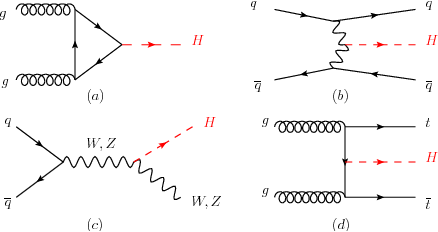
\includegraphics[width=0.95\textwidth]{plots_and_figures/chapter2/higgs_prod.png}
   \caption{ Feynman diagrams for Higgs production modes at LHC: (a) gluon-gluon fusion, (b) vector boson fusion, (c) associated production and (d) ttH~\cite{higg_prod}, are shown.}
   \label{fig:higs_feyn}
 \end{center}
\end{figure}


\begin{figure}[hbtp]
  \begin{center}
    \captionsetup{width=.8\textwidth}
   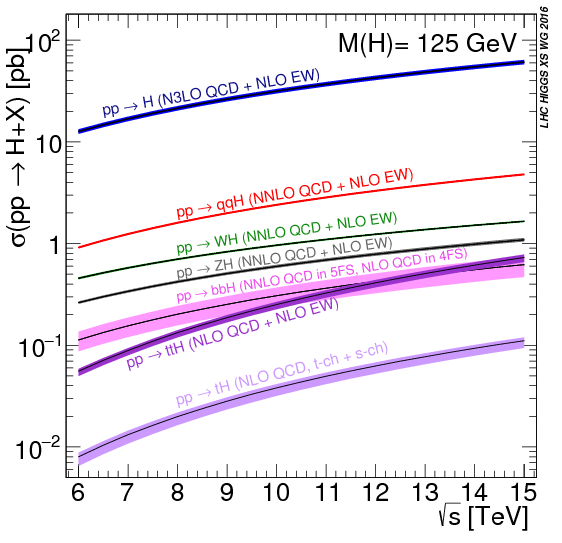
\includegraphics[width=0.9\textwidth]{plots_and_figures/chapter2/higgs_xs.png}
   \caption{The SM Higgs boson production cross-section as a function of the center-of-mass energy in proton-proton collisions at the LHC~\cite{higg_prod}.}
   \label{fig:higs_xs_som}
 \end{center}
\end{figure}
    
\begin{figure}[hbtp]
  \begin{center}
    \captionsetup{width=.8\textwidth}
   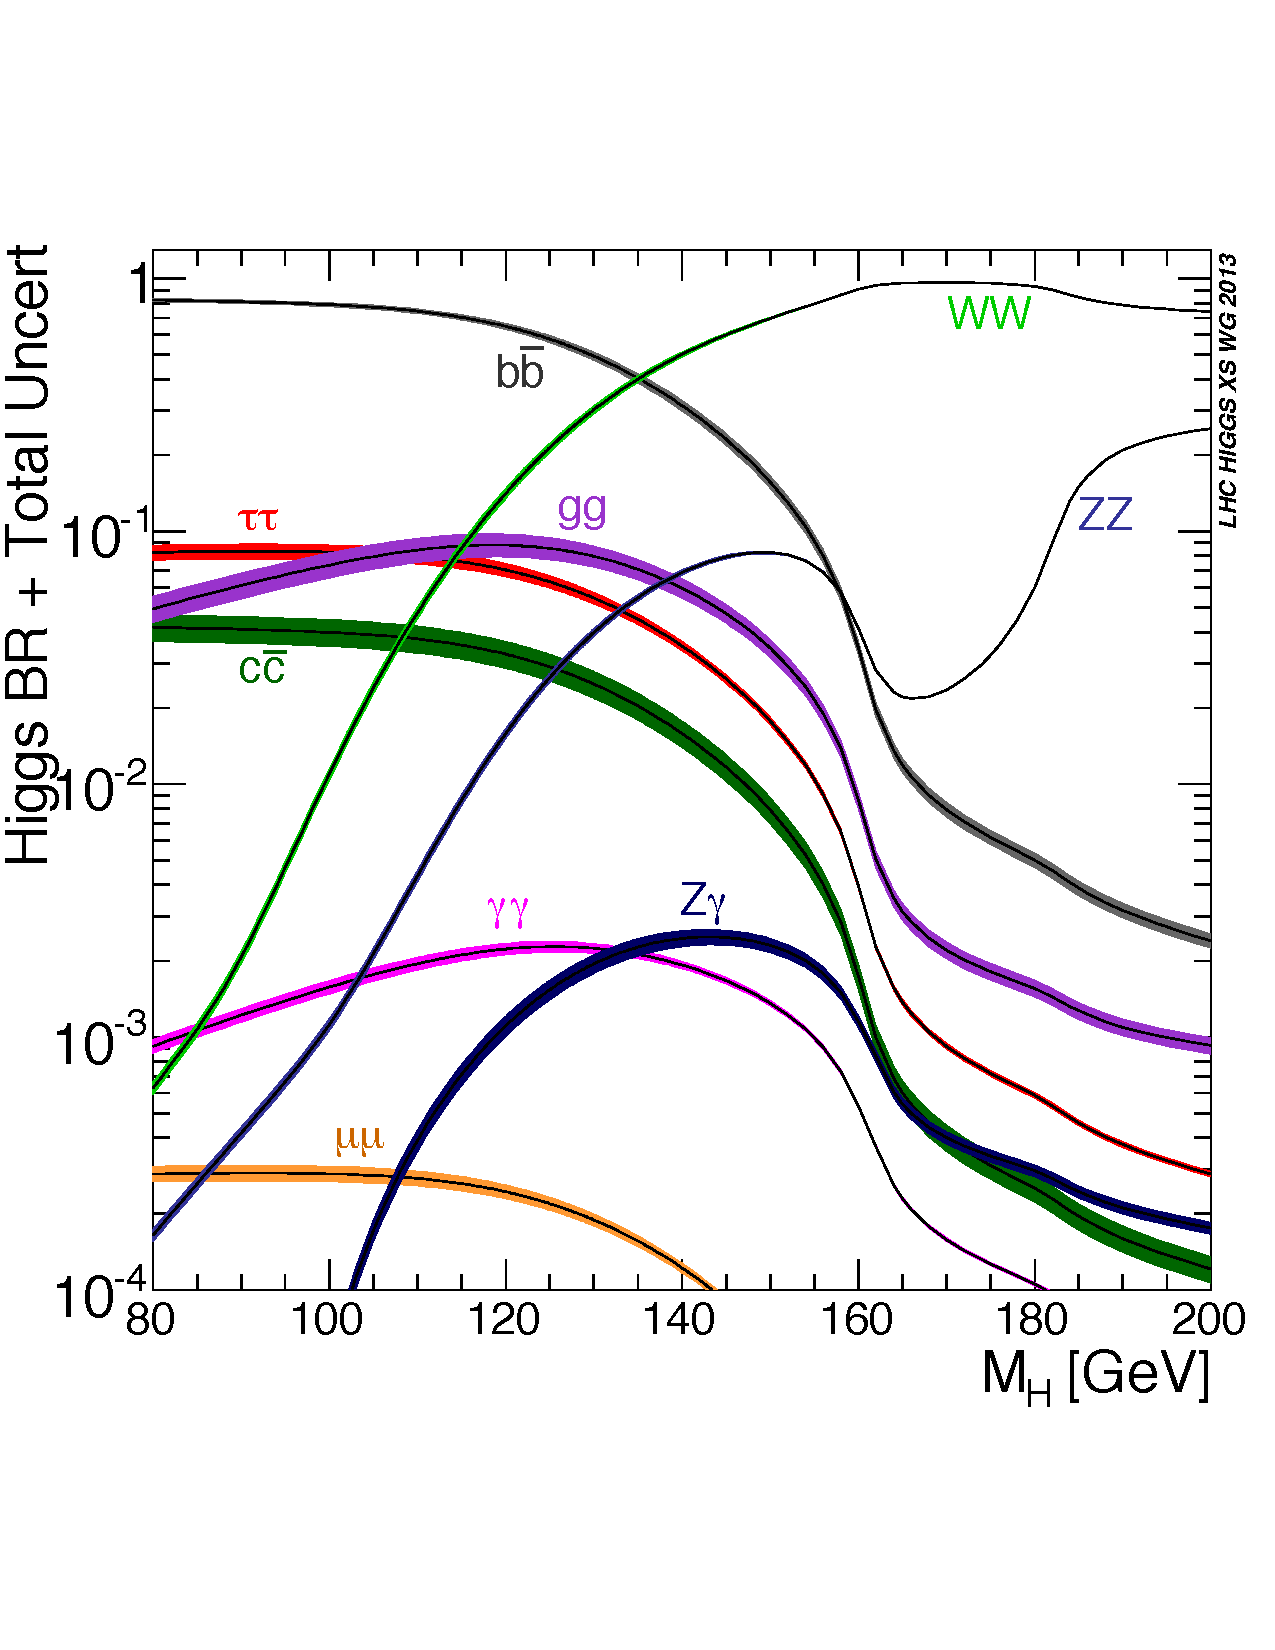
\includegraphics[width=0.9\textwidth]{plots_and_figures/chapter2/higgs_decays.pdf}
   \caption{Branching fractions to SM decays of the Higgs boson as function of mass~\cite{hg_decay}.}
   \label{fig:higs_decays}
 \end{center}
\end{figure}

\section{Inadequacies of the SM}
Despite being a faithful description of nature, the SM is not perfect. There are several motivations that suggest the existence of physics beyond the SM. We outline some of these here.

To start, the SM falls short of being an ideal theory of everything, because it doesn't include gravitation. Including gravitational interaction into the SM has proven to be a difficult challenge. It hasn't yet been possible to incorporate the most successful theory of gravity, General Relativity, and the SM into a single framework. Secondly, neutrinos which are electrically neutral leptons (see section ~\ref{fermions}) are strictly massless within the SM. However, it has been well-established by experiments that neutrinos oscillate (change flavor). This is only possible if neutrinos have mass. The small but finite masses that neutrinos are now known to have doesn't fit with the SM formulation. Thirdly, cosmological observations point to the existence of a type of matter and energy, the origin of which cannot be explained within the SM. They are referred to as dark matter and dark energy. About 26\% of the universe is known to be made of dark matter and 69\% is known to be made of dark energy. Thus, particles of the SM form only 5\% of the observable universe. Finally, it is believed that matter and anti-matter were produced in almost equal amounts at the Big Bang. However, the universe is made almost entirely of matter. There is no mechanism in the SM that explains how we ended up with a matter dominated universe. Besides the unexplained phenomena outlined above, our understanding of some theoretical features of the SM is inadequate. The SM contains no less than 19 numerical free parameters. The values of these parameters are known but we do not have an understanding of their origins.

To address such shortcomings, many theories have been proposed that modify the SM in such a way that they are consistent with existing observations, but at the same time try to address its imperfections. These theories, called BSM (beyond the standard model) theories predict many outcomes that are otherwise not allowed by the SM. The recently discovered h unlocks a portal to look for these outcomes. As mentioned earlier, the constraint on the branching fraction to non-SM decay modes of the h, derived from a combined study by CMS and ATLAS is B(non-SM) $<$ 34\% at 95\% confidence level (CL)~\cite{JHEP2016:45}. These limits suggest a significant contribution from exotic (non-SM) decays in the BSM Higgs sector. One such interesting process that is forbidden in the SM but occurs in many new physics scenarios is interactions between charged leptons that violate the conservation of Lepton Flavor. In particular, Lepton Flavor Violating (LFV) decays of the h are allowed by these theories, and could be realized in decays of the h, which is neutral, into two charged leptons of different flavor. Looking for LFV decays of charged leptons is also interesting in the light of neutrino oscillations mentioned earlier, which also violate lepton flavor, a phenomenon that remains unexplained by the SM~\cite{th_kell}.


\section{BSM models with lepton flavor violation}
\label{sec:BSM}
Like all fermions, charged leptons acquire mass from their interaction with the Higgs. Higgs interacts with these leptons via Yukawa couplings. The Yukawa interaction matrix is diagonal in SM:

\[
  Y=\begin{pmatrix}
    Y_{ee}       & 0 & 0  \\
    0       & Y_{\mu\mu} & 0  \\
    0       & 0 & Y_{\Pgt\Pgt}
  \end{pmatrix}
\]

However, in BSM models, the above doesn't hold true~\cite{Harnik:2012pb} and off-diagonal Yukawa couplings are possible. In a model containing only the SM Higgs as the source of EWSB, an effective field theory approach can be used to introduce off-diagonal couplings~\cite{DiazCruz:1999xe}. If only SM particles (quarks, leptons, gauge and Higgs bosons) are considered to exist up to a certain energy scale, $\Lambda$, additional heavy fields can be integrated out, leading to an effective field theory. Higher dimensional operators of dimension 6 then suffice to introduce LFV couplings. Interestingly, dimension 5 operators introduce neutrino oscillations into the SM, but not LFV in interactions of charged leptons. Dimension 6 operators decouple the values of fermion couplings to the h from the fermion masses. The Yukawa couplings can be then written as:
\begin{equation}
  Y_{ij}=\frac{m_{ij}}{v}\delta_{ij}+\frac{v^2}{\sqrt{2}\Lambda^2}\hat{\lambda}_{ij}
\end{equation}
where $\hat{\lambda}_{ij}$s are coefficients associated with dimension 6 operators. In the limit $\Lambda\rightarrow\infty$, we recover the SM and off-diagonal couplings are zero. Thus, LFV couplings can be introduced as long as the mass scale is finite.  In BSM models with several sources of EWSB, LFV couplings can be introduced without this restriction. Two Higgs doublet models (2HDM) models constitute general models of this class, and allow the violation of lepton flavor~\cite{PhysRevLett.38.622}. Supersymmetry models~\cite{Han:2000jz,Arganda:2004bz,Arhrib:2012ax,Arana-Catania:2013xma,Arganda:2015uca,Arganda:2015naa}, such as the Minimal Supersymmetric Standard model (MSSM) and the Next-to-Minimal Supersymmetric Standard model (NMSSM), also postulate multiple Higgs bosons, and give rise to LFV interactions. Supersymmetric models introduce a alternate (supersymmetric) boson partner to every SM fermion and an alternate fermion partner for every SM boson. These alternate particles, if discovered, could be suitable candidates for explaining dark matter and dark energy. Other models that allow LFV interactions include~\cite{HIG-17-001} composite Higgs models~\cite{Agashe:2009di,Azatov:2009na} which consider the SM h to be a bound state of other BSM particles, partially composite Higgs models such as Randall-Sundrum models~\cite{Perez:2008ee,Casagrande:2008hr,Buras:2009ka}, and several others~\cite{Blanke:2008zb,Giudice:2008uua,AguilarSaavedra:2009mx,Albrecht:2009xr,Goudelis:2011un,McKeen:2012av,Pilaftsis199268,PhysRevD.47.1080,Arganda:2014dta,Ishimori:2010au}.

\section{Pre-LHC constraints on LFV couplings}

Indirect low-energy measurements from pre-LHC era can be used to constrain the $\hmu$ decay. These constraints were derived and summarized in~\cite{Harnik:2012pb}. For example, constraints on $\Pgt\rightarrow\Pgm\gamma$ transition which proceed via a virtual Higgs boson can be used to constrain $\hmu$ decay. Feynman diagrams contributing to this process at one loop level are shown in Figure~\ref{fig:prelhclfv}. Further constraints come from $\Pgt\rightarrow 3\Pgm$ decays, and also from anomalous magnetic dipole moments, and are shown in the same figure. The constraints on Yukawa couplings derived from the above measurements can be converted to constraints on $Br(\hmu)$, following the procedure described in Section~\ref{results}. These constraints set the upper limit on $Br(\hmu)\lesssim 10\%$, thus leaving a lot of room to search for this decay. Similar constraints exist for $\he$ LFV decay, and are set at $Br(\he)\lesssim 10\%$. Indeed, CMS searches looking for $\he$ decay have been performed along with searches for $\hmu$. Finally, it is interesting to note the LFV decay, $\hflep$, is very strongly constrained by $\Pgm\rightarrow\Pe\gamma$ decays, giving an very stringent upper limit $Br(\hflep)\lesssim 2\times10^{-8}$. Due to such strong existing constraints, this search is not been performed by CMS, but rather $\hmu$ (this thesis) and $\he$ searches are performed.           

\begin{figure}[hbtp]
 \begin{center}
   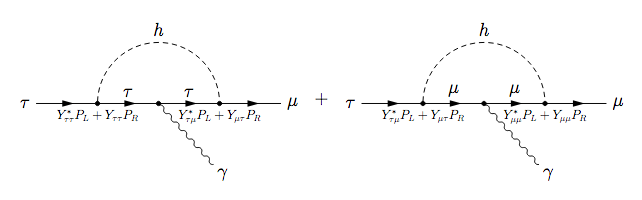
\includegraphics[width=0.9\textwidth]{plots_and_figures/chapter2/tau_mugamma.png}\\
   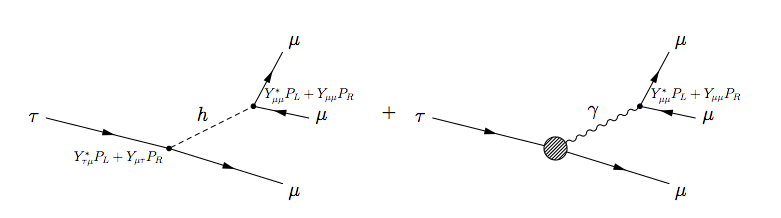
\includegraphics[width=0.9\textwidth]{plots_and_figures/chapter2/tau_3mu.png}\\
   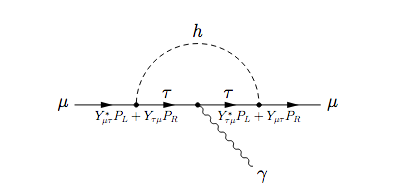
\includegraphics[width=0.6\textwidth]{plots_and_figures/chapter2/dipole.png}
   \caption{Diagrams contributing to flavor violating process $\Pgt\rightarrow\Pgm\gamma$ (top), $\Pgt\rightarrow 3\Pgm$ (middle) and anomalous magnetic moment of the muon (bottom)~\cite{Harnik:2012pb}.}
   \label{fig:prelhclfv}
 \end{center}
\end{figure}

\section{Constraints from previous LHC searches}

The first direct search for LFV Higgs decays was published by CMS collaboration in 2015~\cite{Khachatryan:2015kon}. This search improved the limits listed above by an order of magnitude to $\mathcal{B}(\hmu)<1.51\%$ (0.75\%) for observed (expected) limits at 95\% CL. This was followed by another search (2016) which set observed (expected) upper limits on the branching fractions  $\mathcal{B}(\he)<0.69\%$ (0.75\%) at 95\% CL~\cite{HIG-14-040}. Both searches were performed with 19.7\,$\mathrm{fb}^{-1}$ of pp collision data collected at 8 TeV center-of-mass energy by CMS during Run I of LHC . The limits from these searches are summarized graphically in Figure~\ref{fig:8tev_limits}. In 2015 and 2017, the ATLAS Collaboration also published results from similar searches performed with data collected by the atlas detector~\cite{Aad:2016blu,Aad:2015gha}. The observed (expected) limits were set at $\mathcal{B}(\hmu)<1.43\%$ (1.01\%) and $\mathcal{B}(\he)<1.04\%$ (1.21\%) at 95\% CL.

\begin{figure*}[hbtp]
  \begin{center}
   \captionsetup{width=.7\textwidth,justification=centering}
   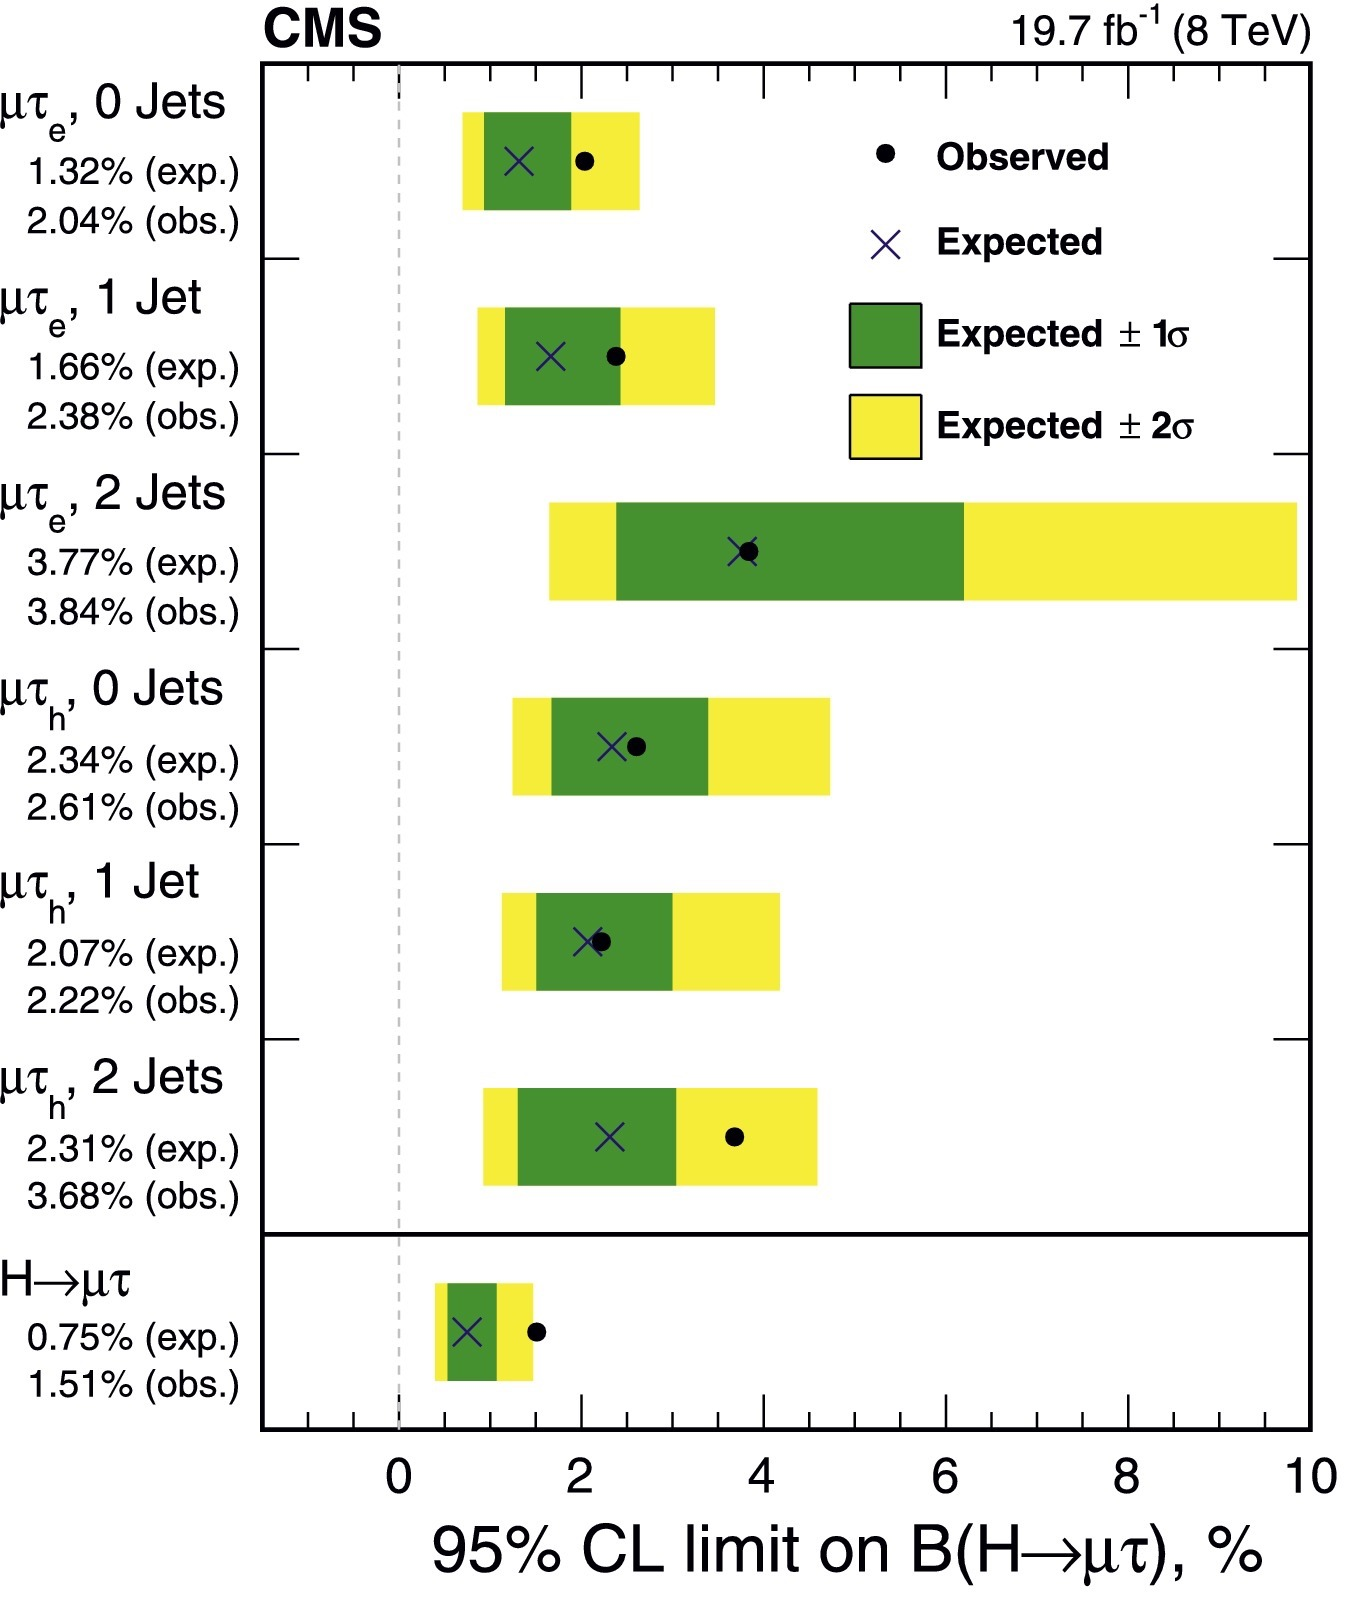
\includegraphics[width=0.6\textwidth]{plots_and_figures/chapter2/mutau_limits.jpg}\\
   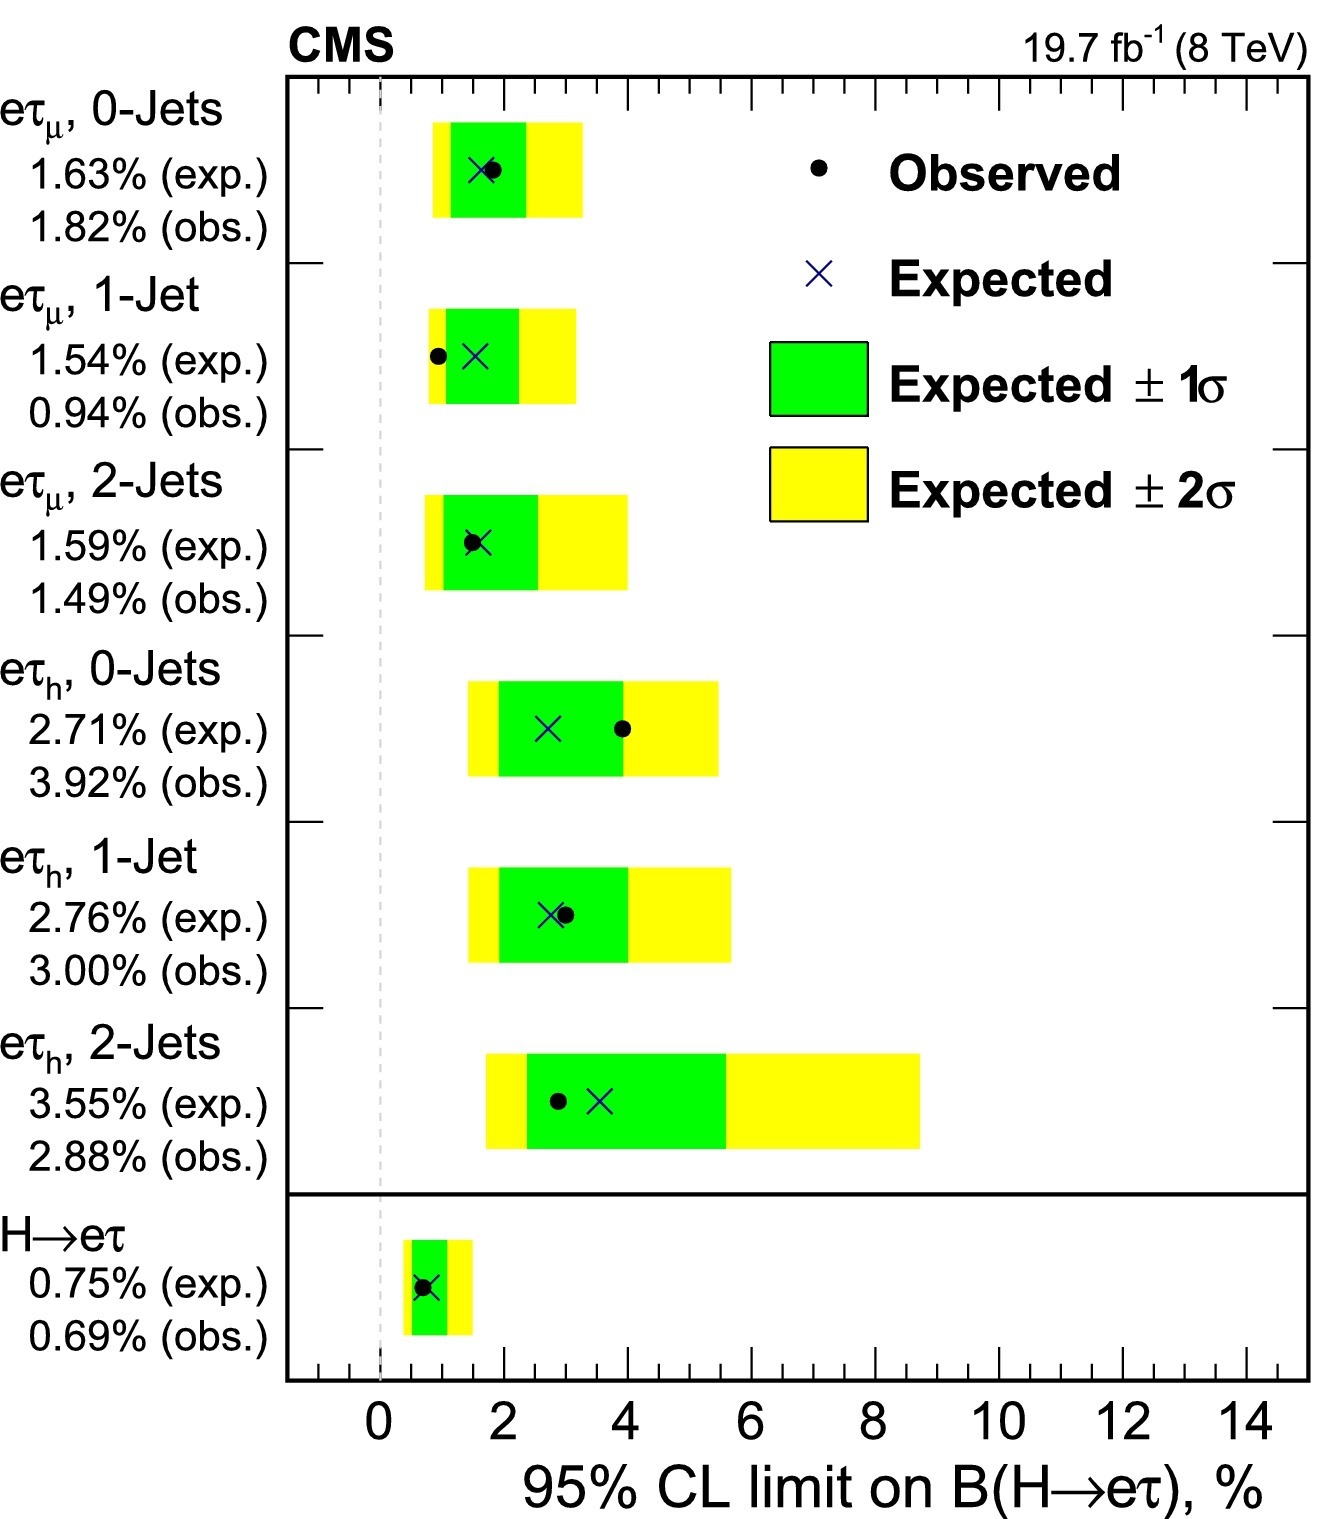
\includegraphics[width=0.6\textwidth]{plots_and_figures/chapter2/etau_limits.jpg}
   \caption{Limits from Run I searches performed by CMS for $\hmu$ (top) and $\he$ (bottom)~\cite{Khachatryan:2015kon,HIG-14-040}.}
   \label{fig:8tev_limits}
 \end{center}
\end{figure*}


The 2015 CMS search for $\hmu$ saw an excess of events with a significance of 2.4\,$\sigma$. Although this excess is not quite enough to claim evidence for this decay, this gives us a strong motivation to perform this search with a larger amount of data which would either lead us to confirm this excess, or squash it and set much stricter limits on this process. The dataset collected by the CMS detector in 2016 provides us with such an opportunity. It corresponds to proton-proton collision data at a much higher center-of-mass energy of 13\,TeV. The number of h bosons produced depends on the cross-section. Since the cross section scales up at higher center-of-mass energies (see Figure~\ref{fig:higs_xs_som}), a much larger number of h bosons would be produced. Also, the 2016 dataset has a size of 36\,$\mathrm{fb}^{-1}$ which is almost two times in size of the run I dataset. This thesis describes this search specifically in the channel where the $\Pgt$ decays into a electron, i.e. the $\hmue$ channel.   

\section{Motivations for $\Hmue$ search}
As mentioned in section~\ref{sec:BSM}, many of the BSM models, that allow LFV decays of the h, predict the existence additional heavy Higgs bosons. For example, 2HDM predicts the existence of two heavy neutral Higgs bosons, H(CP-even) and A(CP-odd). According to a theoretical study published in 2016~\cite{PhysRevD.93.055021}, these heavy bosons (henceforth referred to as H) are expected to decay in a Lepton Flavor Violating manner just like their SM counterpart, h . A direct search for $\Hmu$ would thus provide a complementary probe of these BSM models that postulate the existence of such heavy neutral H bosons. In fact, the 2015 CMS search for $\hmu$ was reinterpreted as a search for $\Hmu$ decay~\cite{Buschmann:2016pb}, and limits on $\sigma(\textrm{gg}\rightarrow \PH)\times\mathcal{B}(\Hmu)$ were set for H bosons in the mass range of 150\,GeV to 300\,GeV. We describe here the first direct search to look for $\Hmu$ decay, in the channel where the $\Pgt$ decays into an electron, i.e. $\Hmue$ channel. Only the primary H production mode (gluon fusion) is considered for this search. This search uses the same dataset as the $\hmu$ search, i.e. 36\,$\mathrm{fb}^{-1}$ of pp collision data at 13 TeV center-of-mass energy collected in 2016, and probes H masses in the range range $200<m_H<900$\,GeV. 



%
% Chapter 3
%

%%
% Modified by Megan Patnott
% Last Change: Jan 18, 2013
%
%%%%%%%%%%%%%%%%%%%%%%%%%%%%%%%%%%%%%%%%%%%%%%%%%%%%%%%%%%%%%%%%%%%%%%%%
%
% Modified by Sameer Vijay
% Last Change: Wed Jul 27 2005 13:00 CEST
%
%%%%%%%%%%%%%%%%%%%%%%%%%%%%%%%%%%%%%%%%%%%%%%%%%%%%%%%%%%%%%%%%%%%%%%%%
%
% Sample Notre Dame Thesis/Dissertation
% Using Donald Peterson's ndthesis classfile
%
% Written by Jeff Squyres and Don Peterson
%
% Provided by the Information Technology Committee of
%   the Graduate Student Union
%   http://www.gsu.nd.edu/
%
% Nothing in this document is serious except the format.  :-)
%
% If you have any suggestions, comments, questions, please send e-mail
% to: ndthesis@gsu.nd.edu
%
%%%%%%%%%%%%%%%%%%%%%%%%%%%%%%%%%%%%%%%%%%%%%%%%%%%%%%%%%%%%%%%%%%%%%%%%

%
% Chapter 2
%

\chapter{Experimental Setup}
\label{chap:exper_setup}
..intoduce...
\section{The Large Hadron Collider}
\label{sec:LHC}

The Large Hadron Collider (LHC) is a powerful proton-proton synchrotron. It was built and is operated at the European Center for Nuclear Research (CERN) and is situated about 100 m underground close to Geneva, Switzerland. It has a circumference of 26.7 km and uses a tunnel previously built for LEP (Large Electron Positron Collider). Being a particle-particle collider, it consists of two rings with counterrotating beams which are steered using magnets and accelerated using radiofrequency resonating cavities. These beams are made to intersect at four collision points around the LHC ring, at one of which rests the CMS detector. Besides proton-proton collisions the LHC can also collide heavy ions (lead-lead collisions) or heavy ions with protons (lead-proton collisions). Since starting operation in September 2008 the LHC has been the world's most powerful apparatus and will probably remain so in the forseeable future. The following section describes proton-proton collisions at the LHC as the data used in the subsequent physics analysis corresponds to events from these collisions.

The injector chain that supplies protons to the LHC consists of four CERN accelerators that actually predate the LHC: Linac 2, PSB (Proton Synchroton Booster), PS (Proton Synchotron) and SPS (Super Proton Synchotron). This is illustrated in figure~\ref{fig:cern_acc_comp}. The proton source is simply tank of hydrogen gas. The hydrogen atoms are ionized to yield protons which are then fed in the Linac 2, a linear accelerator. This accelerates the protons to an energy of about 50 MeV which are then fed into a series of circular accelerators starting with the PSB which accelerates the protons to 1.4 GeV. The PS then accelerates them to 25 GeV and they are then sent to the SPS which accelerates them to 450 GeV before being finally fed into the LHC beampipe. Inside the LHC the protons are accelerated by sixteen radiofrequency cavities which are made to oscillate at 400 MHz and the proton beam is sorted into discrete packet called 'bunches'. The beam is steered by 1232 Niobium-Titanium superconducting dipole magnets and collimated using quadrupole magnets. This magnet system is kept at a temperature below 2 K, using a pressurised bath of superfluid helium at about 0.13 MPa, and operates at fields above 8T. The LHC has three sophisticated vacuum systems: the insulation vacuum for cryomagnets, the insulation vacuum for  helium  distribution, and the beam vacuum.

\begin{figure*}
\begin{center}
\includegraphics[width=0.8\textwidth,keepaspectratio]{plots_and_figures/cern_acc_complex.png}
\caption{Cern Accelerator Complex}
\label{fig:cern_acc_comp}
\end{center}
\end{figure*}


It takes about 4 minutes and 20 seconds to fill up the each of the LHC rings wih protons, and about 20 minutes for the proton beam to reach its current peak energy 6.5 TeV. At this point, each LHC beam contains 2808 bunches each consisting of $1.5 \times 10^{11}$ protons, and colliding at a center of mass energy of 13 TeV. It is anticipated for the COM energy to increase to 14 TeV in 2018. Looking for physics beyond the standard model by colliding protons at such high energies is one of the primary aims of the LHC.

Another important parameter for a collider like the LHC is the instantaneous luminosity, \mathscr{L}.




So why do gnus do what they do?  This is a perennial question that has
yet to be answered definitively by scientists.  Is their future
somehow tied inexplicably with that of humans?  Hard to say, but we do
feed them a lot.  It has even been theorized that rotundness is a
symbol of status or class within the Gnus; those who are more
productive (i.e., cute, furry, friendly) will be fed more than those
who are less so.  So the more rotund, the higher status one has in the
Gnu society.

One could extrapolate this to mean that there is a super-Gnu out there
somewhere; the biggest, rotundest Gnu that you've ever seen, probably
of epic proportions!  This would have to be the Leader of Gnus, or LoG
for short.  But the LoG would definitely have to be the cutest,
furriest, and most friendly Gnu that you've ever seen.

\subsection{The LoG}

So how does the LoG get chosen?  Ultimately by humans.  So we can say
that the Gnu society is perhaps the truest democracy that has ever
existed; the leader is chosen by merit, and chosen by complete
outsiders.  As such, the LoG must truly epitomize all that Gnus stand
for: opposedness to overmanagement, cuteness, friendliness, and
furriness~\citep{gloonson98:_gnuly_discov_gnus}.  The gnus themselves
vote at an anual election, based upon these attributes (campagaining
is an anethema to Gnus; see Section~\ref{sec:groovin-gnus}).

\section{Physics beyond the standard model}
\label{sec:BSM}

Table~\ref{tbl:votes} shows the latest electoral college voting by the
LoG for the year 2000.  Each Gnu is scored on a scale of one to ten on
the attributes described above.  The results shown in the table are
average scores in each category for all votes; the Gnu's final score
is shown in the final column.

%
% Be aware that page-spanning tables a Very Odd Creatures.  The
% "longtable" environment in LaTeX does some deep Voodoo to make
% everything work out properly.  One of its deep incantations is to
% make the table appear as though it is double spaced.  You can fix
% this by trailing each line with "\\[-6em]" instead of just "\\".
% When using longtable it is also important to compile your file
% more than once. But you're probably already doing this to get
% the internal references correct, anyway.
%

\begin{center}
  \begin{longtable}{lccccc}
    \caption{Electoral College Results for the \NoCaseChange{LoG} Election in the Year
2000\label{tbl:votes}\/}\\
        \toprule
        Candidate\footnote{note all names begin with G} & Anti-management & Cuteness & Friendliness & Furriness & Aggregate \\
        \midrule
\endfirsthead % Everything above goes at the top of the 1st page only
% As with the first header, we don't want obscene amounts of space for
% subsequent headings either, and eliminate an em of whitespace.
  \caption[]{{\em Continued}}\\
  \midrule
  Candidate & Anti-management & Cuteness & Friendliness & Furriness & Aggregate \\
  \midrule
\endhead % Everything above here (and below the \endfirsthead) goes at the top
         % of continuation pages.  The [] argument prevents a duplicate
         % entry from appearing in the table of contents.
% The following 3 lines are provided as an example only -- per ND
% guidelines, the footer at the bottom of a page for a longtable
% should not have a bottom line.  Only the absolute bottom of the
% table should have a final \bottomline

%  \midline
%  \multicolumn{6}{|r|}{\textit{continued}\ldots} \\
%  \bottomrule
\endfoot % The above section goes at the bottom of continuation pages
  \bottomrule
\endlastfoot % The very last bottom of the table
    Glen & 6.2 & 7.0 & 6.1 & 9.8 & 7.2 \\
    Goober & 6.9 & 2.1 & 5.7 & 4.1 & 4.6 \\
    Genevra & 2.2 & 2.0 & 1.1 & 1.1 & 1.6 \\
    Greg & 8.3 & 0.4 & 1.1 & 9.5 & 4.8 \\
    Gina & 6.0 & 7.8 & 6.4 & 4.9 & 6.2 \\
    Geof & 1.1 & 8.7 & 3.7 & 7.3 & 5.2 \\
    Grendel & 2.8 & 1.7 & 3.4 & 3.2 & 2.7 \\
    Geronimo & 1.2 & 1.2 & 8.8 & 2.2 & 3.3 \\
    Gabrielle & 4.7 & 3.6 & 0.8 & 2.0 & 2.7 \\
    Giovani & 8.4 & 5.8 & 3.4 & 7.4 & 6.2 \\
    Graham & 4.7 & 5.8 & 5.3 & 0 & 3.9 \\
    Gil & 5.9 & 4.0 & 5.5 & 7.6 & 5.7 \\
    Gerald & 2.0 & 3.7 & 8.0 & 4.3 & 4.5 \\
    Guilani & 7.7 & 3.9 & 2.7 & 6.4 & 5.1 \\
    Guido & 7.6 & 4.3 & 6.5 & 1.0 & 4.8 \\
    Godzilla & 5.1 & 2.2 & 5.3 & 6.9 & 4.8 \\
    Gail & 5.7 & 7.9 & 4.1 & 1.0 & 4.6 \\
    Garth & 4.7 & 7.1 & 2.5 & 3.0 & 4.3 \\
    Gavin & 1.1 & 9.5 & 0.4 & 8.0 & 4.7 \\
    George & 9.5 & 4.5 & 9.1 & 7.5 & 7.6 \\
    Gunnar & 1.4 & 5.8 & 4.8 & 6.2 & 4.5 \\
    Gillian & 7.6 & 9.0 & 6.4 & 4.6 & 6.9 \\
    Greta & 1.5 & 0.5 & 0.9 & 7.7 & 2.6 \\
    Gabby & 1.2 & 3.3 & 7.0 & 2.1 & 3.4 \\
    Gaetena & 6.8 & 1.9 & 4.1 & 8.3 & 5.2 \\
    Ganet & 2.3 & 1.1 & 8.5 & 7.3 & 4.8 \\
    Gardenia & 1.8 & 9.5 & 9.9 & 3.0 & 6.0 \\
    Genna & 5.2 & 3.7 & 3.4 & 3.8 & 4.0 \\
    Genesis & 1.7 & 8.3 & 6.7 & 4.9 & 5.4 \\
    Genaveve & 4.7 & 8.9 & 3.4 & 9.2 & 6.5 \\
    Gene & 3.3 & 6.9 & 0.6 & 5.5 & 4.0 \\
    Gilda & 5.2 & 4.6 & 9.9 & 1.4 & 5.2 \\
    Goldie & 8.9 & 9.1 & 2.0 & 8.2 & 7.0 \\
    Grace & 5.9 & 3.2 & 3.1 & 4.3 & 4.1 \\
    Gretchen & 4.5 & 6.5 & 1.6 & 1.3 & 3.4 \\
    Garrick & 4.8 & 5.7 & 9.4 & 5.1 & 6.2 \\
    Gallagher & 7.4 & 0.4 & 7.6 & 0.4 & 3.9 \\
    Gerry & 1.4 & 8.8 & 4.7 & 0.5 & 3.8 \\
    Gertrude & 9.1 & 8.3 & 0.4 & 5.5 & 5.8 \\
    Gehosephet & 6.6 & 2.9 & 8.3 & 4.4 & 5.5 \\
    Gohn & 8.7 & 2.6 & 7.4 & 2.3 & 5.2 \\
    Gibby & 8.7 & 6.9 & 4.7 & 7.2 & 6.9 \\
  \end{longtable}
\end{center}

As you can see from Table~\ref{tbl:votes}, George (my favorite Gnu)
won for the year 2000, with an aggregate score of 7.6.

% % uncomment the following lines,
% if using chapter-wise bibliography
%
% \bibliographystyle{ndnatbib}
% \bibliography{example}



%
%
% Chapter 4
%

\chapter{Object reconstruction and event generation}
\label{chap:event_sim}
\section{Introduction}
\label{intro}
This chapter is divided into two parts. In the first part, the procedure for the generation of simulated events is described. This is done in several distinct stages with the output of one stage serving as an input for the next. A suite of software packages, developed mostly by the particle and nuclear physics communities, is used to achieve this. This part concludes by detailing the simulated datasets used in the analyses described in this thesis. In the second part of this chapter, the reconstruction of physics objects is described in detail. It starts with a description of the particle-flow algorithm which is kind of a global event reconstruction scheme for the entire event. This is followed by descriptions of track , muon and electron reconstructions. Reconstruction of jets is described next followed by description of composite objects used in the analysis such as collinear mass and transverse mass. Brief desciptions of tau lepton reconstruction and b-tagging of jets is also included.


\section{Event Simulation}
A $pp$ collision at the LHC, like any hadronic collision, is more complex than the hard interaction of two participating partons. The proton being a composite object, the colliding partons from the hard interaction are accompanied by other quarks and gluons that interact and rearrange themseleves into colorless objects. A $pp$ collision thus consists of: the Hard Scattering which represents the part of the collision where two partons in the initial state interact by exchanging a high transverse momentum, and the Underlying Event that represent the interaction of the everything else in the collision except the partons in hard scattering. In addition to the implementing the above, i.e. physics of a $pp$ collision  that produces a bunch of final state particles, the event simulation also has to include interactions of these particles with the CMS detector. Monte Carlo methods, that use generation of random numbers to simulate sampling from a given probability distribution , are used to model the above event simulations~\cite{mc_evtsim}.

\subsection{Monte Carlo method}

Monte Carlo (MC) methods (named after a famous casino in the city state of Monaco) are a broad class of computational algorithms that rely on repeated random sampling to obtain numerical results~\cite{mcwiki}. In particle physics, these methods play a key role in generation of events and are used primary for : generation of samples from specified probabilty distributions, and the calculation of integrals. Programs which implement the above method, called MC event generators, use generation of random numbers to make decisions about physics processes. These can range from selection of processes are generated in the collision, to which decay channel a particle decays in, to making decisions on how the particle interacts with detector material. Usually, each such decision is the result of a draw from a distribution which depends only on the current state the process is in, and not on previous states. The MC generator is provided as input the distributions that represent the physics of the generated particles, their production, their decay modes and their couplings. A MC generator starts by using a pseudo-random number generator that usually outputs a random number between 0 and 1 with. Although, true random number generation can only be done by physical processess, modern pseudo-random number generators are known to generate numbers with a high degree of randommness. Starting from this distribution, the MC event generator uses one of the various methods such as the inverse-transform method, or the rejection sampling method to convert this uniform distribution into a desired probablity distribution, $p(x)$. It is then possible to generate random numbers according to this distribution to simulate physical processes. 


\subsection{CMS simulation pipeline}

The MC simulation of events in CMS consists of the following sequential steps. The first step is simulation of the Hard Scattering.As mentioned earlier, this represents the primary hard interaction in a collision where two partons in the initial state interact by exchanging high transverse momentum resulting in a final state with two or more partons. The parton density function (pdf) which parametrizes the distributions of the partons inside each hadron are used to model the momenta of incoming partons. It represents the probability of finding a parton of a certain flavour at a certain longitudinal momentum fraction, when the hadron, that contains it, is probed at a certain scale. The PDF are extracted from fits to the data, mainly from ep collisions, and various PDF sets are available for each parton flavour. Commonly used pdf sets include ones provided by the  CTEQ, HERA (H1 and ZEUS) and NNPDF collaborations. The LHAPDF library provides a unified C++ interface to all major PDF sets. The matrix element formulation is used to model the hard scattering process to leading order in perturbative QCD, or to higher orders depending on the generator. The next step is simulation of the parton shower. The hadronization and radiation of quarks and gluons in the initial and final states cannot be feasibly encapsulated in the matrix element computation. Parton shower describes these missing parts. The matrix element calculations are combined with the parton shower by one of the different matching schemes which ensure that there is no double counting of terms present in both the matrix element and the partion shower expansion. The matching schemes that are most often used are MLM~\cite{mlm}, CKKW~\cite{ckkw} and FxFx~\cite{Frederix:2012ps}. The simulation of the Underlying Event comes next. Underlying event includes everything in the collision that is not associated with the primary hard scattering process. They consist mostly of soft QCD interactions, and implemented using the MC event generators and interfaced with the matrix element simulation. The hadronization of the quarks and gluons is simulated next and it conisists of recombination of individual partons into colorless hadrons. Lastly the decay of short-lived particles is simulated.

An important part of the event generation chain is the simulation of pileup. The protons circulate inside the LHC not as a continuous beam but in discrete closely packed bunches. This leads to more than one proton-proton collision per bunch crossing, i.e. pileup both in-time and out-of-time (see chapter~\ref{chap:exper_setup}). Event generators add  pile-up events to the hard scattering samples by randomly simulating soft inelastic collisions and overlapping them. The distribution of the number of pileup interactions in data is hard to predict. MC event generators usually produce events for a scenario with a higher number of pileup vertices, and with a flat disctribution of number of vertices . This is afterwards reweighted to match the observed distribution of pileup interactions in data.

Several MC generators have been developed. Some of these can produce all components of the above simulation pipeline while some calculate only the matrix element and need to be interfaced with other generators for the simulation of remaining parts. Pythia~\cite{Sjostrand:pythia8} and Herwig~\cite{herwig} can produce the entire chain while Powheg~\cite{Nason:2004rx,Frixione:2007vw, Alioli:2010xd, Alioli:2010xa, Alioli:2008tz, Bagnaschi:2011tu}, aMC@NLO~\cite{Alwall:2014} and Madgraph~\cite{Alwall:2011uj} produce up to matrix element stage. Powheg and aMC@NLO can perform next-to-leading order calculations. 

Finally, the Geant4 (GEometry ANd Tracking)~\cite{GEANT4} package is used to simulate the interaction of physical particles after the collision, produced by pipeline described  above, with a sophisticated and complex simulation of the detector itself. This simulated detector response is used as input for the same physics reconstruction algorithms (desribed in the next section), that are used to reconstruct the data, thus enabling a direct comparison of the two. If differences are observed in the behavior of these reconstruction algorithms for MC events in comparsion to observed data, the MC events are tuned to the behavior observed in data. 


\section{MC samples used for the analyses}
\label{samples_mc}

The {ggH} and VBF Higgs boson samples are generated with POWHEG 2.0 while an extension of POWHEG 2.0~\cite{Luisoni:2013kna} is used for the $\PW\PH$ and $\PZ\PH$ simulated samples. For the \Hmue analysis, only the gluon fusion (ggH) production mode has been considered. Samples are generated for a range of H masses from 200 to 900 GeV.

The $\zjets$ and $\wjets$ processes are simulated using the \aMCATNLO generator at leading order (LO) with the MLM jet matching and merging scheme. The same generator is also used for diboson production which is simulated at  next-to-LO (NLO) with the FxFx jet matching and merging scheme. POWHEG 2.0 and 1.0 are used for top quark-antiquark ($\ttb$) and single top quark production, respectively. The POWHEG and MADGRAPH generators are interfaced with PYTHIA 8 for parton showering, fragmentation, and decays. 

As mentioned earlier in this chapter, additional pileup interactions are also a part of the MC generation pipeline. All simulated samples are reweighted to the pileup distribution observed in data. An event weight is applied based on the number of simulated pileup events and the instantaneous luminosity per bunch-crossing, averaged over the run period. Several other scale factors  are used to reweight the events in order to get the MC simulation to match the data closely. These include scale factors based on trigger, lepton identification, lepton isolaton and b-jet tagging efficiencies.

\section{Physics Object Reconstruction}
\label{p_ob_recon}
This section begins with the description of the particle-flow algorithm followed by reconstruction of tracks and vertices, electrons, muons, jets and other physics objects.  
\subsection{Particle Flow}
\label{p_flow}
\subsection{Track and primary vertex reconstruction}
\label{track_recon}

Tracks of charged particles, that traverse the CMS tracker (described in section~\ref{tracker}), are reconstructed~\cite{track_reconstruction} using hits from the pixel and strip detectors in the tracker. Hits are reconstructed by clustering signals above specified thesholds in the pixel and strip channels, and then estimating the cluster positions and uncertainties in a local orthogonal system plane of each sensor. During track reconstruction, a translation is made between the local coordinate system of these hits to the global coordinate system of the tracks. The software used to reconstruct tracks by CMS is called the Combinatorial Track Finder (CTF) and is adaptation of the Kalman filter~\cite{kalman_filter}. Tracks are reconstructed using a iterative procedure with the basic idea being, that tracks that are easiest to find (e.g., high \pt tracks, and produced near the interaction region) are searched in the initial iterations with subsequesnt iterations looking for more difficult sets of tracks (e.g., low \pt tracks , or tracks produced far from the interaction region). Hits unambiguously assigned to the track in the previous iterations are removed for the subsequent ones, thus reducing the combinatorial complexity. Each iteration can be divided into four sequential steps.

The first step is seed generation which provides initial track candidates that define the starting trajectory parameters and associated uncertainties of potential tracks. Charged particles follow a helical paths in the quasi-uniform magnetic field of the tracking requiring a total of five parameters to determine the trajectory. These five parameters are extracted using two or three hits in the inner region of the tracker. The seeds are constructed in the inner part (and then tracks constructed outwards, and not in the opposite manner) because the high granularity of pixel detectors (in contrast to outer strip layers)  ensure low fraction of channels that are hit. Also, particles like pions and electrons interact inelastically with tracker material or lose energy due to bremsstrahlung radiation as they traverse through the tracker to its outer regions making the idea of construcing seeds in the inner region a better choice.

The second step in track generation is track finding which is closely based on the Kalman filter. It extrapolates the seed trajectories along the expected path of a charged particle, beginning with an estimate of the track parameters provided by the trajectory seeds generated in the last step. It then uses the location and uncertainty of detected hits, and estimations of effects such as Coulomb scattering, at successive detector layers, to build track candidates, updating the parameters at each layer. First, using the parameters of the track candidate, evaluated at the current layer, an analytical extrapolation is done that determines which adjacent layers of the detector the trajectory can intersect. This takes into account the current uncertainty in that trajectory just like a Kalman filter. Secondly, a search is perfomed for silicon modules in these layers that are compatible with the extrapolated trajectory. All compatible modules in each layer are then grouped into mutually exclusive groups, such that no two modules in each group overlap. The collection of all hits from from one such module group forms a group of hits. Finally, new track candidates are formed by adding exactly one of the compatible hits from each group, to each original track candidate. The modules in a given group are mutually exclusive and a contribution of more than one hit from each group is not expected. The trajectory parameters of the new candidates are then updated by combining the information from the added hits with the extrapolated trajectory of the original track candidates. Fig~\ref{fig:trackrecon} illustrates the reconstruction efficiency of tracks in case of isolated muons.

The third step in track generation track fitting. In this step the collection of hits from the last step are refitted using a Kalman filter and smoother, to provide a best possible estimate of parameters for each track trajectory. The procedure described above, in conditions as challenging as the LHC, can yields several fake tracks that are not associated with any charged particle passing through the tracker. The fourth and final step applies several quality requirements to set of reconstructed tracks and substantially reduces the fake contribution. The requirements are based on criteria such as the minimum number of layer the track has hits in, how compatible its origin is with a primary vertex, how good a fit they yield etc.

\begin{figure*}
\begin{center}
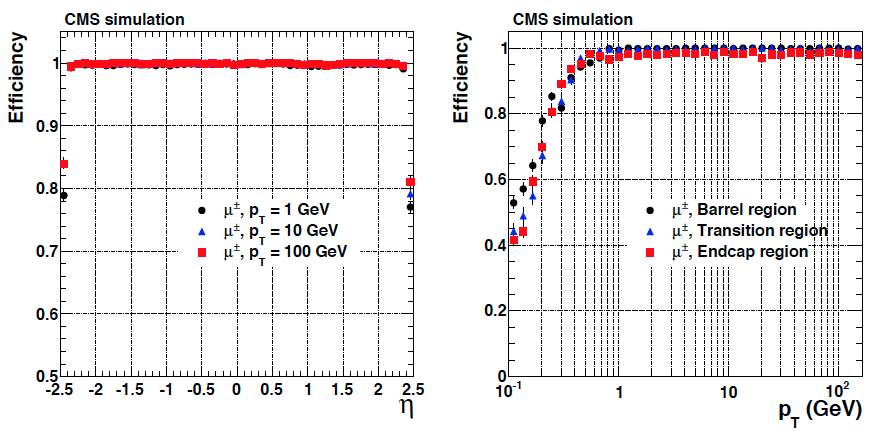
\includegraphics[width=0.9\textwidth,keepaspectratio]{plots_and_figures/chapter4/trackrecon.png}
\caption{Track reconstruction efficencies for single isolated muons as a function of $\eta$ and \pt~\cite{track_reconstruction}.}
\label{fig:trackrecon}
\end{center}
\end{figure*}


Proton-proton interaction vertices are reconstructed by selecting tracks that are produced promptly in the primary interaction region. The selected tracks are then clustered on the basis of their z-coordinatesat their point of closest approach to the centre of the beam spot, which represents a 3-D profile of the region where the LHC beams collide inside the CMS detector. The exact positions of the vertices are then obtained from these clustered candidates, by using a fitting procedure, called the adaptive vertex fitter~\cite{vertex_fitting}. The vertex which has the largest sum of squared transverse momenta of tracks originating from it is considered the primary interaction vertex. 


\subsection{Muon Reconstruction}
\label{mu_recon}
Hits in the muon system (described in section ~\ref{muon_system}) and tracks (muons being charged particles leave tracks in the tracker) from the tracker are used to reconstruct muons~\cite{muon_recon2018}. When muons traverse a muon subdetector (such as RPC, CSC or DT) in the muon system, they ionize the gas in the chambers. The electrical signals produced on the wires and strips as a consequence of the ionization are read out by electronics systems that associate these ``hits'' with well-defined locations in the detector. Various algorithms depending on the subdetector technology are used to reconstruct these hits. Reconstruction of muon tracks using these hits first proceeds independently of track reconstruction in the tracker. These tracks, called \textit{standalone-muon tracks}, are built using these reconstructed hits from the muon system using a Kalman filter. Muon tracks are also built inside-out by propagating tracker tracks (described in previous section) with transverse momentum above 0.5 GeV to the muon system and matching them to (straight-line) segments of hits in DT or CSC. If a match is found, the tracker track qualifies as a \textit{tracker muon track}. Muon tracks are also  built outside-in  by matching standalone-muon tracks with tracker tracks, and combining information from both using a Kalman filter fit. These are called \textit{global muon tracks}. While the global muon reconstruction is especially efficient for muons leaving hits in several muon stations. The \textit{tracker muon} reconstruction is more efficient for low \pt muon candidates but it can also cause fake muon tracks due to hadronic particles which \textit{punch-through} to the innermost muon stations. The \textit{global muon} reconstruction has  high efficiency for muons penetrating through more than one muon station, and reduces the muon misidentification rate compared to tracker muons. Combining both \textit{tracker muon tracks} and \textit{global muon tracks}, the efficiency for reconstructing a muon is as high as 99\%. The particle-flow algorithm applies a set of requirements, based on various quality parameters from muon reconstruction as well as information from other sub-detectors, to  reconstructed candidates. The PF muon candidates used in the analyses described in this thesis were required to satisfy the following set of criterion to be identified as a muon:

\begin{itemize}
\item Must be a global muon or a tracker muon.
\item Must have at least one hit in the pixel subdetector of the tracker
\item $\chi^2$ of the compatibility between the position of the standalone and trackers tracks $<12$
\item Transverse impact parameter of the associated tracker track with respect to the primary vertex $d_{xy}< 2 mm$
\item Longitudinal distance of the (origin of )associated tracker track with respect to the primary vertex $d_z <5 mm$
\item constraints on muon segment matching compatibility between tracker and muon system dependent on if it is a global muon
\end{itemize}
The efficiency of the above selection for muon identification is illustrated using a plot from a study performed by the CMS Muon Physics Object group in Fig.~\ref{fig:muoneff}. As can be seen from the plots, there is a difference in the efficiencies in data and MC simulation. This is corrected using a set a of scaled factors applied as a function $\eta$ and \pt to adjust the efficiency in simulation to get it to match the efficiency in data.  

\begin{figure*}[!htpb]\centering
 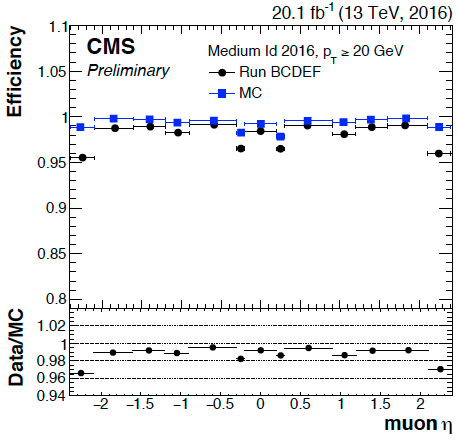
\includegraphics[width=0.47\textwidth]{plots_and_figures/chapter4/muoneffveta.png}
 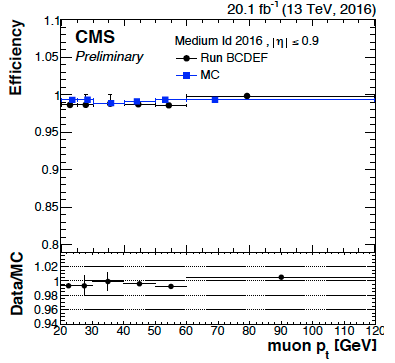
\includegraphics[width=0.49\textwidth]{plots_and_figures/chapter4/muoneffvpt1.png} \\
 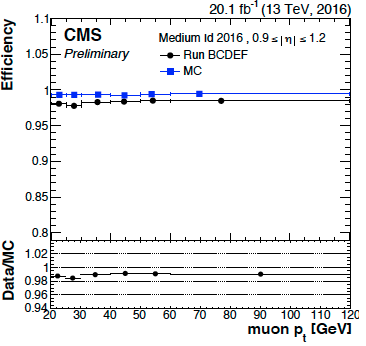
\includegraphics[width=0.49\textwidth]{plots_and_figures/chapter4/muoneffvpt2.png}
 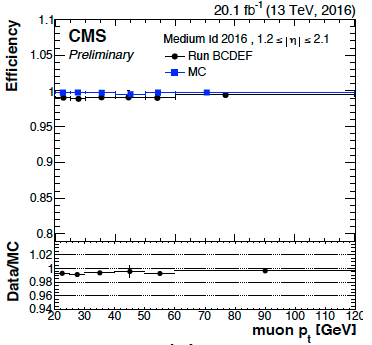
\includegraphics[width=0.49\textwidth]{plots_and_figures/chapter4/muoneffvpt3.png} 
\caption{Efficiency of muon identification as a function of $\eta$ and \pt, for data (black) and simulation (blue)}
 \label{fig:muoneff}
\end{figure*}  
  
The momentum of muons is measured by CMS using one among different possible ways involving the tracker and muon system~\cite{muon_recon2012} and then using the PF algorithm to refine this informmation that exploits information from the full event.



\subsection{Electron Reconstruction}
\label{e_recon}
Besides muons, electron form the other primary part of the final state of the decay we are searching for in this thesis. Electrons, in the CMS, are reconsrtucted using clusters of energy formed in the ECAL (described in section ~\ref{Ecal}) and associating them with tracks from the tracker. The reconstruction of electrons is made complicated by the fact that they can radiate a significant amount of energy before reaching the ECAL. This happens due to the radiation of bremsstrahlung photons caused by the ineraction of electrons with atoms as they pass through the tracker. This loss can range from 33\% to as high as 86\% depending on $\eta$ (as a consequence of the fact that the amount of detector material the electron has to cross is $eta$ dependent). In order to measure the an electron's energy,  clustering algorithms thus need to take into the energy from these bremsstrahlung photon showers together with the deposit made in the ECAL by the electron. The energy from these radiated photons spreads primarily in the $\phi$ owing to bend in electron trajectory in the magnetic field of CMS. The spread in the $\eta$ direction is relatively small. These facts are used by the clustering algorithms.

The algorithm used to cluster the electron energy deposit in the ECAL barrel is called the \textit{hybrid} algorithm. It exploits the above property of the electron shower shape, and uses the geometry of the ECAL to form clusters thare are narrow in $\eta$ direction but wide in $\phi$ direction. Starting with a (seed) crystal containing the largest amount of energy deposited in a considered region above a certain threshold (1 GeV), it adds 5x1 arrays of crystals in $\eta\times\phi$ around the seed crystals in both directions of $\phi$ if the energy contained in the arrays is above another predefined threshold (0.1 GeV). Contiguous arrays are merged into clusters, and finally a electron supercluster is formed from all such strip clusters which have at least one seed strip with energy above another predefined threshold (0.35 GeV). The position of the supercluster is computed as the energy-weighted mean of the cluster positions, whereas its energy is simply taken as the sum of the energy of all its constituent clusters. In the ECAL endcap a different clustering algorithm is used owing to different geometrical arrangement of the crystals. This algorithm called the \textit{5x5} algorithm starts similarly with a seed crystal with maximum energy in a local region, and satisfying the minimum energy requirement of 0.18 GeV. Clusters of 5x5 crystals are progressively grouped around the seed crystal, making a supercluster, if the total cluster energy exceeds 1 GeV and the are withing $\pm 0.7$  and $\pm 0.3$ respectively in $\eta$ and $\phi$ around the seed crystal. The positon and energy of the supercluster is calculates in the same manner as the barrel. The energy from the preshower is also added into the supercluster, using it's most energetic cluster and it's maximum distance in $\phi$ to other clusters and extrapolating it to the preshower plane to define the spread in the preshower. The thresholds used in the above algorithms were optimized using simulation and adjusted durting data taking periods.

The standard track reconstuction (section ~\ref{track_recon}) is not efficient for electrons. This is because the standard approach is compromised by the large radiative losses in the tracker leading to a poor estimation of track parameters. Therefore a dedicated tracking procedure is used for  electron candidated that used infromation not only from the tracker but also the ECAL. Just like the standard track reconstruction procedure the first step in electron track reconstruction is seeding. This is done in two ways and the results are then combined. In the first method, superclusters from ECAL are used. As mentioned earlier, owing to strong magnetic field, the bremsstrahlung photons emitted by the electrons deposit energy in the ECAL at $\eta$ values similar to that of the electron, but at diffrent $\phi$ leading to a spread. The ECAL supercluster algorithms described above recover this energy. The position and  energy of these reconstructed superclusters along with the assumption that the electrons originated close to the center of the beam spot can be used to constrain the trajectory of the electron through the tracker. Hits in the first layers of the trackers compatible with these trajectories are deemed electron seeds. In the second method of seeding, the "opposite" is done. Tracks constructed by the regular tracking algorithm are extrapolated to the ECAL and matched with a supercluster. The seeds corresponding to such matching tracks are retained as electron seeds. The seed collections from these two methods are merged leading to a increase in overall efficiency of the seeding procedure. These seeds are then used to intiate electron track finding phase and fitting phases. This track finding procedure is similar to that used in standard tracking except for small adjustments. The $\chi^2$ fit thresholds used by the Kalman filter to decide whether a hit is compatible with a trajectory (see section~\ref{track_recon} is weakened to accommodate tracks that deviate from their expected trajectory because of bremsstrahlung. Similar adjustments are made to the penalties assigned to track candidates for passing through a tracker layer without being assigned a hit. The final track fit uses a modified version of the Kalman filter, called the Gaussian Sum Filter (GSF), to account for the fact that the energy loss of an electron traversing the tracker material is non-Gaussian. This  makes it unsuitable to use a conventional Kalman filter algorithm which assumes gaussian distribution. The GSF technique deals with this by approximating this non-Gaussian energy-loss distribution as the sum of several Gaussian functions, and is found to perform much better than the regular fitting procedure.

Finally, electron candidates are constructed by associating a electron track (called GSF track) produced by the above procedure with a supercluster in the ECAL. For ECAL-seeded candidates this association is made by a geometrical matching in $\eta-\phi$, while for tracker-seeded candidates a multivariate (MVA) technique that combines information from supercluster and GSF track is used. The electron charge is estimated using a combination of three procedures involving the use the GSF track curvature, use of ECAL supercluster position and its relative postion in $\phi$ to that of the first hit in the GSF track, and also by using KF tracks that have common hits with the GSF tracks. The combination of a best vote of three methods reduces the charge misidentification probability to 1.5\%  compared to 10\% when using just the GSF track curvature method. Like other variables, the momentum of electrons is also estimated using a combination of tracker and ECAL measurements.


Further, several quality requirements are used on reconstructed electron candidates to identify (real/signal) electrons to supress fake sources such as photon conversions, jets misidentified as electrons etc.
These requirements are based on variables that fall into three broad categories: variables that compare measurements from ECAL and the tracker, variables that come only from ECAL (such as transverese shape of electromagnetic showers, ratio of energy fractions deposited in the HCAL to the ECAL ) and purely tracking based variables (such as information from GSF track, difference between the information from GSF and KF-fitted tracks). These variables can be used in two ways: a cut-based method that uses the variables above directly to apply threshold requirements, or a multivariate (MVA) technique that uses all these variables as an input to a Boosted Decision Trees classifier to obtain a combined discriminator variable on which a threshold is applied. The BDT based method has much better performance as is illustrated in Fig~\ref{fig:elec_eff}Two separate BDTs are trained depending on whether electron is required to pass a HLT triggering requirement or it is not. The trigger selection used in the analyses described in this thesis uses trigger based on muons. The BDT based identification criterion for non-triggering electrons is thus used in this analysis. The threshold corresponding to the working point used in this analysis has an efficiency of approximately 80\%. The difference in efficiencies  of electron identification based on the above criteria in data and MC simulation is corrected using a set a of scaled factors, applied as a function $\eta$ and \pt. This adjusts the efficiency in simulation to get it to match the efficiency in data.  
   

\begin{figure*}[!htpb]\centering
 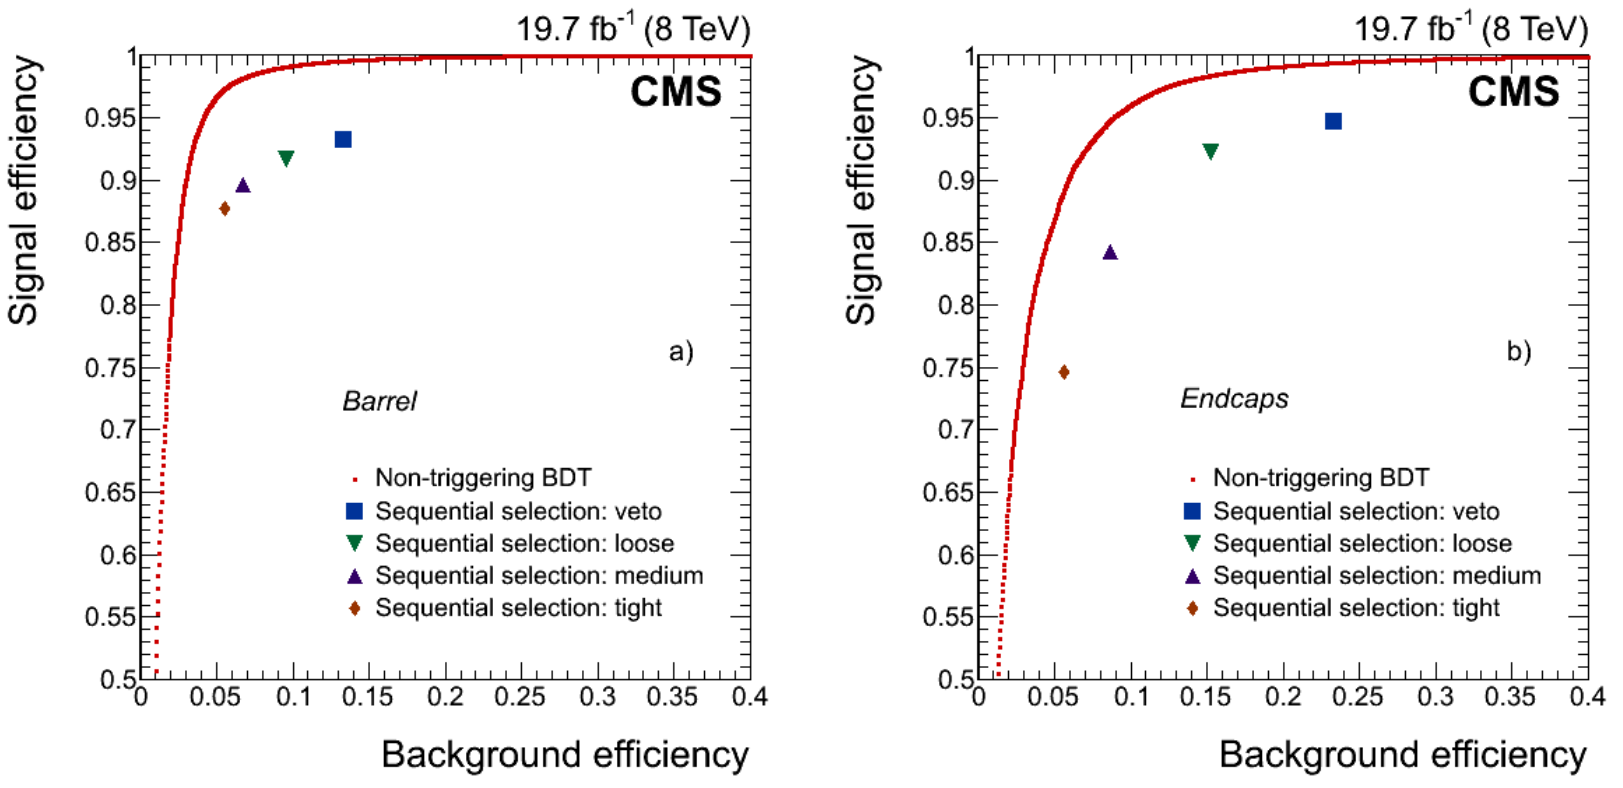
\includegraphics[width=0.95\textwidth]{plots_and_figures/chapter4/elec_eff.png}
\caption{Performance of the BDT-based electron identification algorithm (red dots) compared with results from several working points of cut-based selection for electron candidates in the ECAL barrel (left), and endcaps (right).}
 \label{fig:elec_eff}
\end{figure*}










\subsection{Jet Reconstruction}
\label{jet_recon}
Jets are clusters of particles that are experimental signatures of quark and gluons which hadronize (due to color confinement) producing a narrow spray or "jet" of particles. Jets are reconstructed in CMS from by clustering PF objects. In order to group together objects into a jet, CMS uses the anti-$k_{T}$ clustering algorithm. This belongs to a broader class of clustering algorithms called sequential clustering algorithms which cluster objects into jet in a sequential order following a predefined set of rules. The general form of a sequential clustering algorithm is based on the quantities  $d_{ij}$, which represents the distance between two entities, and $d_{iB}$ which represents the distance of the i-th entity from the beam axis. These distances are defined as:
\begin{equation*}
  d_{ij}=min(k_{ti}^{2p},k_{tj}^{2p})\frac{\Delta_{ij}^{2}}{R^2}
\end{equation*}
\begin{equation*}
  d_{iB}=k_{ti}^{2p}
\end{equation*}
where $\Delta_{ij}^{2}=(\eta_i-\eta_j)^2+(\phi_i-\phi_j)^2$, $k_{ti}$ is the transverse momentum of the i-th entity and R is the radius parameter which is set as 0.4. The parameter p governs the relative power of energy versus geometrical scales and the particular value of $p=-1$ defines the anti-$k_{T}$ clustering algorithm. The algorithm first computes distance $d_{ij}$ between all entity pairs present at that stage. If the minimum of those distances (say between entity i and j) is smaller than the minimum distance $d_{iB}$ of any entity from the beam axis, those entities i and j are combined into a single entity. Otherwise, the entity closest to the beam axis is considered a jet and removed from the list of entities to be further clustered. This continues until all entities are clustered. The anti-$k_{T}$ is dominated by high \pt particles which it clusters first subsequently including softer and softer constituents. Soft particles tend to cluster with hard particles before they tend to cluster among themselves. Hard particle has no hard neighbours within a distance 2R accumulate all the soft particles within a circle of radius R. It tries to produce jets with fairly conical shapes that are centered around the hardest particles of the event, and with boundaries that resilient to the effect of soft radiation.

Jets being complex objects suffer from several effects that cause there energy, reconstructed as described above, to differ from their true values. Multiplicative correction factors are applied to calibrate their \pt and to ensure a uniform response in $\eta$. A total of four multiplicative corrections are applied. Firstly, the energy coming from pileup that has been clustered into the jet needs to be corrected for. A correction is applied based on the \textit{hybrid jet area} method which is a combination of two methods viz., the average offset method and the jet are method. The average offset method uses zero bias events to measure the average amount of energy added to the event due to pileup. The assumption is that averaging over zero bias events makes this measurement insenstive to high \pt objects and primarily represents soft pileup contributions. The average offset is measured in bins of $\eta$ and number of pileup vertices ($N_{PV}$) averaged over $\phi$. The correction is then given by $1-\frac{<Offset(N_{PV},\eta)>}{p_{T}^{RAW}}$, where $p_{T}^{RAW}$  is the uncorrected jet \pt. The drawback of this method is that it assumes that every jet contains the same amount of pileup contribution. The jet area method, on the other hand , calculates corrections on a jet-by-jet basis. It calculates an energy density  per event  by clustering jets using the $k_{T}$ algorithm (this has a value of parameter p=1 and favours clustering soft jets as opposed to hard ones) and dividing the \pt by jet area, which is defined as the region in $\eta-\phi$ occupied by soft particles clustered in the jet. The median of this distribution for an event $\rho$ is expected to be insensitive to hard particles and thus $\rho A_{j}$ is a good approximation of pileup contribution to the i-th jet. The drawback of this second approach, however is that it doesn't take into account the fact that the detector response is $\eta$ dependent. The \textit{hybrid jet area} method combines these two methods to calculate a jet-by-jet correction depending on $\eta$ and $N_{PV}$. Secondly, a MC calibration factor, which corrects the energy of erconstructed jets to match the generated MC particle jet energy on average is applied. This factor is based on simulated events. Finally two Other factors are used that each calibrate the energy response to be uniform with respect to $\eta$ and \pt. These are also measured using simulated events.
%%%%FIXXXXXXXXXXXXXXXXXXXXXXX
The dependence on is measured using a QCD dijet sample in which two jets that are back to back in azimuthal angle are selected. Since these two jets will fall in di↵erent ⌘ regions and should have a sum of zero momentum in the transverse plane, they can be compared to determine a relative di↵erence in response based on region. This relative response is then used
40
to correct the jet energy to be flat versus ⌘. In order to correct for the response versus jet pT , samples of Z + jets and   + jets are used. These are chosen because the Z/  energy can be accurately measured as well as single jet recoiling from them. Again exploiting conservation of momentum in the transverse plane, the jet energy response can be calculated as a function of pT .
%%FIXXXXXXXXXXXXXXXXXXXXXXX 


\subsection{MET, MT and Collinear Mass}
\label{col_mass}
\subsection{Tau Lepton and others}
\label{tau_recon}


\section{Datasets}
\label{datasets}

The data analysed in this search was gathered by the CMS detector in 2016 during proton-proton collisions at the LHC, corresponding to an integrated luminosity of $35.9 fb^{-1}$. This data corresponds to a center-of-mass energy of 13 TeV and a spacing of 25ns between bunch crossings in the LHC with an average of about 30 collisions per bunch crossing. The subset of samples used among all collected by CMS are the ones having at least one isolated muon having transverse energy over 24 GeV, as triggered by the CMS high level isolated muon trigger (HLT\_IsoMu24 in CMS parlance).




% % uncomment the following lines,
% if using chapter-wise bibliography
%
% \bibliographystyle{ndnatbib}
% \bibliography{example}

% % uncomment the following lines,
% if using chapter-wise bibliography
%
% \bibliographystyle{ndnatbib}
% \bibliography{example}




%\chapter{Event Selection}
\label{evt_sel}
\epigraph{It is, indeed an incredible fact that what the human mind, at its deepest and most profound, perceives as beautiful finds its realization in external nature.… What is intelligible is also beautiful.}{\textit{Subrahmanyan Chandrasekhar}}
\vskip 0.5in
\section{Introduction}
\label{evt_sel_intro}
This chapter describes in detail the event selection criteria for the analyses, and how they were chosen. It starts by introducing the backgrounds that each of selection criterion is trying to reduce in order to get a higher ratio of number of signal events to background events, leading to a better sensitivity for the search. This is followed by the procedure for arriving at the best possible set of selection criterion. For the \hmue analysis, two methods of selection were developed. The first method developed involves placing requirements on several kinematic variables, and then using the resulting distribution of \mcol as discriminant for a binned likelihood fit (see section ~\ref{stat_meth} for description of statistical procedures). We call this method \mcol fit method. The second method developed involves using a Boosted Decision Trees (BDT) discriminator  for classification of signal and background events. The output distribution of the BDT discriminator is then used to perform the fit. We call this method BDT method. The BDT method is found to have greater sensitivity, as discussed later in the chapter. However, the \mcol fit method is also presented as a complementary method and acts like a cross-check for the BDT method. For \Hmue analysis, only the \mcol fit method is developed. This is in part due to the difficulties foreseen in training a BDT with much fewer events available in \Hmue analysis, and in part since this is the very first time the \Hmue search is being performed, a simpler analysis was felt to be adequate.  

Both analyses were performed blinded~\cite{blind_analysis} in the signal region. All selection criterion and methods described below were developed without the knowledge of the observed data in the range of variable spectra where the signal is expected to be present. This is considered an optimal way of eliminating the unintended biasing of a result in a particular direction and is a standard methodology in particle physics analyses. It is important to note here that the signal region is known for the $\hmue$ analysis. However, for the $\Hmue$ analysis, the signal region is presupposed - as there is no current evidence for H or its mass.

\section{h125: \hmue analysis}
\label{h125_evt_sel}
\subsection{\hmue: Final state signature and backgrounds}
\label{h125_signature}
The signature of the \hmue analysis final state consists of a muon that comes promptly from the Higgs and has a hard $\pt$ spectrum, along with a softer electron of opposite sign charge that comes from the tau lepton, and missing transverse momentum from the tau decay. It is interesting to note that the signature is similar to the $\text{h} \to \Pgt_{\Pgm}\Pgt_{\Pe}$ decay that is allowed by the SM and since been observed~\cite{CMS-PAS-HIG-16-043}, but with significant kinematic differences. In \hmue decay the $\Pgm$ comes directly from the Higgs resulting in its $\pt$ spectrum peaking and spreading out to much higher values. Also there are fewer neutrinos in \hmue, coming from the decay of the single $\Pgt$. The decay products of this highly boosted tau are closely aligned, leading to a narrow separation between the $\Pe$ and the $\ptvecmiss$ in the azimuthal plane. The same is not true in the $\text{h} \to \Pgt_{\Pgm}\Pgt_{\Pe}$ decays. These differences are illustrated pictorially in Fig.~\ref{fig:htt_v_lfv}.


\begin{figure*}
\begin{center}
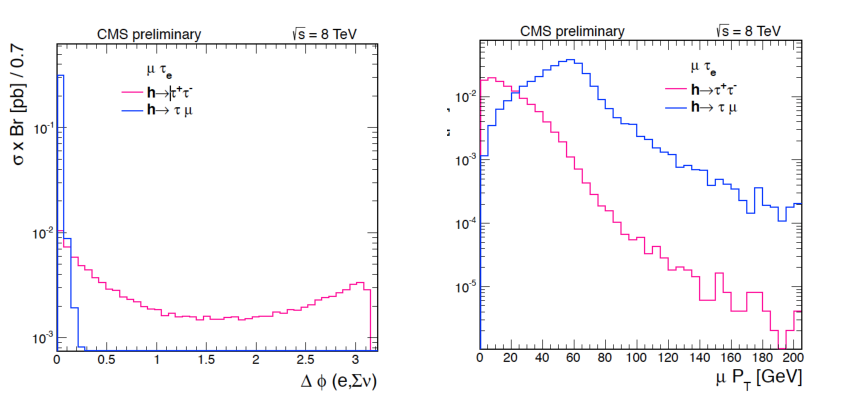
\includegraphics[width=0.8\textwidth,keepaspectratio]{plots_and_figures/chapter5/htt_v_lfv.pdf}
\caption{Illustration of the differences in $\pt^{\Pgm}$ and $\dphiemet$ spectrums in $\hmue$ and $\text{h} \to \Pgt_{\Pgm}\Pgt_{\Pe}$ processes.}
\label{fig:htt_v_lfv}
\end{center}
\end{figure*}

The most dominant backgrounds consists of \ztt events coming from Drell-Yan production and \ttb production. In \ztt events, one $\Pgt$ can decay to an $\Pe$ and the other to a $\Pgm$. This background peaks at lower values of $M_{col}$ than the signal events but there is significant overlap with the signal spectrum. In \ttb production, each of the top quarks can decay into a bottom and a $\PW$ with the $\PW$ bosons then decaying to a $\Pe$ and $\Pgm$. The other backgrounds are smaller and include (in no particular order) electroweak diboson production ($\PW\PW$, $\PW\PZ$ and $\PZ\PZ$), h boson decays allowed by the SM ($\PH \to \Pgt\Pgt,\PW\PW$), $\PW\gamma^{(*)}+\text{jets}$ ,single top production, \wjets events, $Z\to\ell\ell$ $(\ell = \Pe, \Pgm)+\text{jets}$ and QCD multijet backgrounds. These backgrounds are described in more detail, along with there estimation and validation techniques in section~\ref{bg_val}.        


\subsection{\hmue: Baseline selection and categorization}
\label{h125_presel_cat}
A baseline selection is defined first in order to ensure that we have clean and well-defined events faithful to the final state signature of the signal process. An isolated and well-identified $\Pgm$ is thus required to be present along with a well-identified and isolated $\Pe$ of opposite sign charge. They are required to be separated by $\Delta R > 0.3$. The identification criterion applied for $\Pgm$ and $\Pe$ have been described in sections~\ref{mu_recon} and~\ref{e_recon}. Isolation criterion, as measured by $I_\text{rel}$ (described in ~\ref{tau_recon}), are required to have values $I_\text{rel}^{\Pe} < 0.15$ and $I_\text{rel}^{\Pgm} < 0.1$. The $\pt$ of these candidates are required to be above minimal thresholds required by trigger, identification and isolation requirement. Both candidates are also required to be within the fiducial region of the detector. The $\Pgm$ is required to have $\pt^{\Pgm} > 26$\GeV and $|\eta^{\Pgm}|<2.4$.The $\Pe$ is required to have $\pt^{\Pe} > 10$\GeV and $|\eta^{\Pe}|<2.3$. Only events with two or fewer jets are considered. All jets considered must have $\pt>30$\GeV, $|\eta| < 2.4 $ and satisfy the loose identification criterion described in section~\ref{jet_recon}. Events with one or more jets arising from a b-quark (b-tagged jets) are vetoed. Cleaning events with b-tagged jets reduce some contribution from backgrounds which give rise to b-quarks such as \ttb and single top. Also, as described in~\ref{jet_recon}, any event with one or more jets within $\Delta R < 0.4$ of either lepton candidates is also rejected. Further, an event is rejected if it has additional $\Pgm$ or $\Pe$, or any $\Pgt_{had}$ candidates. All the above baseline selection requirements have been summarized in Table~\ref{tab:h125_base_sel}. All the events were required to pass isolated muon triggers with a $\pt$ threshold of 24 \GeV. The trigger selection has been described in detail in section~\ref{trigger}. The distributions of the \mcol and several other kinematic variables after the baseline selection just described, are shown in Figs.~\ref{fig:h125_presel1} and ~\ref{fig:h125_presel2}. These distributions act as the starting point for development of stricter kinematic selections looking at the different shapes of signal and backgrounds distributions for different variables.     


\begin{table}[htpb]
 \begin{center}
 \caption{Baseline selection criteria for \hmue analysis}
  \begin{tabular}{c|c|c} \hline
    Variable    &  $\Pgm$  & $\Pe$ \\ \hline
    $\pt $       & $>30$\GeV &  $>10$\GeV                                           \\
    $|\eta| $       & $<2.4 $ &  $<2.3$                                           \\
    $I_{\text{rel}}$  & $<0.15$ &  $<0.1$                                           \\
    \multicolumn{3}{c}{Cleaning requirements} \\\hline
    \multicolumn{3}{c}{ $\Delta R(\Pgm,\Pe) > 0.3$} \\ 
    \multicolumn{3}{c}{No additional $\Pgm$, $\Pe$ or $\Pgt_{had}$} \\
    \multicolumn{3}{c}{No b-tagged jets with $\pt>30$\GeV} \\
    \multicolumn{3}{c}{No jets with $\Delta R(\Pgm,jet)<0.4$ and $\pt>30$\GeV} \\
    \multicolumn{3}{c}{No jets with $\Delta R(\Pe,jet)<0.4$ and $\pt>30$\GeV }\\
    \hline
  \end{tabular}
  \label{tab:h125_base_sel}
  \end{center}
\end{table}


\begin{figure*}[!htpb]\centering
 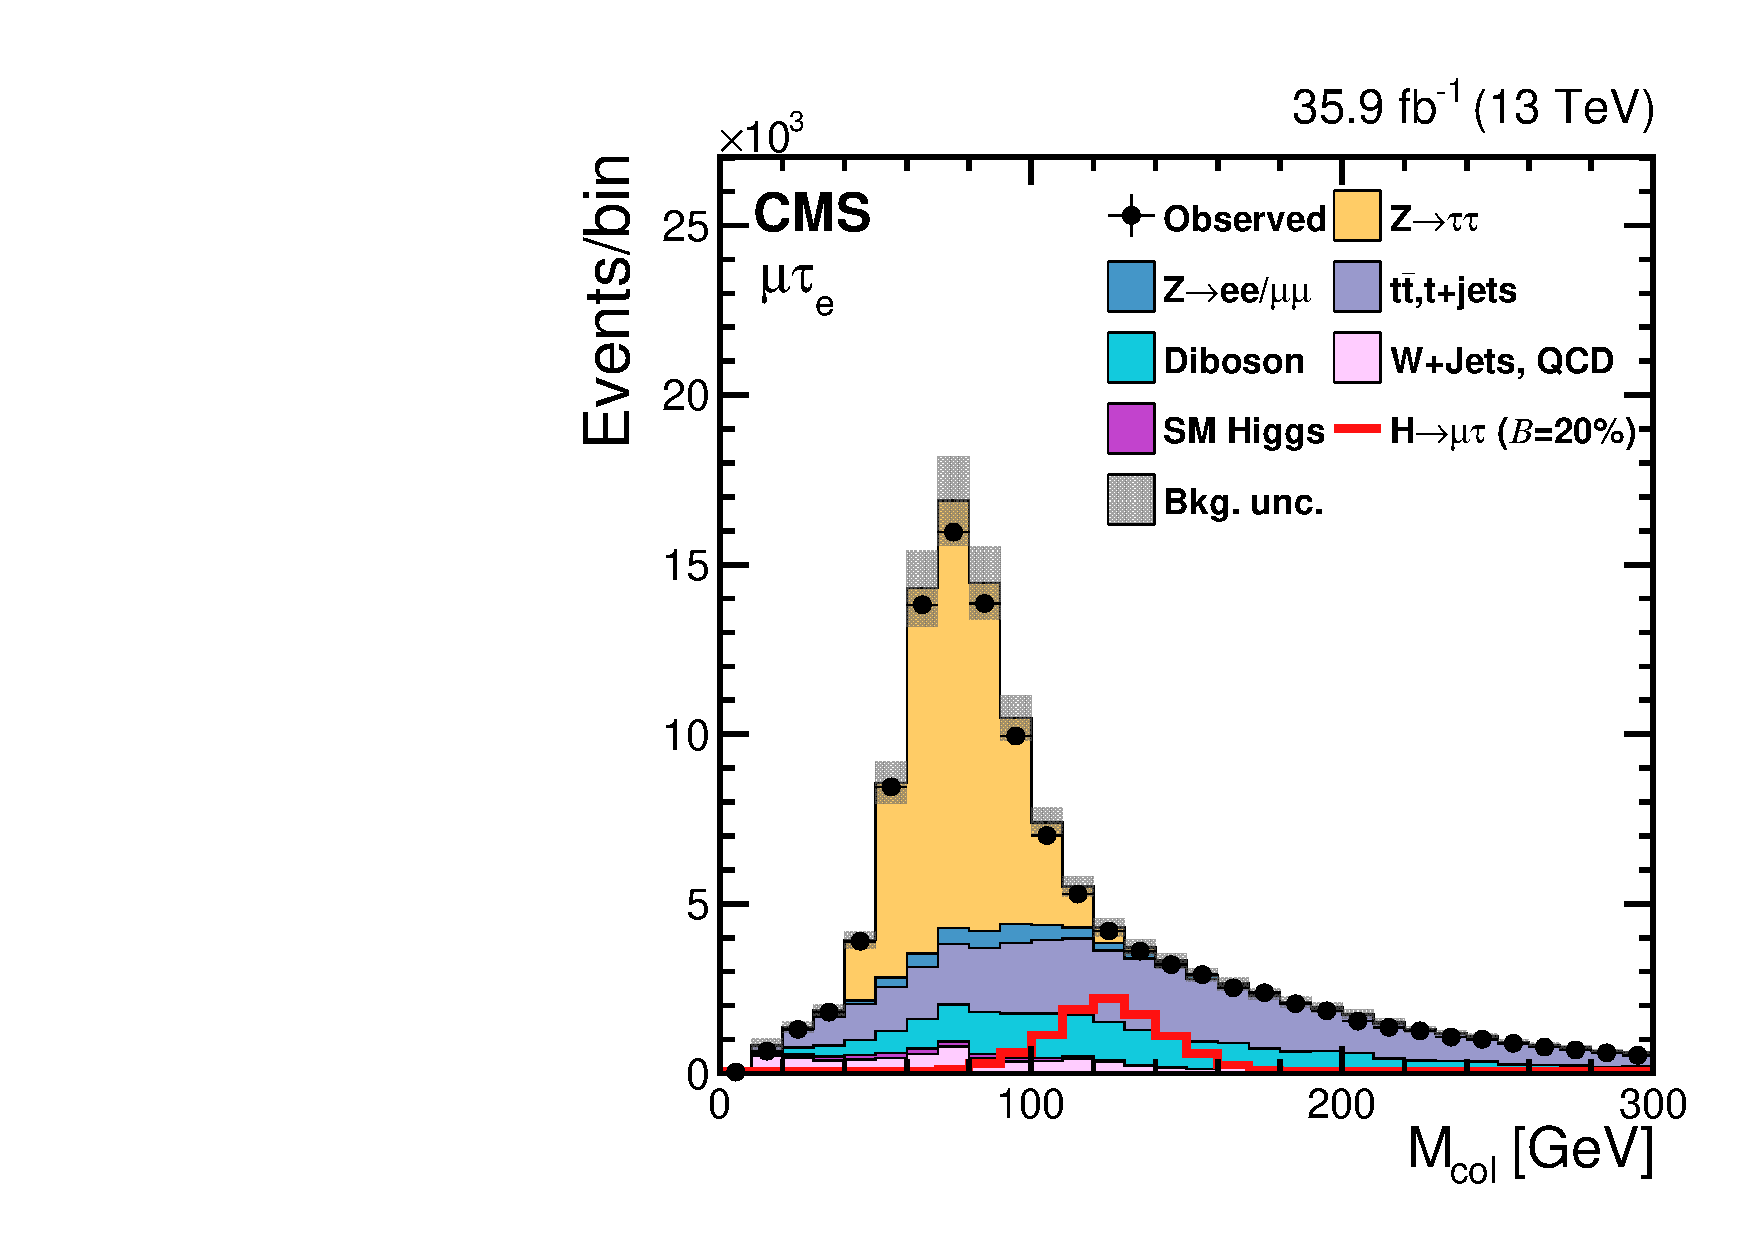
\includegraphics[width=0.49\textwidth]{plots_and_figures/chapter5/preselection/Figure_002-a.pdf}
 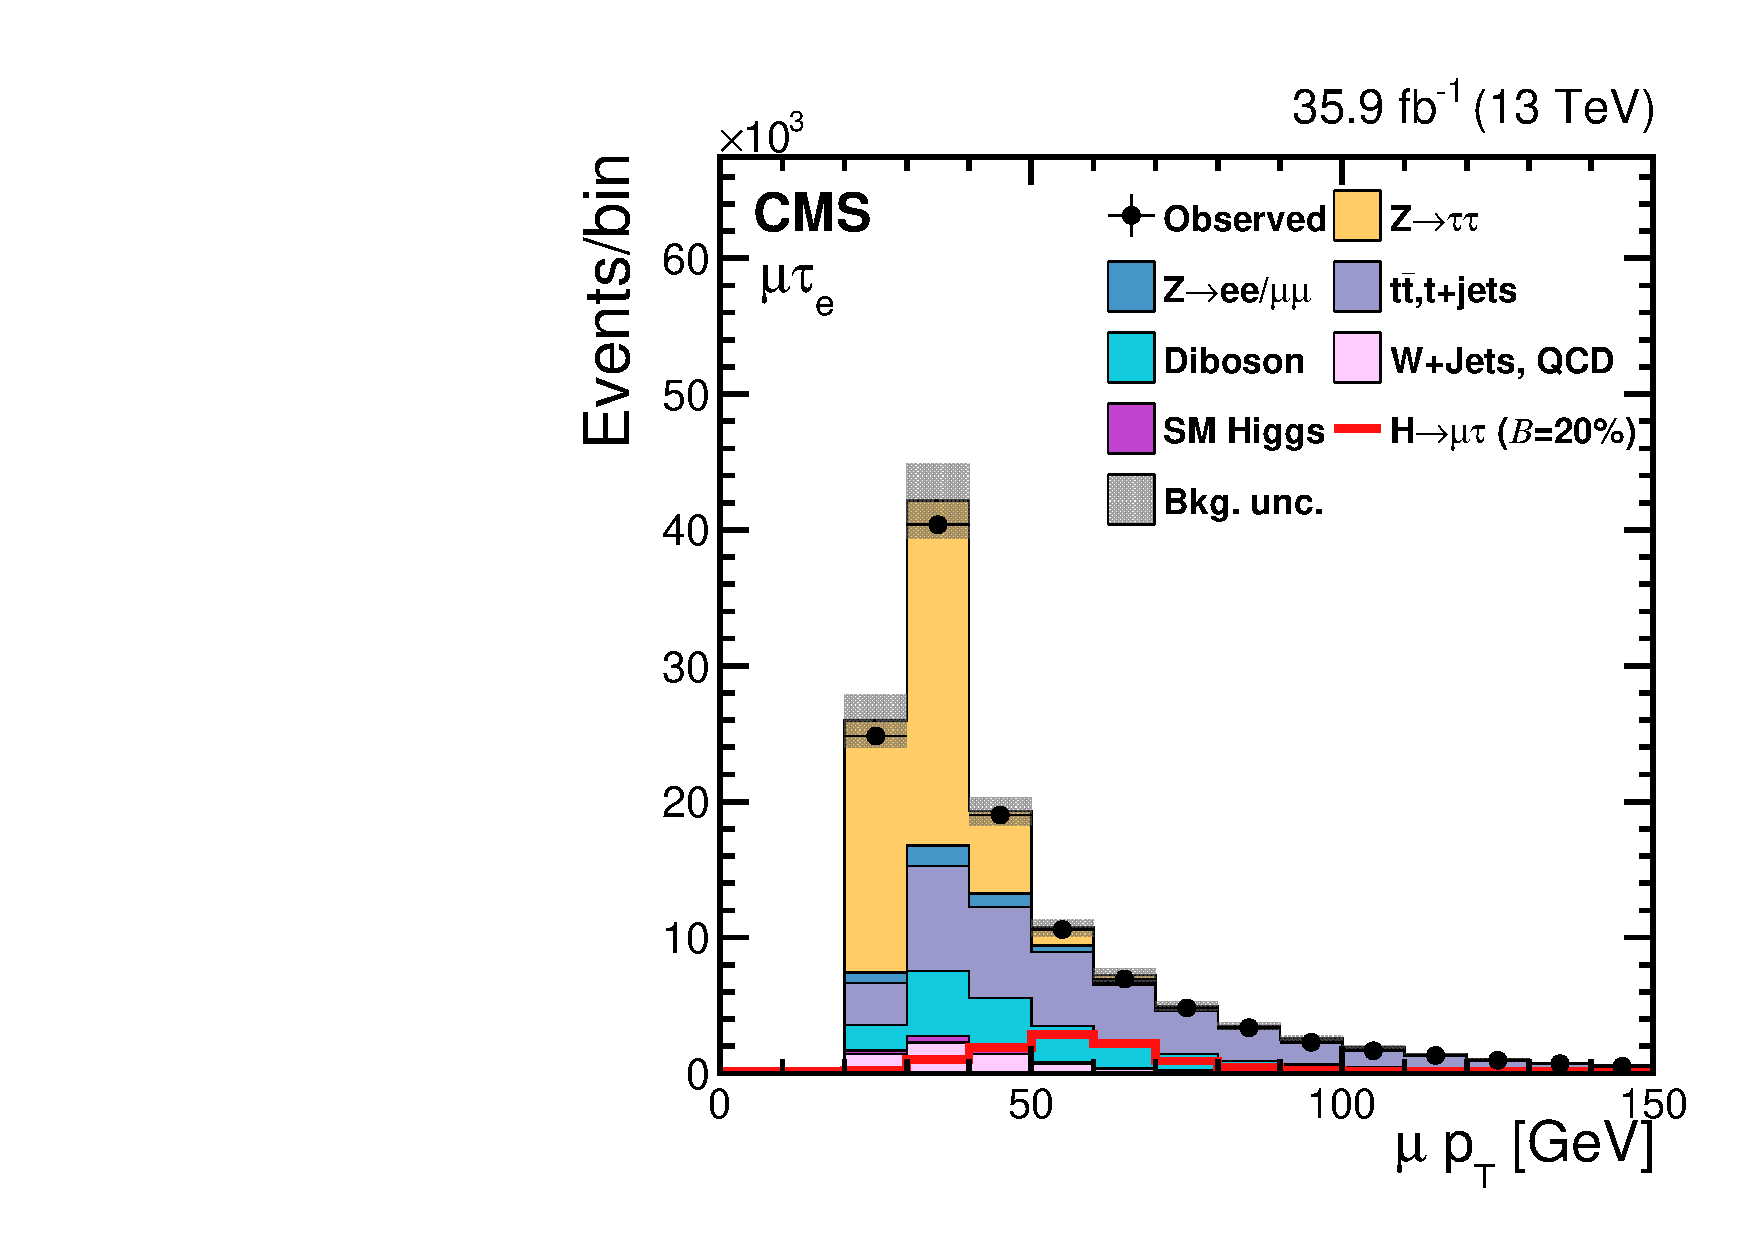
\includegraphics[width=0.49\textwidth]{plots_and_figures/chapter5/preselection/Figure_002-b.pdf} \\
 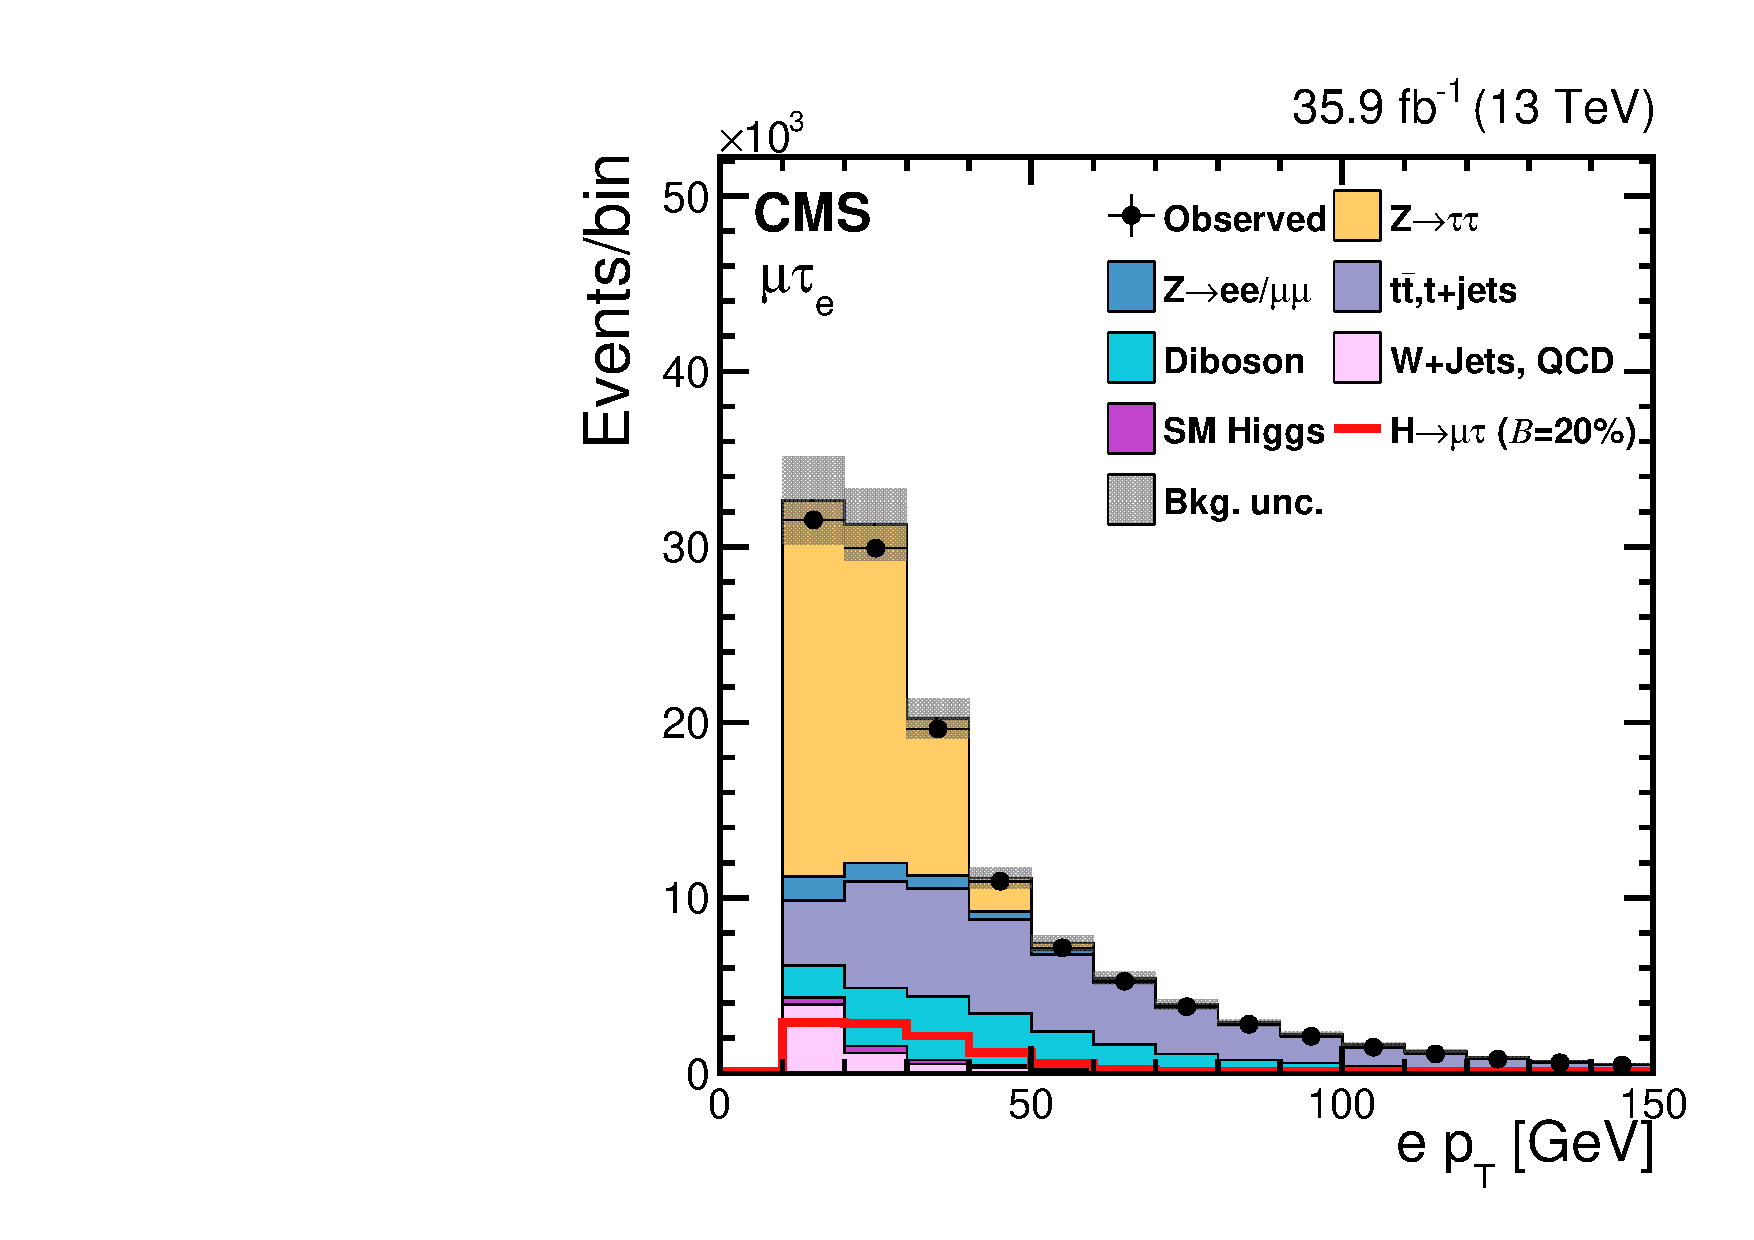
\includegraphics[width=0.49\textwidth]{plots_and_figures/chapter5/preselection/Figure_002-c.pdf}
 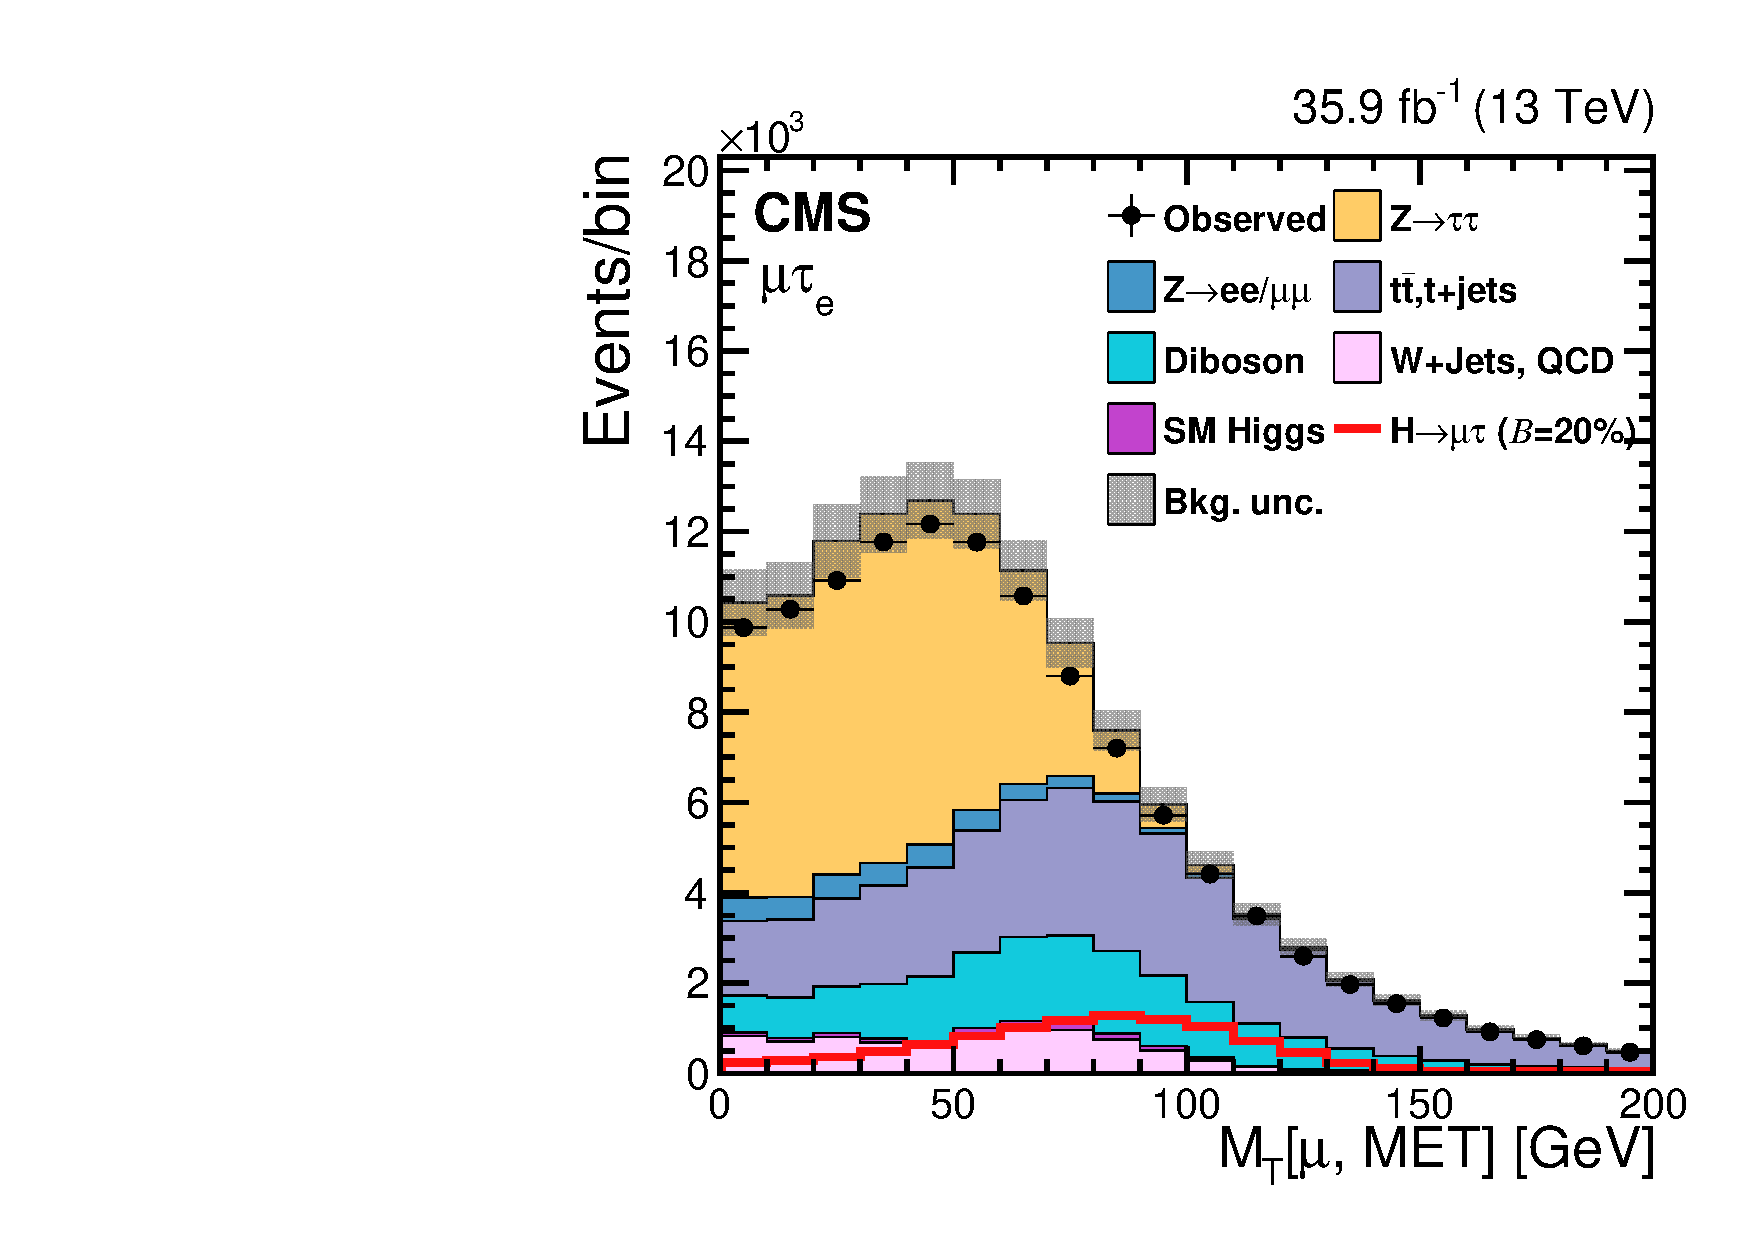
\includegraphics[width=0.49\textwidth]{plots_and_figures/chapter5/preselection/Figure_002-d.pdf} 
\caption{Distributions of kinematic variables after baseline selection for \hmue analysis (1).}
 \label{fig:h125_presel1}
\end{figure*}
\begin{figure*}[!htpb]\centering
 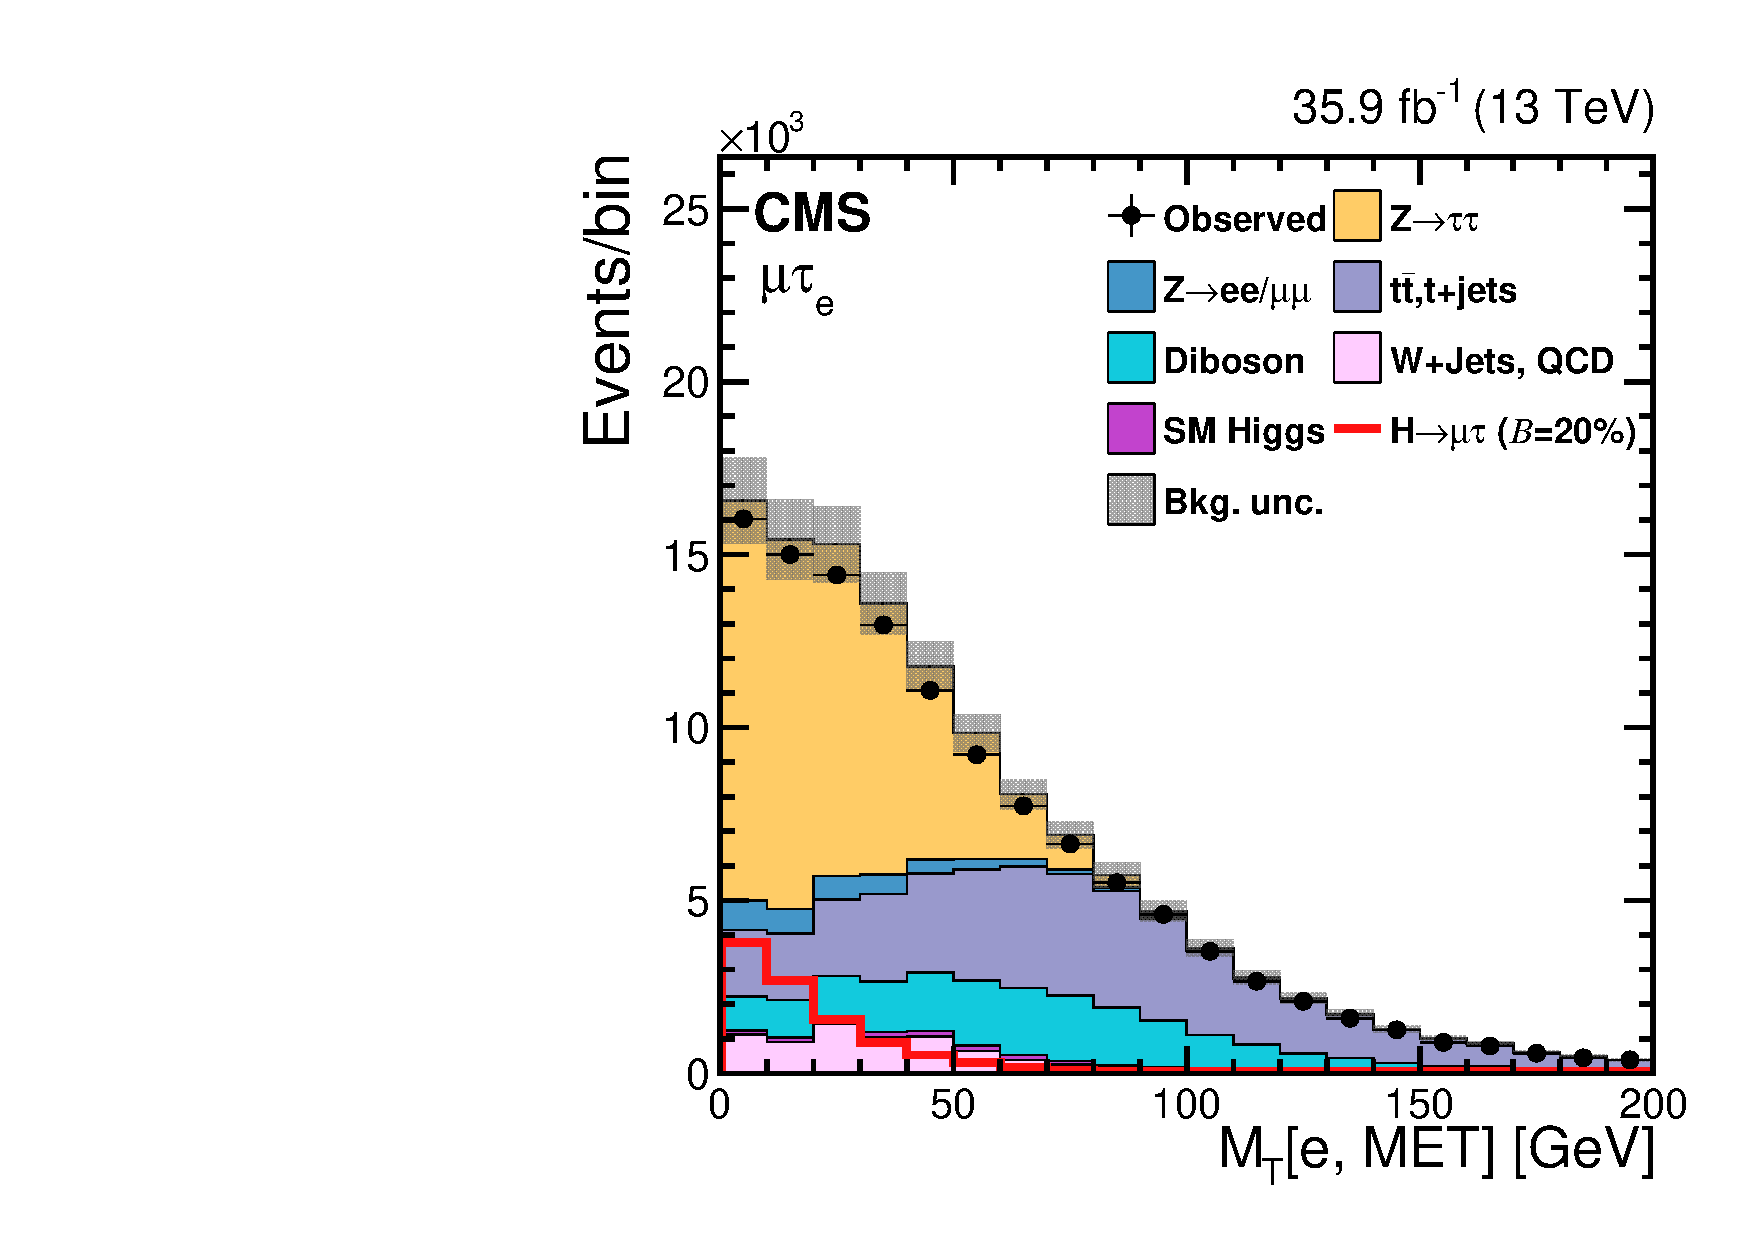
\includegraphics[width=0.49\textwidth]{plots_and_figures/chapter5/preselection/Figure_002-e.pdf}
 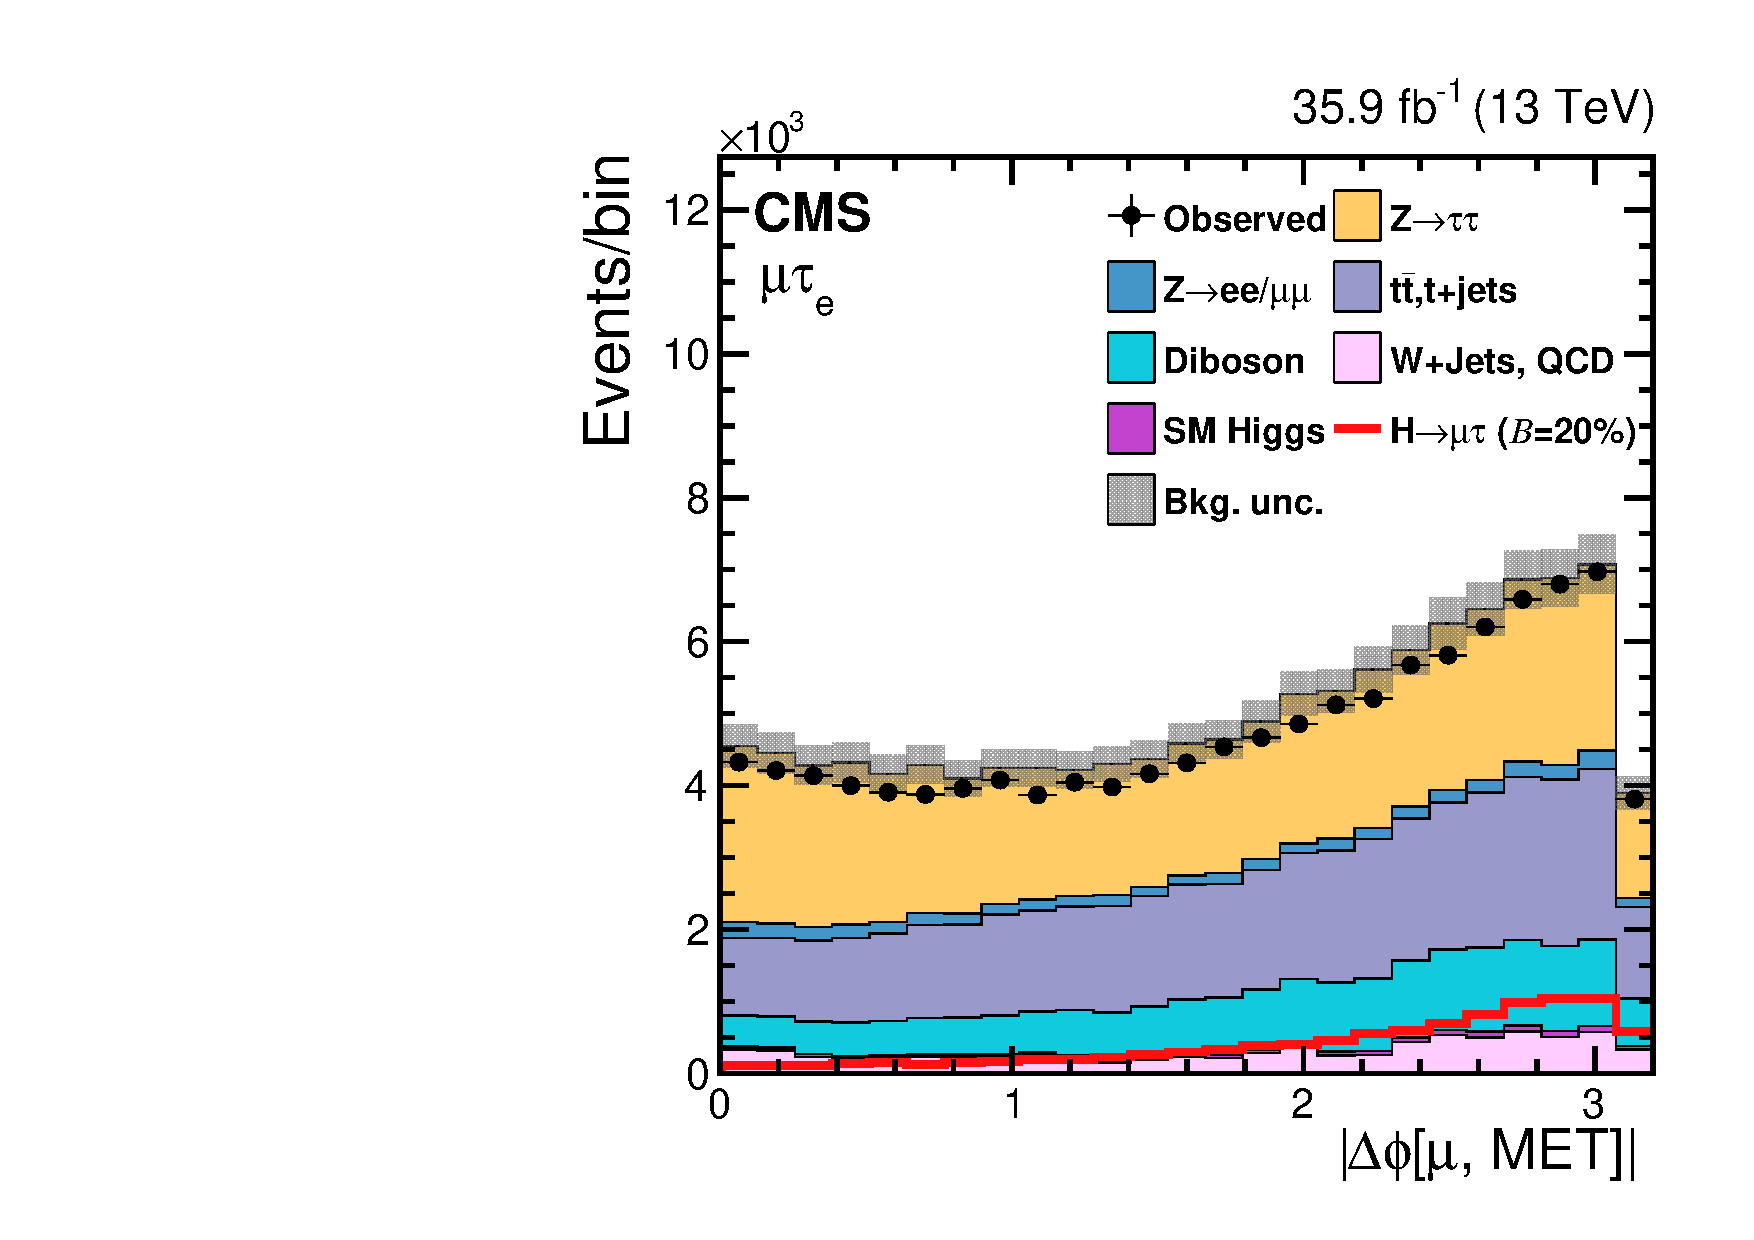
\includegraphics[width=0.49\textwidth]{plots_and_figures/chapter5/preselection/Figure_002-f.pdf} \\
 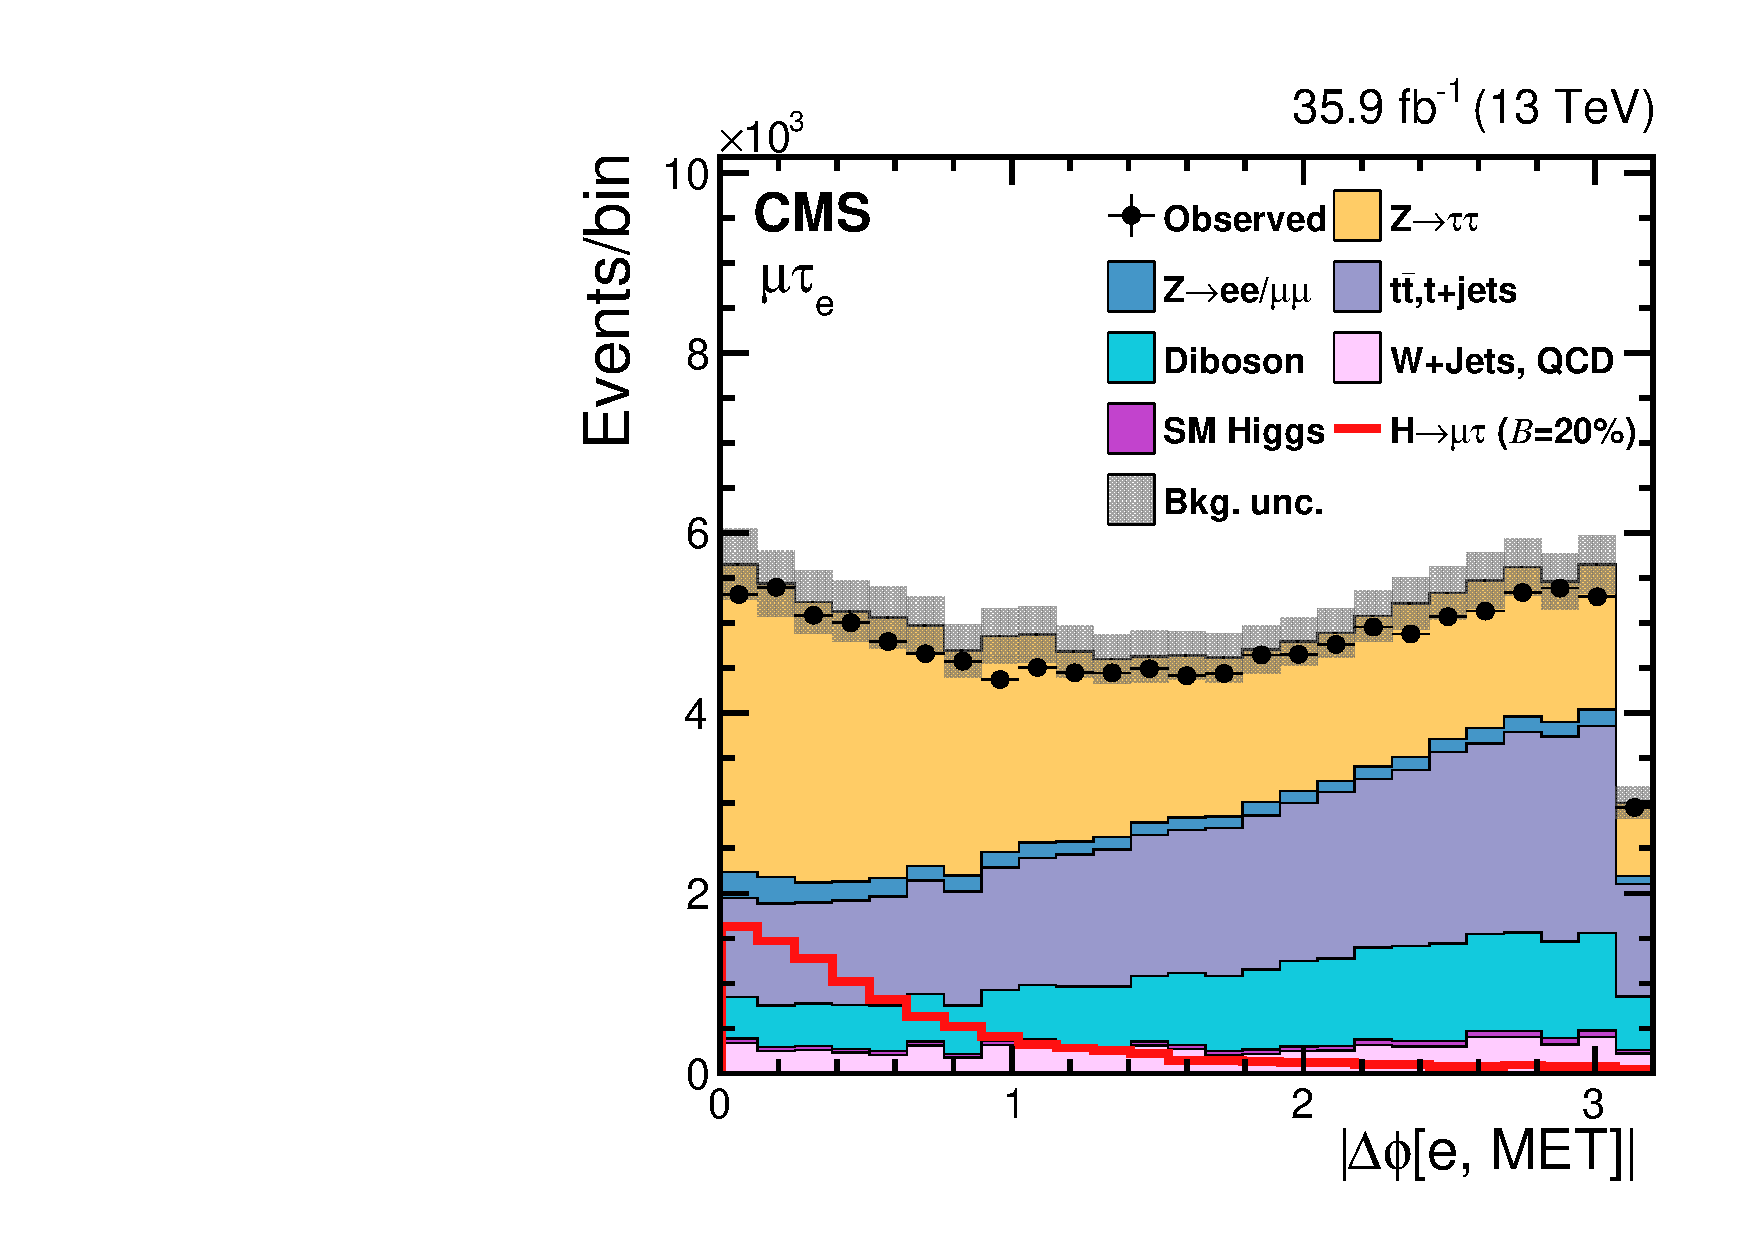
\includegraphics[width=0.49\textwidth]{plots_and_figures/chapter5/preselection/Figure_002-g.pdf}
 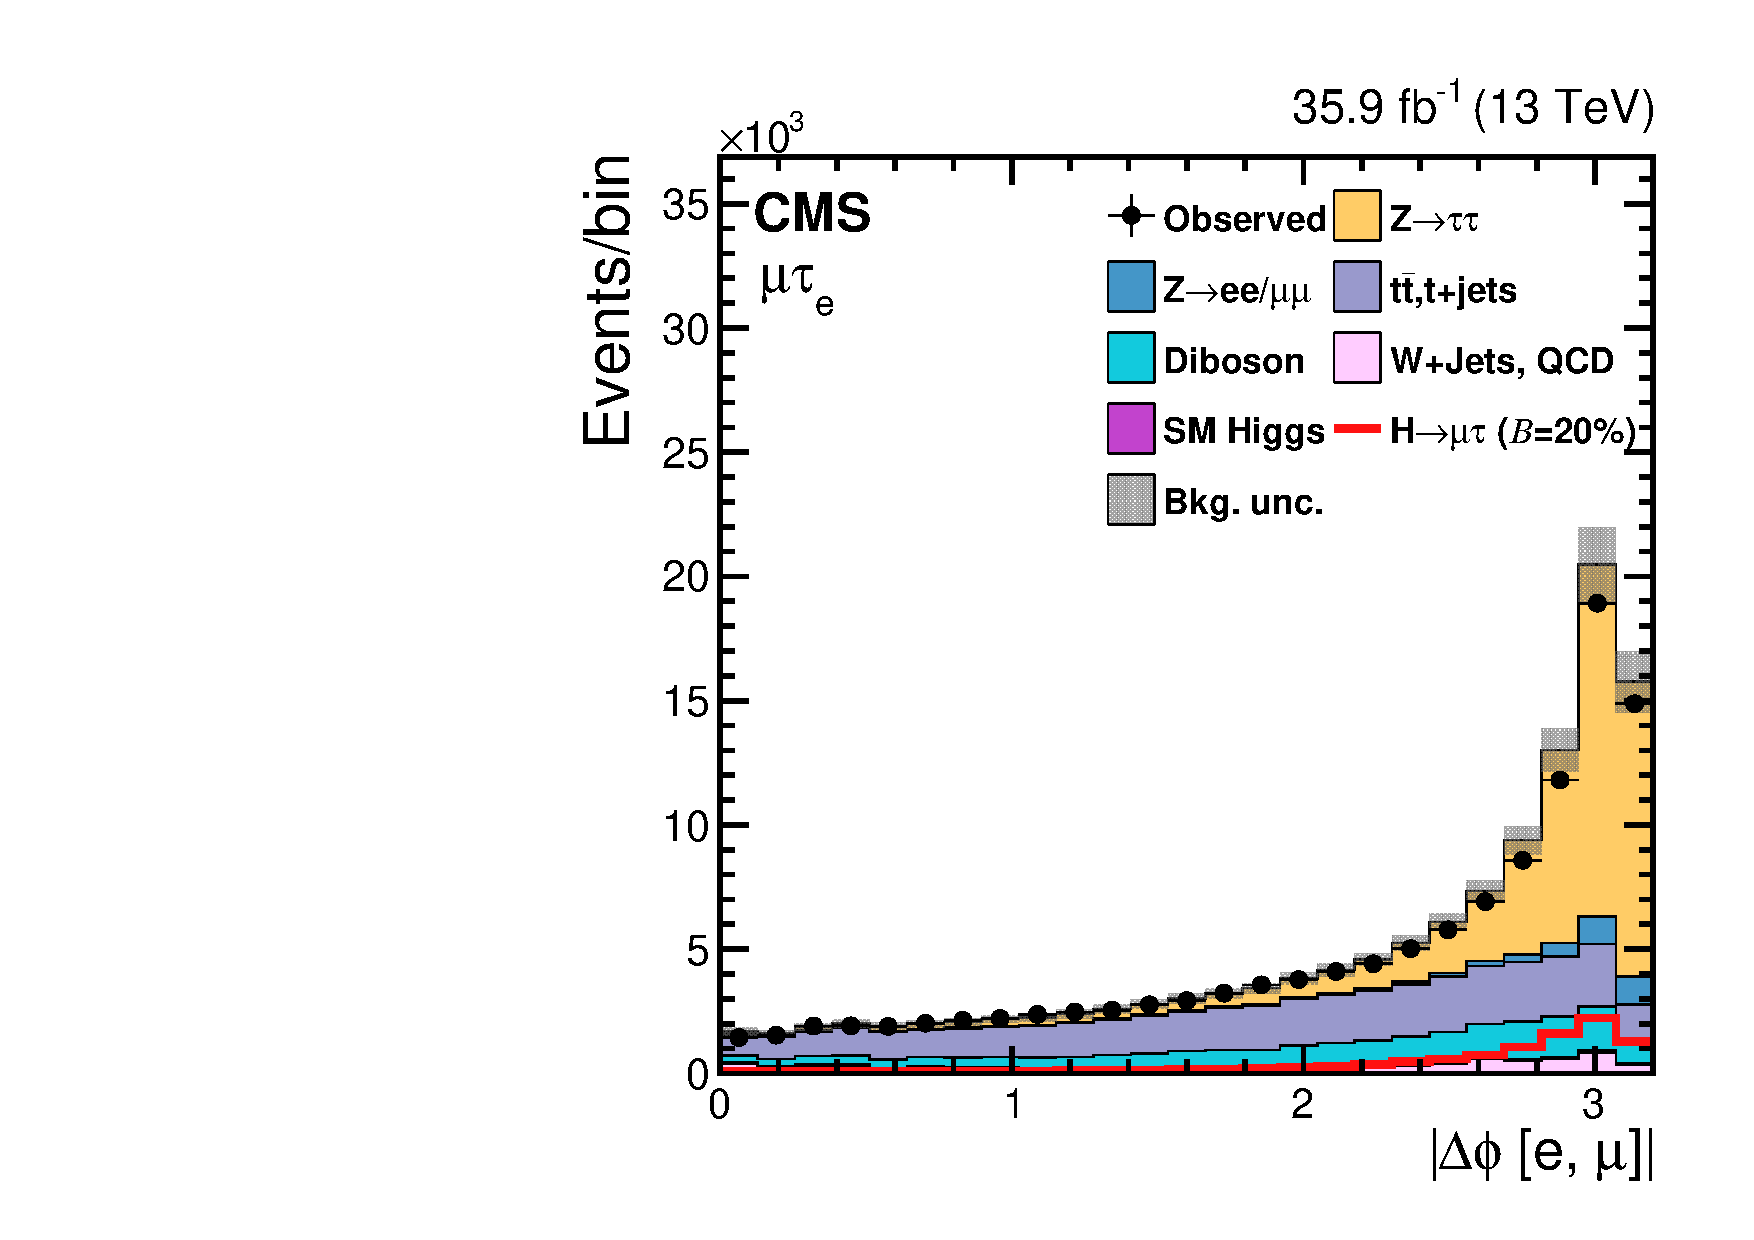
\includegraphics[width=0.49\textwidth]{plots_and_figures/chapter5/preselection/Figure_002-h.pdf}
\caption{Distributions of kinematic variables after baseline selection for \hmue analysis (2).}
 \label{fig:h125_presel2}
\end{figure*}

At this point the events are divided into several buckets, called categories. This is done on the basis of number of jets present in the event. In events with 2 jets the invariant mass of the di-jet system ($M_{jj}$) is also used for categorization. The topology of events containing different number of such jets can be different. For example, in events with one energetic jet the h produced can be boosted resulting in the azimuthal separation of the $\Pgm$ and $\Pe$ (that come from its decay) to be narrower than events with no jets. Each of this categories enhance the contribution of different h boson production mechanisms, and requiring different optimal selection criteria in each category  helps increase the sensitivity of the search. The categories in order of decreasing number of signal events are:
\begin{itemize}
\item \textbf{0-jet category}: These are events that do not have any jet. This category enhances the gluon-gluon fusion (GGF) contribution.
\item \textbf{1-jet category}: Events that have 1 jet are put in this category. This category enhances the GGF production with initial state radiation (ISR). Some VBF events where one jet has escaped detection can also enter this category.
\item \textbf {2-jet GGF category}: This category contains events that have 2 jets with the additional requirement that $M_{jj}<550$\GeV. The dominant contribution comes from GGF production in association with two jets.
\item \textbf{2-jet VBF category}: This category contains events that have 2 jets with the additional requirement that $M_{jj}\geq 550$\GeV. The dominant contribution comes from VBF production which is characterized by presence of two jets with high dijet mass.  
\end{itemize}

\subsection{\hmue: \mcol fit selection}
\label{h125_cb_sel}
In the \mcol fit method, the selection is performed by placing kinematic cuts on several variables to enhance the signal-to-background ratio. There are several variables considered for this and they include: the azimuthal separation ($\Delta\phi$) between $\Pgm$ and $\Pe$, between $\Pe$ and $\ptvecmiss$, between $\Pgm$ and $\ptvecmiss$, denoted respectively by $\dphiemu$, $\dphiemet$, $\dphimumet$ , and the transverse mass between $\Pgm$ and $\ptvecmiss$, between $\Pe$ and $\ptvecmiss$, denoted respectively by $M_T(\Pgm)$ and $M_T(\Pe)$. The \hmue decay being a 2-body decay, the $\Pgm$ and $\Pe$ are expected to be well separated in the azimuthal plane. Therefore, selecting events with a $\dphiemu$ larger than a threshold can help reject background events while keeping the signal that is peaked at high $\dphiemu$ values. This can be seen from Fig~\ref{fig:h125_presel2} (bottom right). Both neutrinos in the signal process come from the decay of the same $\Pgt$. These neutrinos form the $\ptvecmiss$. As mentioned earlier, the $\Pgt$ being much lighter than the h, it is highly boosted and its decay products i.e. $\Pe$ and the $\ptvecmiss$ are expected to be close to each other in the azimuthal direction. Thus $\dphiemet$ is expected to peak at values close to zero for signal events, as seen in Fig~\ref{fig:h125_presel2} (bottom left). Given that all backgrounds have relatively flat shape for this variable  throughout the $\Delta\phi$ range, requiring $\dphiemet$ to be lower than a threshold works as a strong rejection criterion against the backgrounds. Following a similar line of reasoning, the $\Pgm$ is expected to be well separated from the $\ptvecmiss$ resulting in $\dphimumet$ for signal events to peak at high values, as seen in Fig~\ref{fig:h125_presel2} (top right). Further, as the $M_T(\ell)$ (defined in section ~\ref{col_mass}) contains negative of the cosine of $\Delta\phi(\ell, \ptvecmiss)$ term, it is expected to be peak at values similar to $\Delta\phi(\ell, \ptvecmiss)$. This can be seen from Fig ~\ref{fig:h125_presel2} (top left) and Fig~\ref{fig:h125_presel2} (bottom right) which show signal events for $M_T(\Pgm)$ and $M_T(\Pe)$ peak at relatively higher and lower values than most backgrounds respectively. In particular, requiring $M_T(\Pgm)$ to be larger than a threshold can help reject a lot of \ztt events which is the most dominant background in the 0-jet category. All the above variables have some amount of correlation with one another (see the correlation matrix shown in Fig.~\ref{fig:bdt_corr_mat}). The optimization procedure used to arrive at the most optimal set of kinematic thresholds for these variables is described in detail in the next paragraph. The thresholds on the $\pt$ of the $\Pgm$ and $\Pe$ have not been made stricter to avoid biasing the selection toward energetic leptons that sculpt the background $\mcol$ distribution to mimic the signal peak. This effect could potentially reduce the shape discrimination power of the signal extraction procedure. Only in the 0-jet category category the requirement on $\pt$ of the $\Pgm$ is made marginally stricter by requiring  $\pt^{\Pgm} > 30$\GeV. All other lepton $\pt$ requirements are allowed to remain the same as baseline selection and are not included in the optimization procedure.   

The aim of the optimization procedure is to maximize the sensitivity of the analysis. In other words, we want to select a set of thresholds which increases a quantity such as the $\frac{S}{\sqrt{S+B}}$ ratio where S and B are the number of estimated signal and background events respectively. It is also necessary to ensure along-with, that the entire spectrum of distribution of the discriminant variable (that is used in the final max-likelihood fit to extract results) is well-populated, especially in the region where the signal is expected to appear. A bad fit can potentially degrade the sensitivity of the analysis. Taking both of the above points into consideration, the thresholds have been optimized to obtain the most stringent (lowest) possible expected limits. The definition and procedure of extracting the expected limit is given in section~\ref{exc_cal}. To do the optimization of the kinematic thresholds, we start by requiring the baseline selection. Then for a variable in consideration, e.g.- $\dphiemet$, we look at the expected limit while making the threshold progressively stricter until we reach a point where making the threshold any stricter degrades (increases) the expected limit. We repeat this procedure for all variables and note the stringent expected limit for each (by tightening thresholds of only that variable). This concludes one round of the optimization. For the next round we start by requiring the baseline selection. In addition we require that the variable that achieved the best possible expected limit among all variables in the last round satisfy its corresponding threshold. Lets call this variable variable1. We now repeat the same procedure as the last round for all but variable1. Say the variable that gave us the best possible expected limit this round is variable2. For the start of the following round variable2 is is required to satisfy its corresponding threshold. Then all the other variables (including variables that were had chosen thresholds in earlier rounds such as variable1 here) are made to go through the same procedure. This is done because the optimum value of threshold for variables chosen earlier might shift as new variables are chosen. This process is continued until the expected limit becomes no further stringent in successive rounds. This optimization was done separately for each of the four categories. The final set of thresholds arrived at in this way for the \hmue \mcol fit analysis are listed in Table.~\ref{tab:h125_sel_cuts}. This method of choosing the optimal set of thresholds is sometimes called the n-1 procedure, and the idea is conceptually similar to forward/backward selection methods used in statistical learning to build optimal models.             


\begin{table}[htpb]
 \begin{center}
 \caption{Final selection criteria for \hmue \mcol fit analysis}
  \begin{tabular}{c|c|c|c|c} \hline
    Category     &  0-jet    & 1-jet & 2-jet GGF & 2-jet \\ \hline
    $\pt^{\Pgm}$ & $>30$\GeV &  --   & --        & --     \\
    $M_T(\Pgm)$  & $>60$\GeV & $>40$\GeV & $>15$\GeV & $>15$\GeV \\
    $\dphiemet$  & $<0.7$ & $<0.5$ & $<0.3$ & $<0.3$ \\
    $\dphiemu$   & $>2.5$ & $>2.0$ & -- & -- \\
    
    \hline
  \end{tabular}
  \label{tab:h125_sel_cuts}
  \end{center}
\end{table}
\subsection{\hmue: BDT method selection}
\label{h125_bdt_Sel}
In the BDT method, a boosted decision trees (BDT) classifier is used to discriminate signal events from background events. A decision tree is a classifier which works by building a tree structure based on binary splits (as shown in Fig.~\ref{fig:dec_tree}). Starting from the root node of the tree (which contains all the events which we want to classify), a sequence of binary splits is made using input variables provided to the classifier. At each split, the variable which provides best purity of split or equivalently, in our case the best separation of signal and background events, is used. The same variable can thus be used for splitting several nodes and the splitting is continued until a desired stopping criterion such as depth of the tree, purity of leaf nodes, minimum number of events in a leaf node etc. is reached. All events end up in one of the leaf nodes. If an event ends up in a leaf node in which signal events form the majority fraction, it is classified as a signal event. Otherwise, it is classified as a background event. Boosting is a class of ensemble machine learning techniques which help in enhancing performance of weak classifiers by sequentially building classifiers using reweighted (boosted) versions of the training data and then taking a weighted majority vote of the sequence of classifiers thus produced. Boosting also stabilizes the response of the classifiers with respect to fluctuations in the training data. In other words it helps avoid overfitting to the training data. When the boosting technique is a applied to produce an ensemble of decision trees, the resulting ensemble of classifiers is called a Boosted Decision Trees classifier.

%A detailed overview of how decision trees and boosting works, and the chosen value of parameters used in training the BDTs for this analysis is given in appendix~\ref{chap_BDT}.

\begin{figure*}
\begin{center}
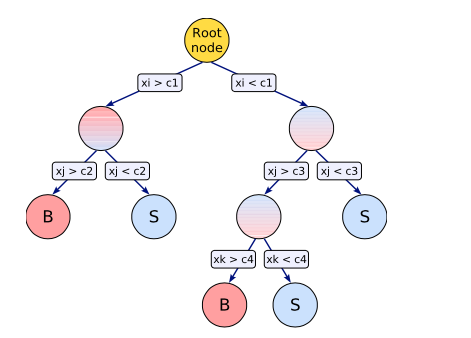
\includegraphics[width=0.8\textwidth,keepaspectratio]{plots_and_figures/chapter5/decision_tree.png}
\caption{Illustration of decision tree~\cite{tmva_manual}.}
\label{fig:dec_tree}
\end{center}
\end{figure*}


The BDT is trained using events that satisfy the baseline selection criteria. Simulated GGF and VBF events weighted by their cross-section are used as signal events for training. For background, a mixture of \ttb and Drell-Yan events are used, also weighted by their respective cross-sections. The \ttb and Drell-Yan backgrounds are the most dominant backgrounds. The Drell-Yan background is the most dominant background in 0-jet and 1-jet category, while the \ttb background is the most dominant in both 2-jet categories. It also has many kinematic characteristics in common with diboson and single-top backgrounds. A suite of input variables is used in training of the BDT. They are as follows:
\begin{itemize}
\item Transverse mass between the $\Pgm$ and $\ptvecmiss$: $M_T(\Pgm)$.
\item Transverse mass between the $\Pe$ and $\ptvecmiss$: $M_T(\Pe)$. 
\item Azimuthal angle between the $\Pe$ and $\Pgm$: $\dphiemu$. 
\item Azimuthal angle between the $\Pe$ and $\ptvecmiss$: $\dphiemet$.
\item Azimuthal angle between the $\Pgm$ and $\ptvecmiss$: $\dphimumet$. 
\item Collinear mass: \mcol.
\item Muon \pt: $\pt^{\Pgm}$. 
\item Electron \pt: $\pt^{\Pe}$.
\end{itemize}
The distributions of these variables normalized to the total number of events in the input sample to the BDT is shown in Fig.~\ref{fig:bdt_inp_var}. The correlations between these variables in signal and background events are shown in Fig.~\ref{fig:bdt_corr_mat}.
\begin{figure*}
\begin{center}
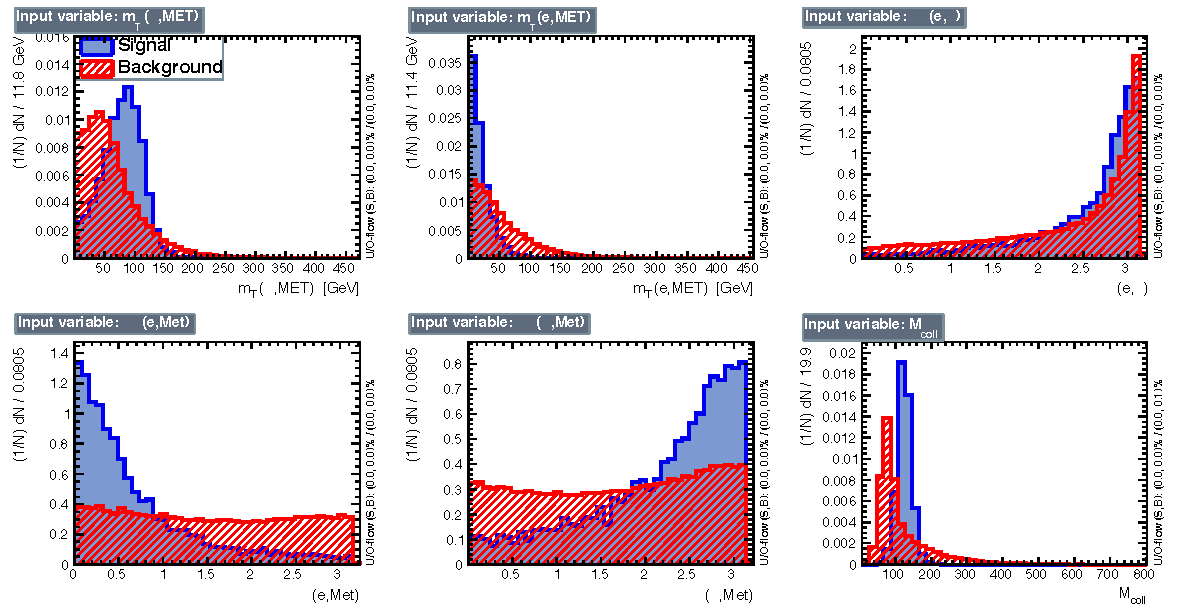
\includegraphics[width=0.9\textwidth]{plots_and_figures/chapter5/variables_id_c1.pdf}\\

\includegraphics[width=0.8\textwidth]{plots_and_figures/chapter5/variables_id_c2.png}\\
\end{center}
\caption{ Normalized distributions of the input variables for BDT method. The signal (blue) is composed of a weighted mixture of GGF and VBF events, whereas the background (red) is made of $t\bar{t}$ and Drell-Yan events. All events were required to satisfy the baseline selection criteria.}
\label{fig:bdt_inp_var}
\end{figure*}

\begin{figure*}[htpb]
\begin{center}
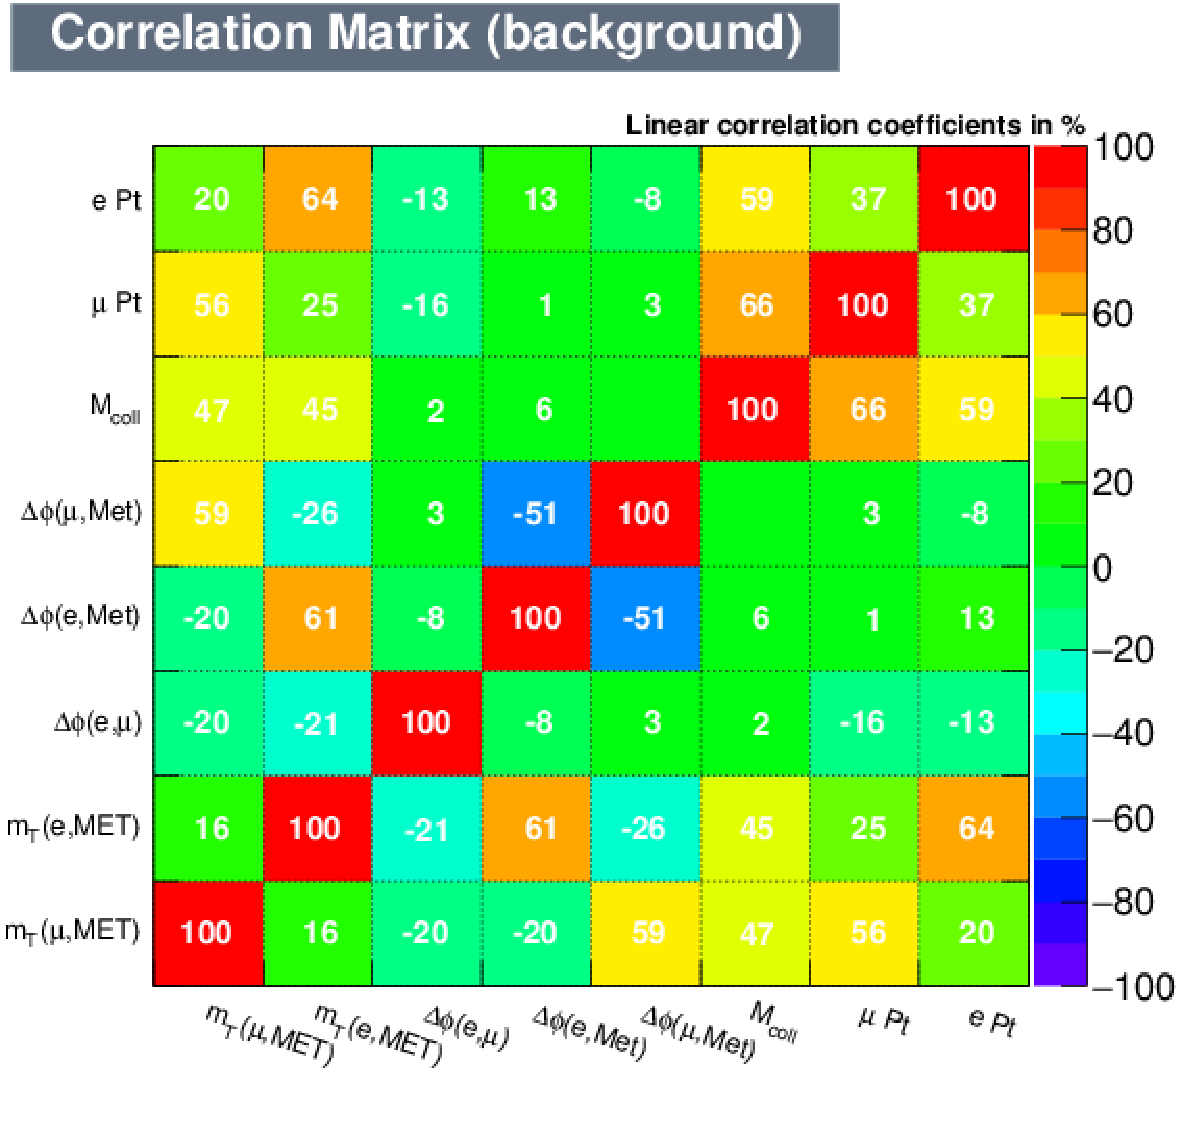
\includegraphics[width=0.48\textwidth]{plots_and_figures/chapter5/CorrelationMatrixB.pdf}
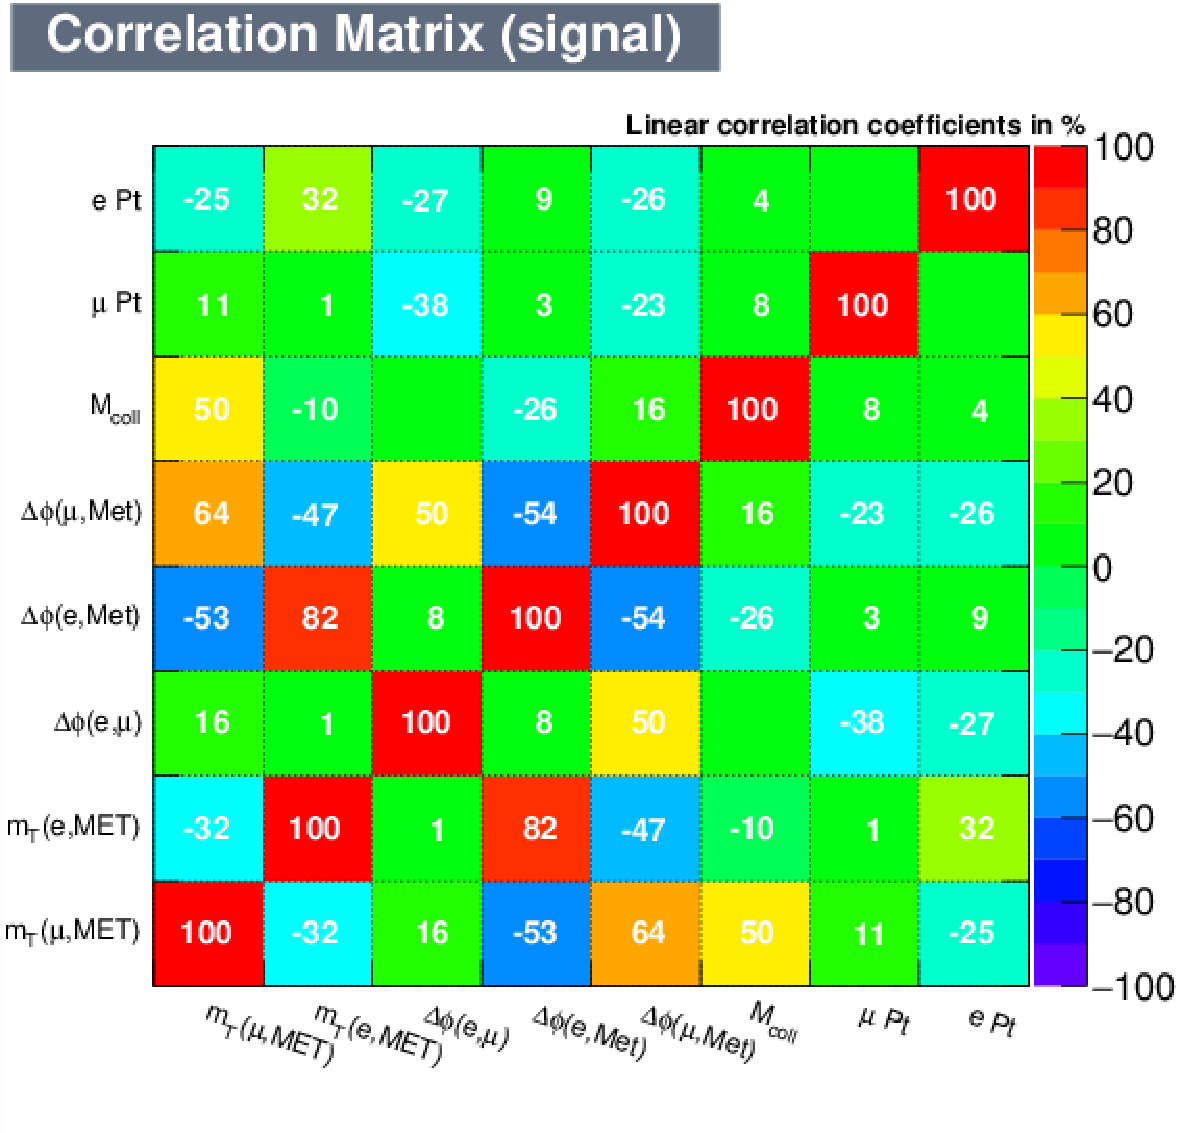
\includegraphics[width=0.48\textwidth]{plots_and_figures/chapter5/CorrelationMatrixS.pdf}\\
\end{center}
\caption{ Correlations between input variables for signal events (right) and background events (left).}
\label{fig:bdt_corr_mat}
\end{figure*}

The training was done with a 850 decision tree ensemble, each tree having a maximum depth of 4. The gini-index criterion was used for splitting the data at each node. Further, AdaBoost (adaptive boosting) method was used for boosting. A training to testing split of 70:30 split was used. Fig.~\ref{fig:BDT_response} shows the distribution of the BDT response for training and testing samples. The training and testing distributions for both signal and background events match well, suggesting that there is no overtraining. The distribution of BDT response is used in max-likelihood fit to extract results, as discussed in section~\ref{sig_ext}.  

\begin{figure*}[htpb]
\begin{center}
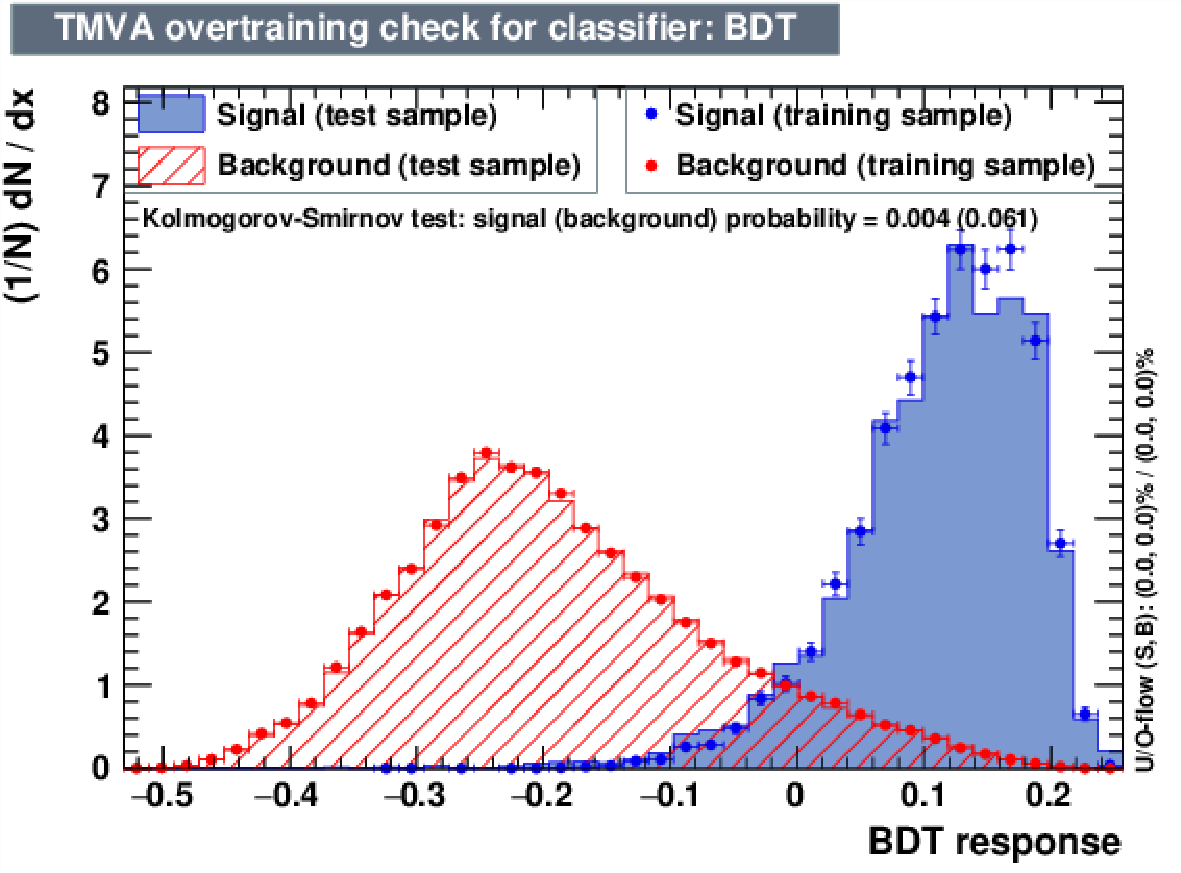
\includegraphics[width=0.48\textwidth]{plots_and_figures/chapter5/overtrain_BDT.pdf}
\end{center}
\caption{Distribution of BDT response for training (dots) and test(fill) distributions for both signal(blue) and background(red) events.}
\label{fig:BDT_response}
\end{figure*}

\section{ Heavy higgs: \Hmue analysis}
\subsection{\Hmue: Final state signature and backgrounds}
\label{HH_evt_sel}

The signature of the \Hmue analysis final state is very similar to that of \hmue. It also consists of a muon that comes promptly from the Higgs and has a hard $\pt$ spectrum, along with a softer electron that comes from the tau lepton, and missing transverse momentum from the tau decay. The $\pt^{\Pgm}$ spectrum is expected to be harder for higher H boson masses. The topologies being similar, the kinematic properties discussed in section~\ref{h125_signature} for \hmue analysis also apply to the \Hmue analysis. The H boson mass peaks for all the simulated samples illustrated in Fig~\ref{fig:sig_peaks}.


\begin{figure*}[htbp]
     \centering
     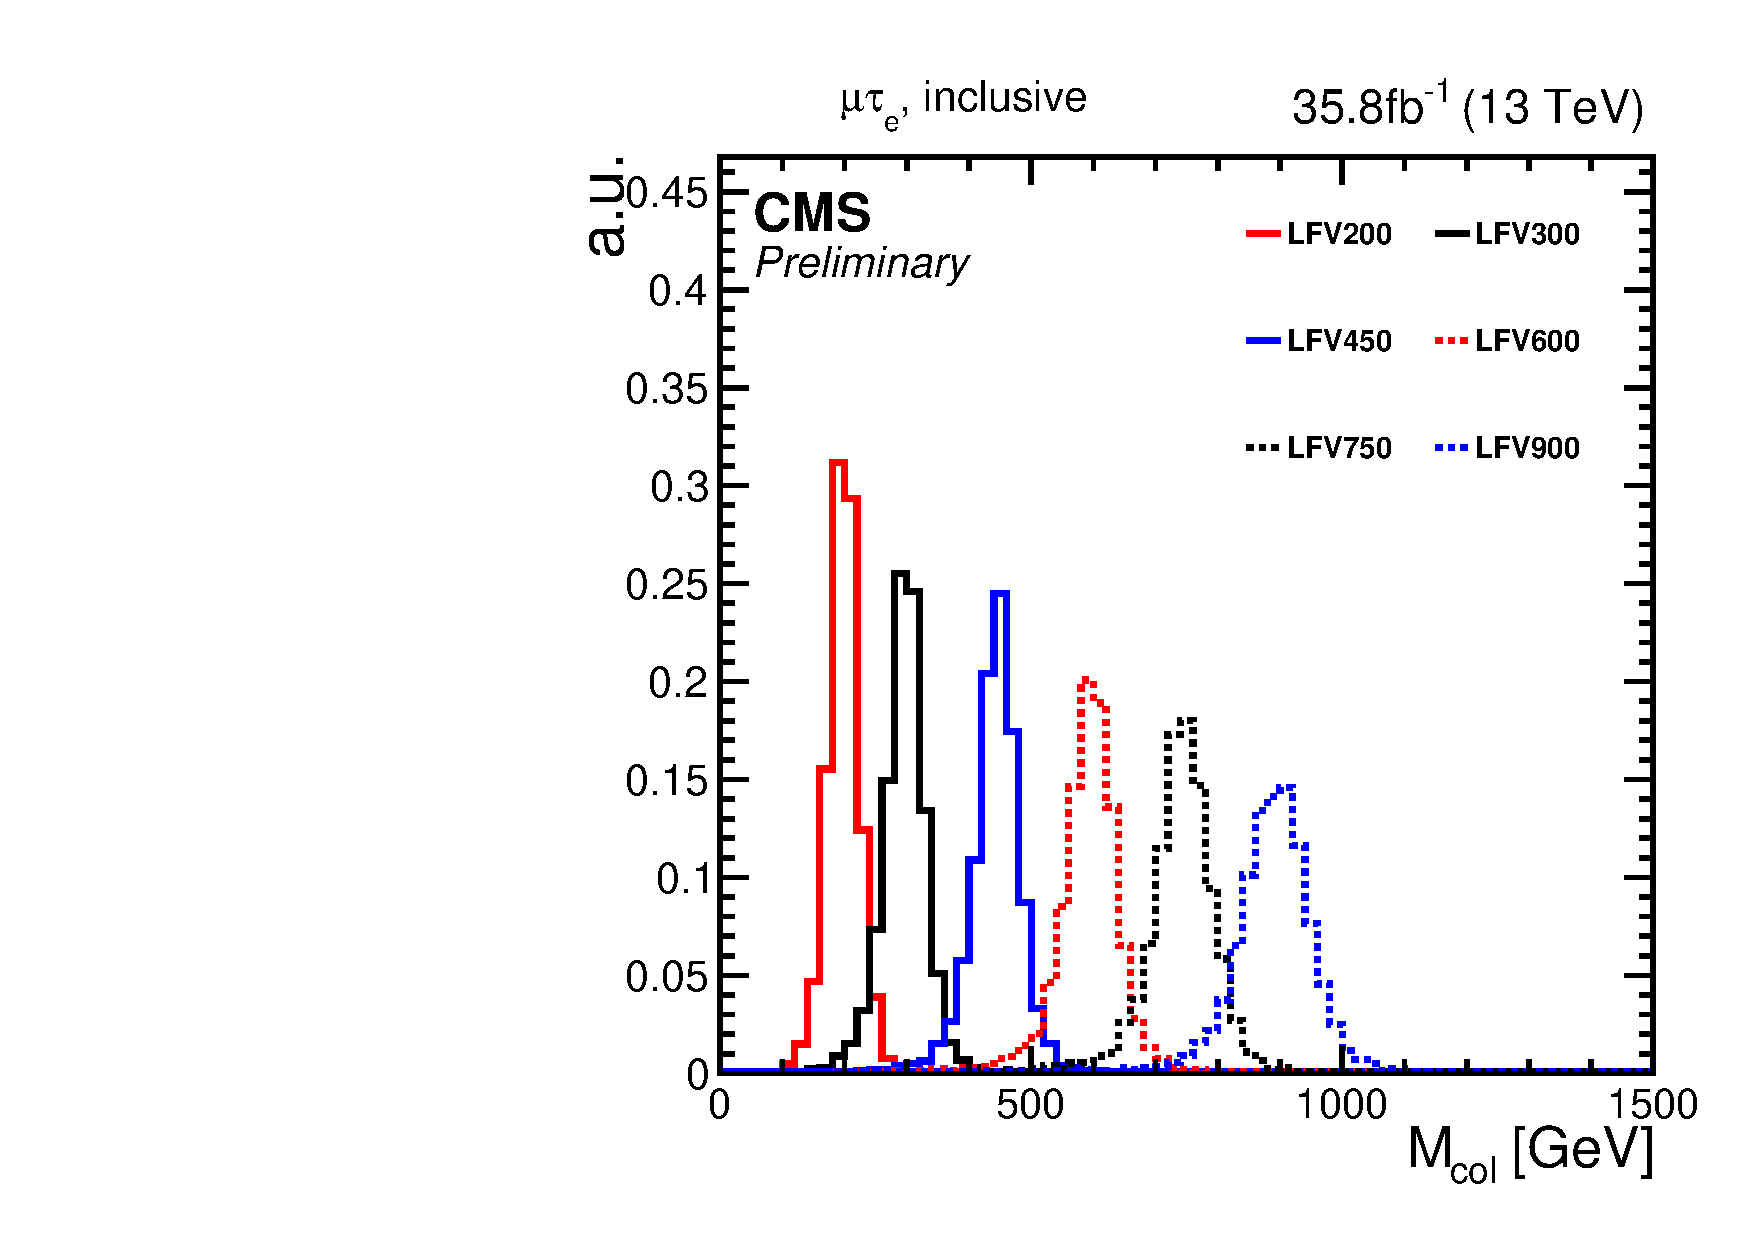
\includegraphics[width=0.5\textwidth]{plots_and_figures/chapter5/HM_signals_only_colmass.pdf}\\
     \caption{Illustration of simulated signal mass peaks for \Hmue analysis for different H boson masses.}
     \label{fig:sig_peaks}
\end{figure*}

The most dominant backgrounds for \Hmue consists of events from  \ttb and electroweak diboson production. Unlike \hmue analysis, \ztt events from Drell-Yan production form a very small background as the \ztt spectrum peaks at much lower values (around $\PZ$ boson mass) of collinear mass than the signal events coming from heavy H boson decays. The other backgrounds come from h boson decays ($h \to \Pgt\Pgt,\PW\PW$), $\PW\gamma^{(*)}+\text{jets}$ ,single top production, \wjets events, $Z\to\ell\ell$ $(\ell = \Pe, \Pgm)+\text{jets}$ and QCD multijet backgrounds. These backgrounds are described in more detail, along with their estimation and validation techniques in section~\ref{bg_val}.        

\subsection{\Hmue: Baseline selection and categorization}
\label{H_presel_cat}
The baseline selection for \Hmue is similar to that of \hmue with the exception of higher $\pt$ thresholds. Just like \hmue, an isolated and well-identified $\Pgm$ is thus required to be present along with an well-identified and isolated $\Pe$ of opposite sign charge. They are required to be separated by $\Delta R > 0.3$. The identification and isolation criteria have been described in sections~\ref{mu_recon},~\ref{e_recon} and ~\ref{isolation}. All events are required to pass a single muon trigger with the threshold of 50\GeV. The trigger selection has been described in detail in section~\ref{trigger}. The $\Pgm$ is required to have $\pt^{\Pgm} > 53$\GeV and $|\eta^{\Pgm}|<2.4$. The $\Pe$ is required to have $\pt^{\Pe} > 10$\GeV and $|\eta^{\Pe}|<2.3$. Only events with zero or one jet are considered. Jets  must have $\pt>30$\GeV, $|\eta| < 2.4 $ and satisfy the loose identification criterion described in section~\ref{jet_recon} to be considered. As only GGF production mode is considered for the \Hmue analysis, events with more than one jet make negligent contribution and are rejected. All other other criteria are same as the \hmue analysis. The entire set of baseline selection criteria for \Hmue has been summarized in table~\ref{tab:H125_base_sel}.

\begin{table}[htpb]
 \begin{center}
 \caption{Baseline selection criteria for \Hmue analysis}
  \begin{tabular}{c|c|c} \hline
    Variable    &  $\Pgm$  & $\Pe$ \\ \hline
    $\pt $       & $>53$\GeV &  $>10$\GeV                                           \\
    $|\eta| $       & $<2.4 $ &  $<2.3$                                           \\
    $I_{\text{rel}}$  & $<0.15$ &  $<0.1$                                           \\
    \multicolumn{3}{c}{Cleaning requirements} \\\hline
    \multicolumn{3}{c}{ $\Delta R(\Pgm,\Pe) > 0.3$} \\
    \multicolumn{3}{c}{No additional $\Pgm$, $\Pe$ or $\Pgt_{had}$} \\
    \multicolumn{3}{c}{No b-tagged jets with $\pt>30$\GeV} \\
    \multicolumn{3}{c}{No jets with $\Delta R(\Pgm,jet)<0.4$ and $\pt>30$\GeV} \\
    \multicolumn{3}{c}{No jets with $\Delta R(\Pe,jet)<0.4$ and $\pt>30$\GeV }\\
    \hline
  \end{tabular}
  \label{tab:H125_base_sel}
  \end{center}
\end{table}

The events are then divided into  categories, with motivations similar to the \hmue analysis (see section~\ref{h125_presel_cat}), on the basis of number of jets present in the event. The two categories for \Hmue are:
\begin{itemize}%[itemsep=5pt]
\item \textbf{0-jet category}: These are events that do not have any jet. This category enhances the gluon-gluon fusion (GGF) contribution.
\item \textbf{1-jet category}: Events that have 1 jet are put in this category. This category enhances the GGF production with initial state radiation (ISR).
\end{itemize}

The distributions of several kinematic variables after the baseline selection and categorization are shown in Figs.~\ref{fig:Hmutaue_presel1} and ~\ref{fig:Hmutaue_presel2}.

\begin{figure*}[htbp]
     \centering
     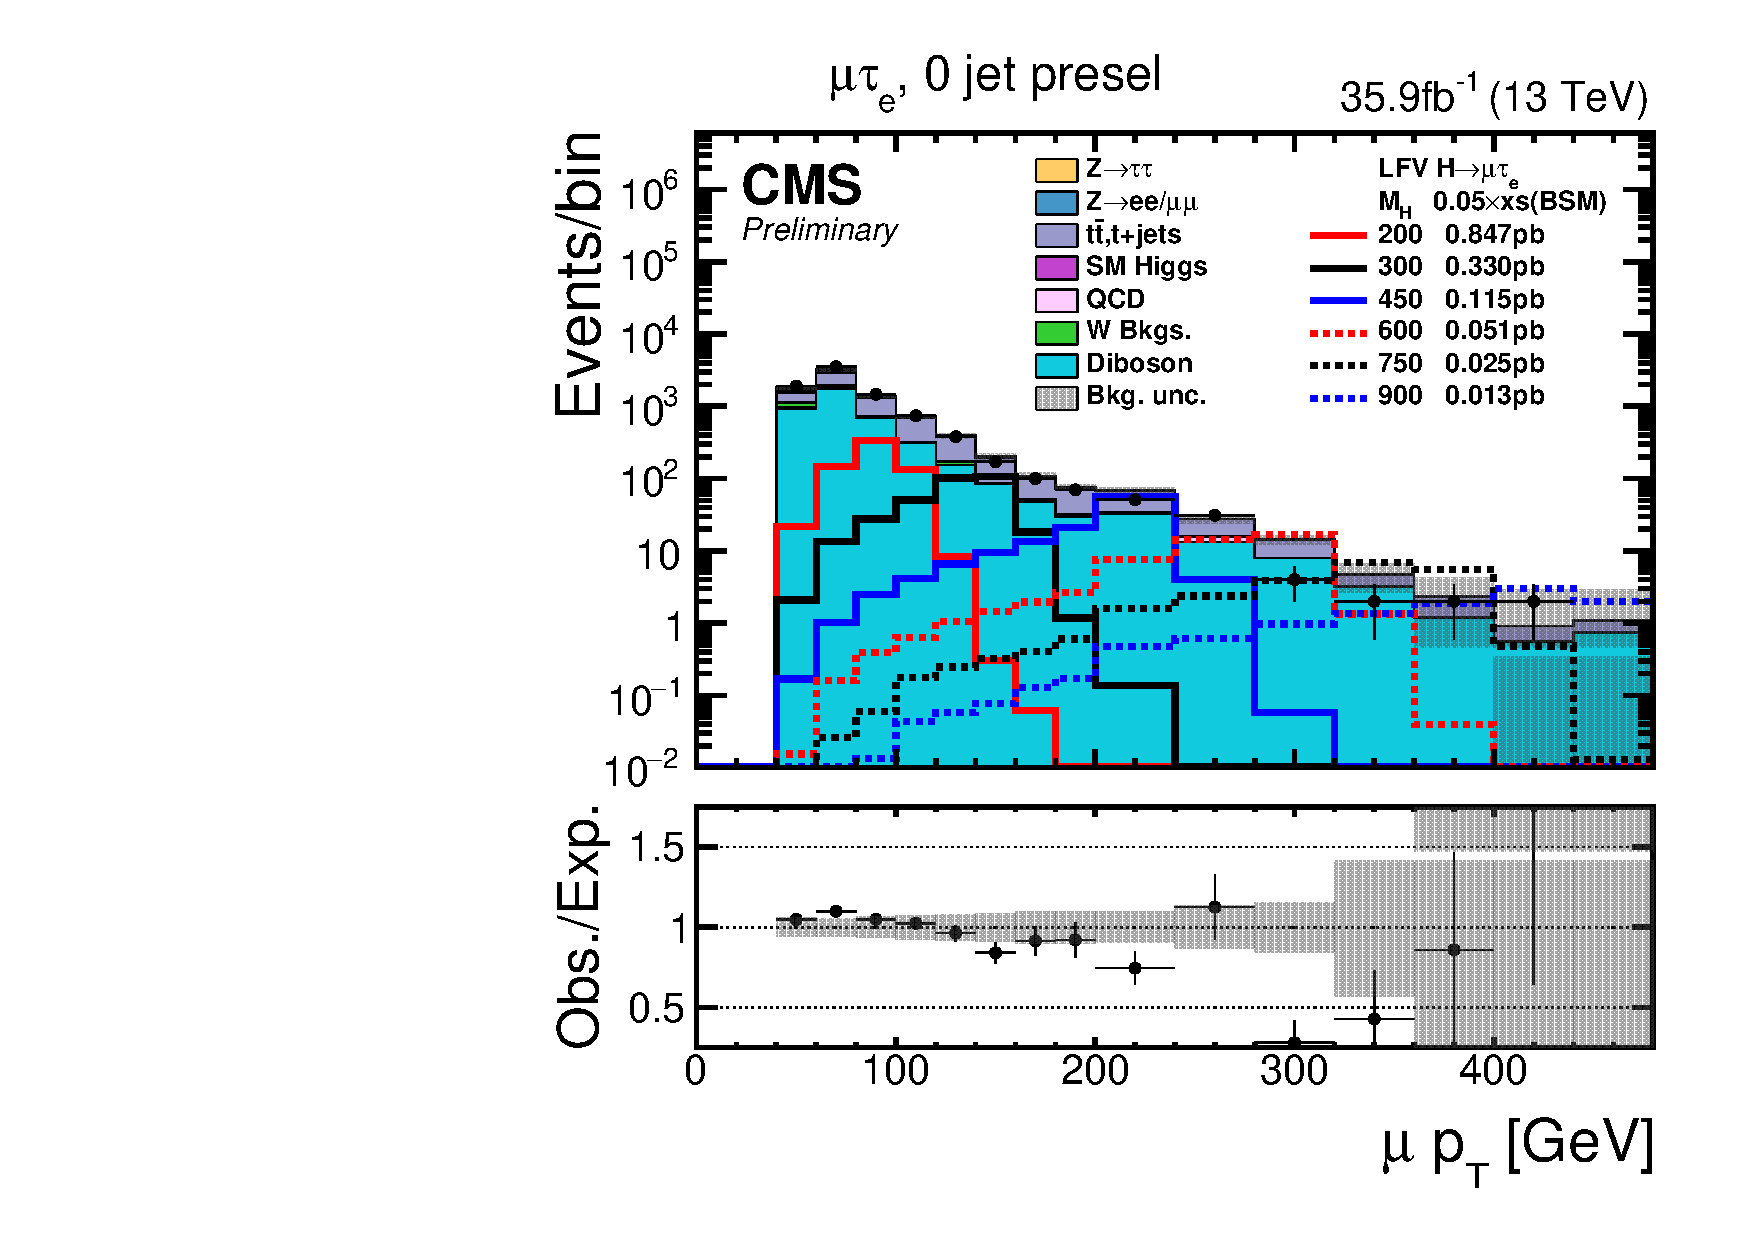
\includegraphics[width=0.48\textwidth]{plots_and_figures/chapter5/preselection_HM/log_mutaue_0jet_presel_mPt.pdf}
     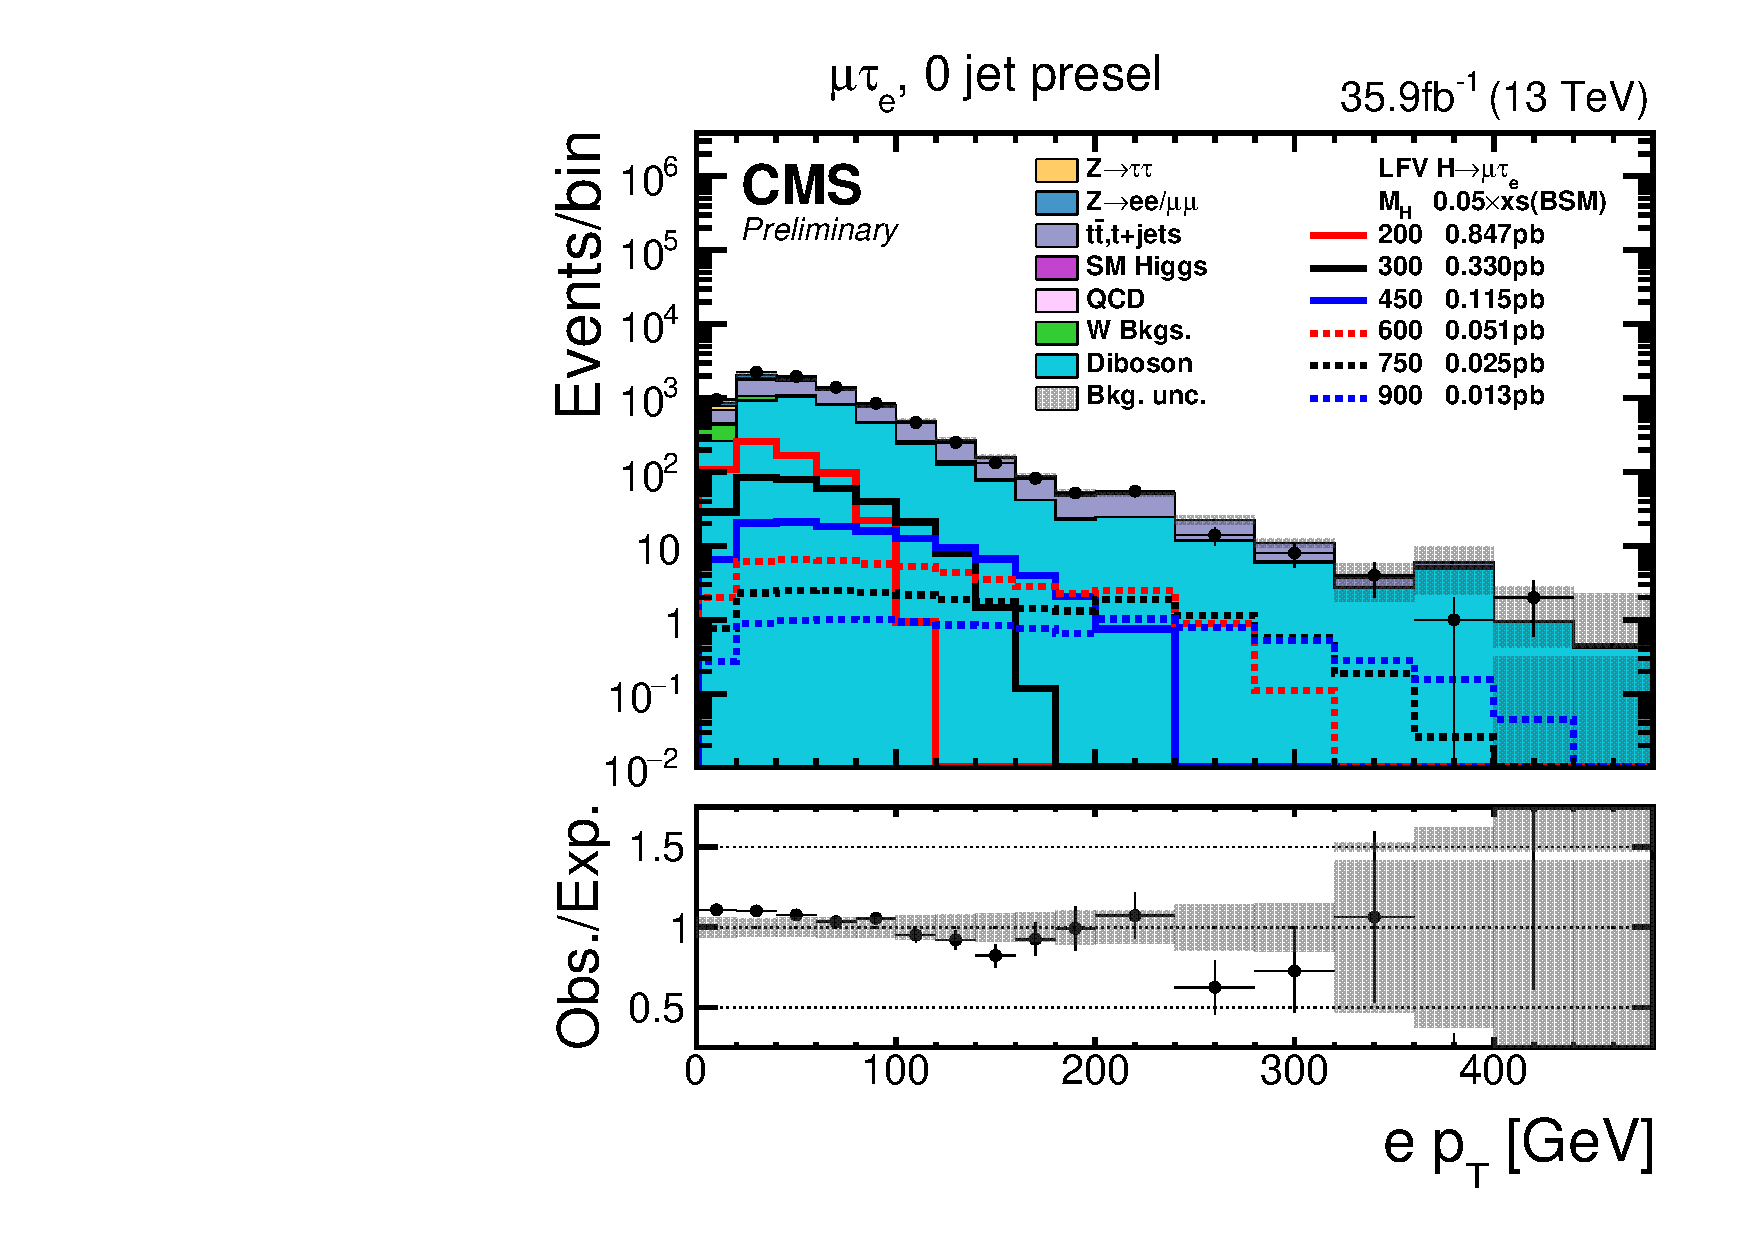
\includegraphics[width=0.48\textwidth]{plots_and_figures/chapter5/preselection_HM/log_mutaue_0jet_presel_ePt.pdf}\\
     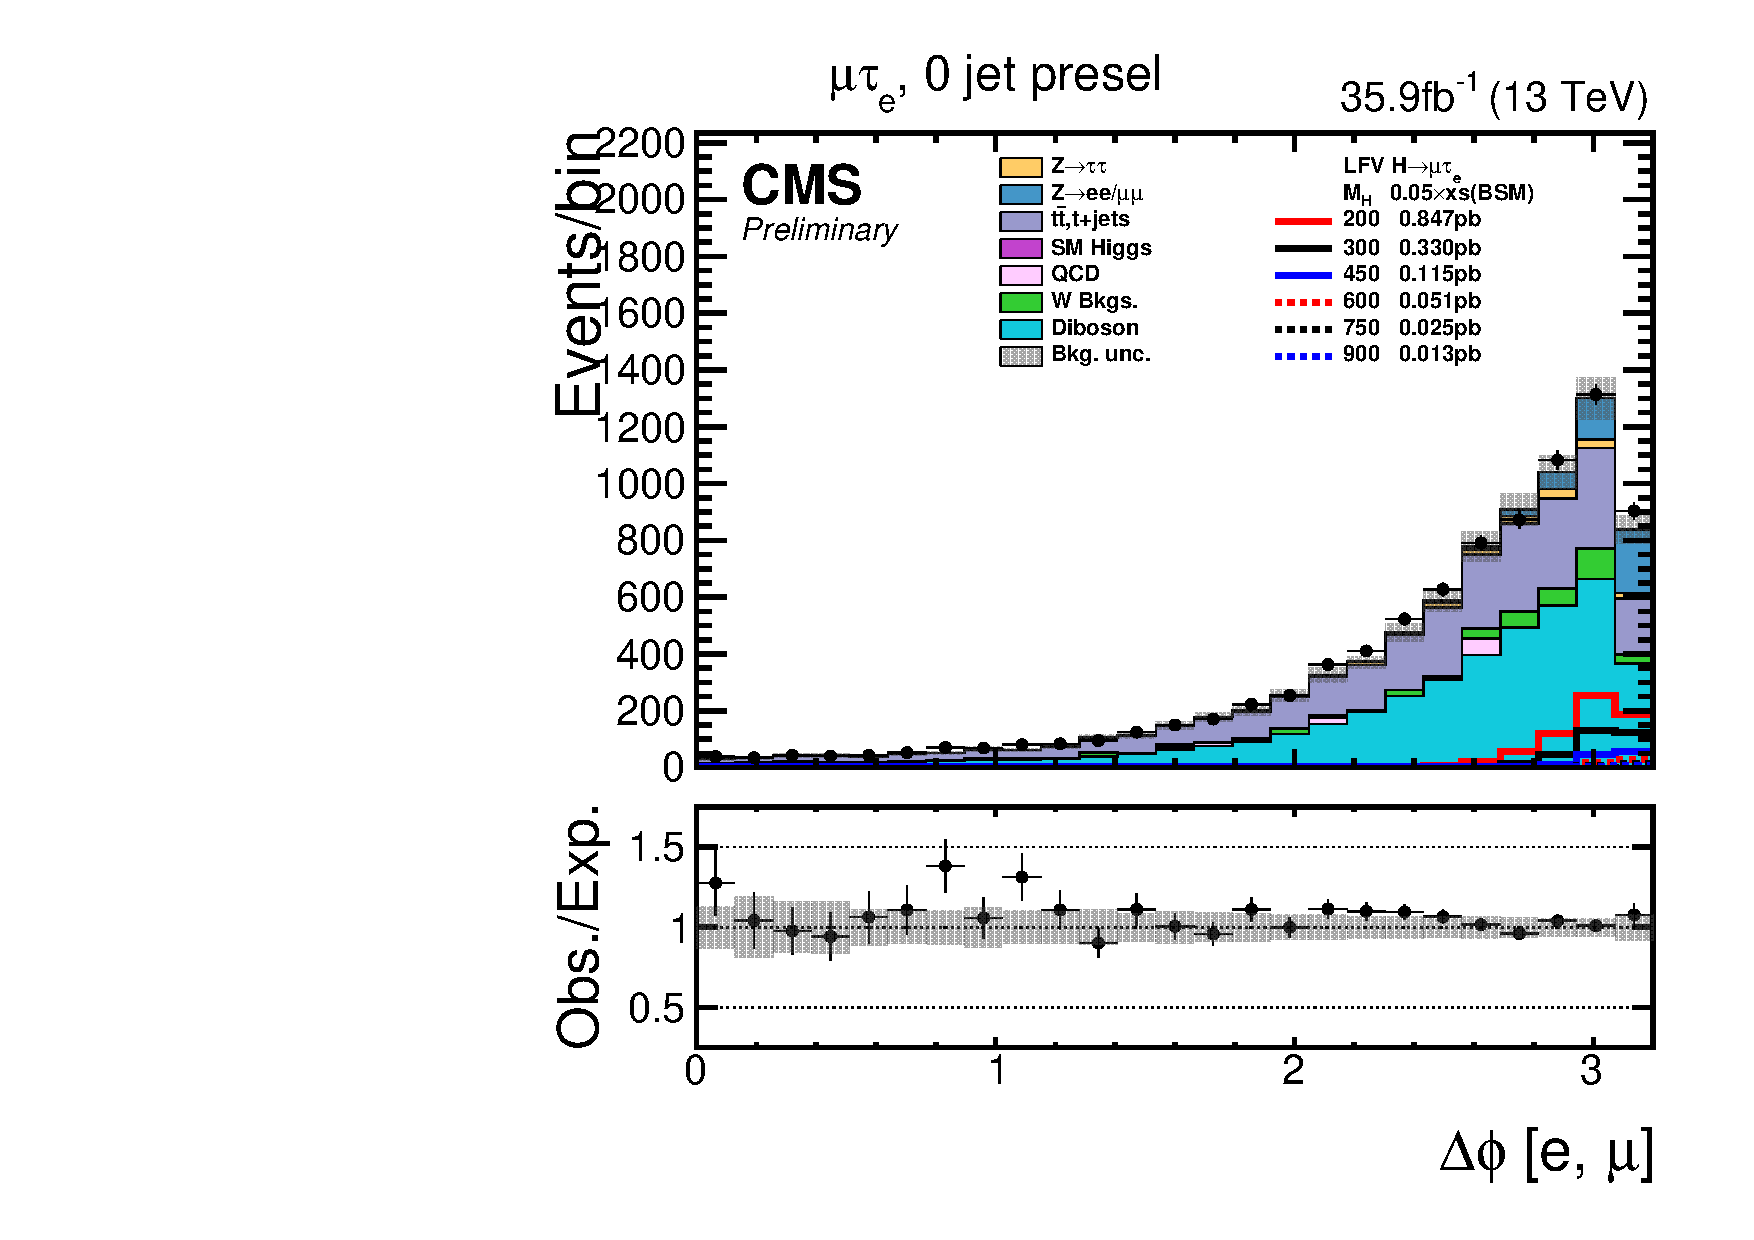
\includegraphics[width=0.48\textwidth]{plots_and_figures/chapter5/preselection_HM/mutaue_0jet_presel_dphiemu.pdf}
     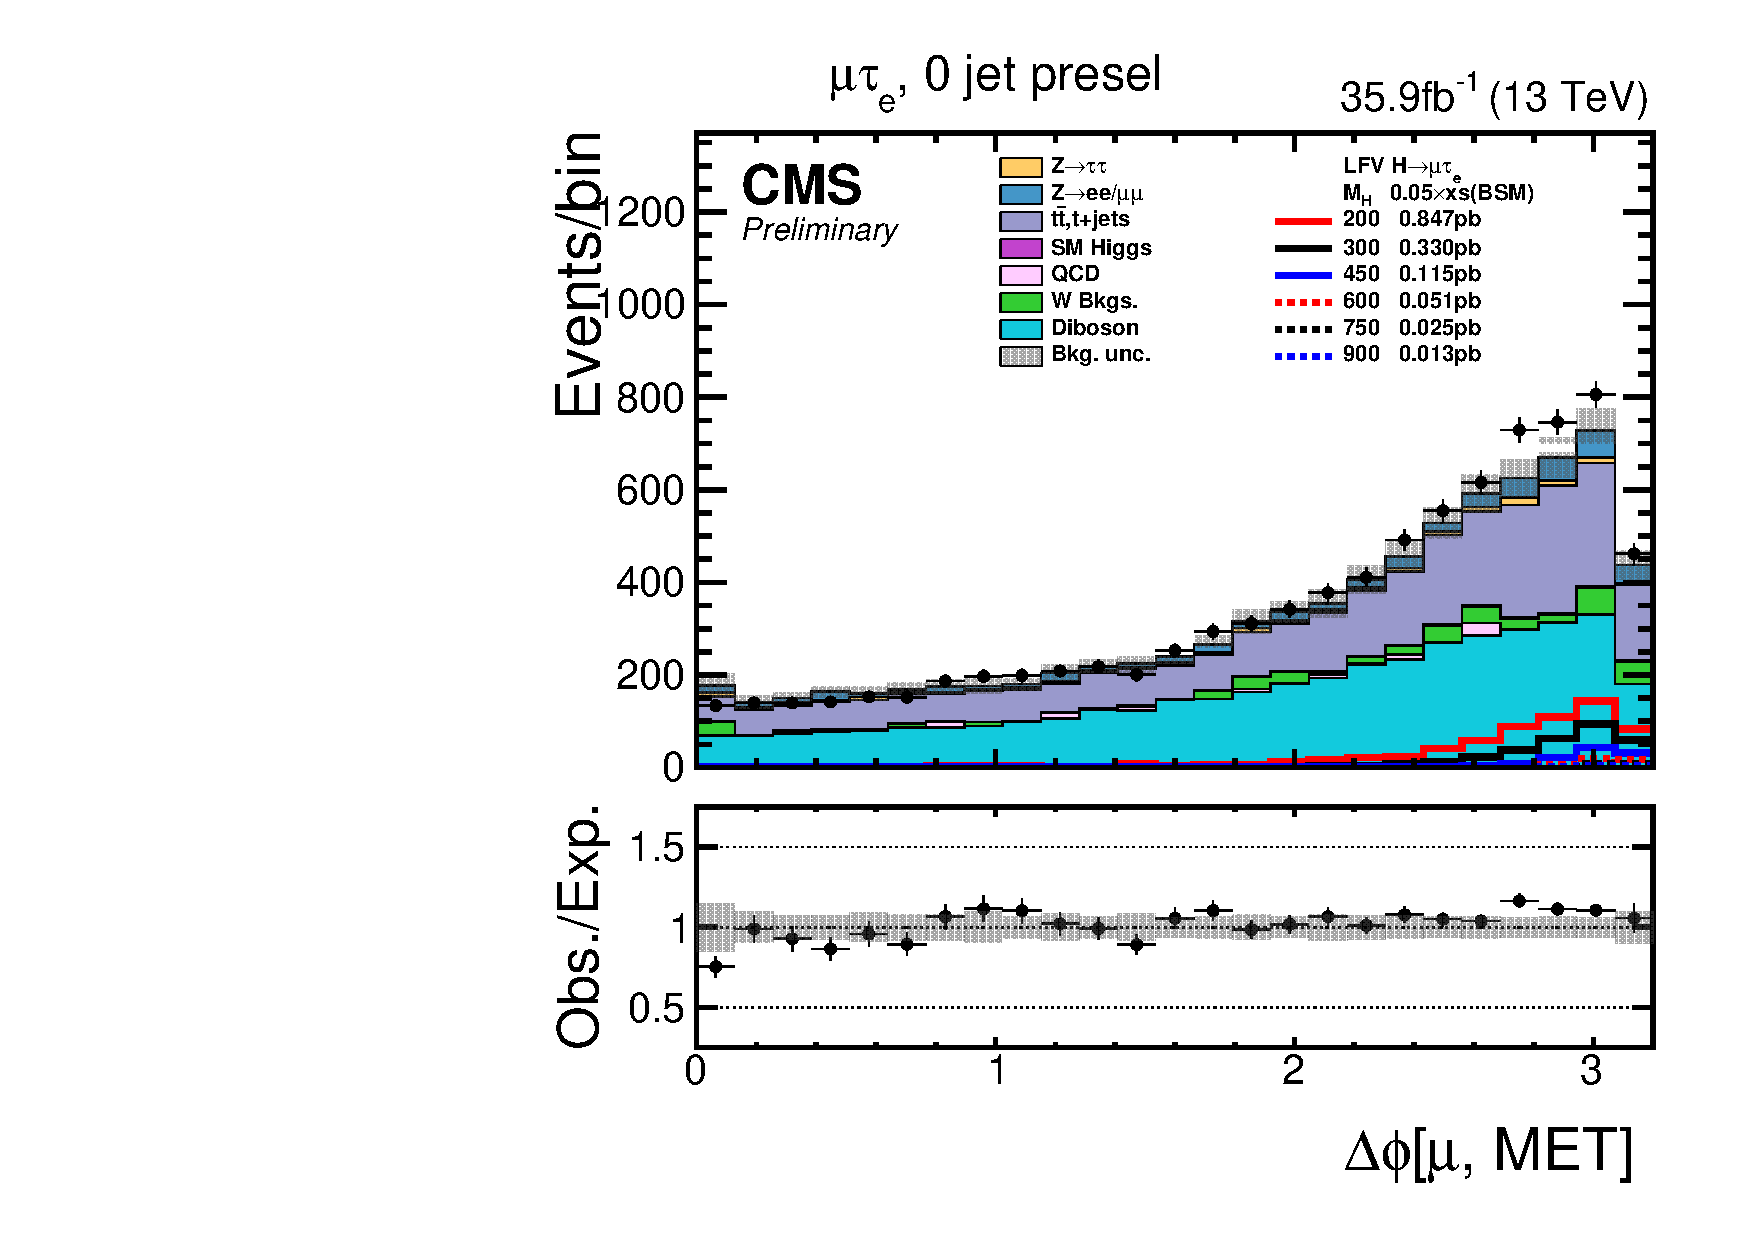
\includegraphics[width=0.48\textwidth]{plots_and_figures/chapter5/preselection_HM/mutaue_0jet_presel_dphiMuMet.pdf}\\
     \caption{Distributions of kinematic variables after baseline selction for 0-jet category of \Hmue analysis.}
     \label{fig:Hmutaue_presel1}
\end{figure*}

\begin{figure*}[htbp]
     \centering
     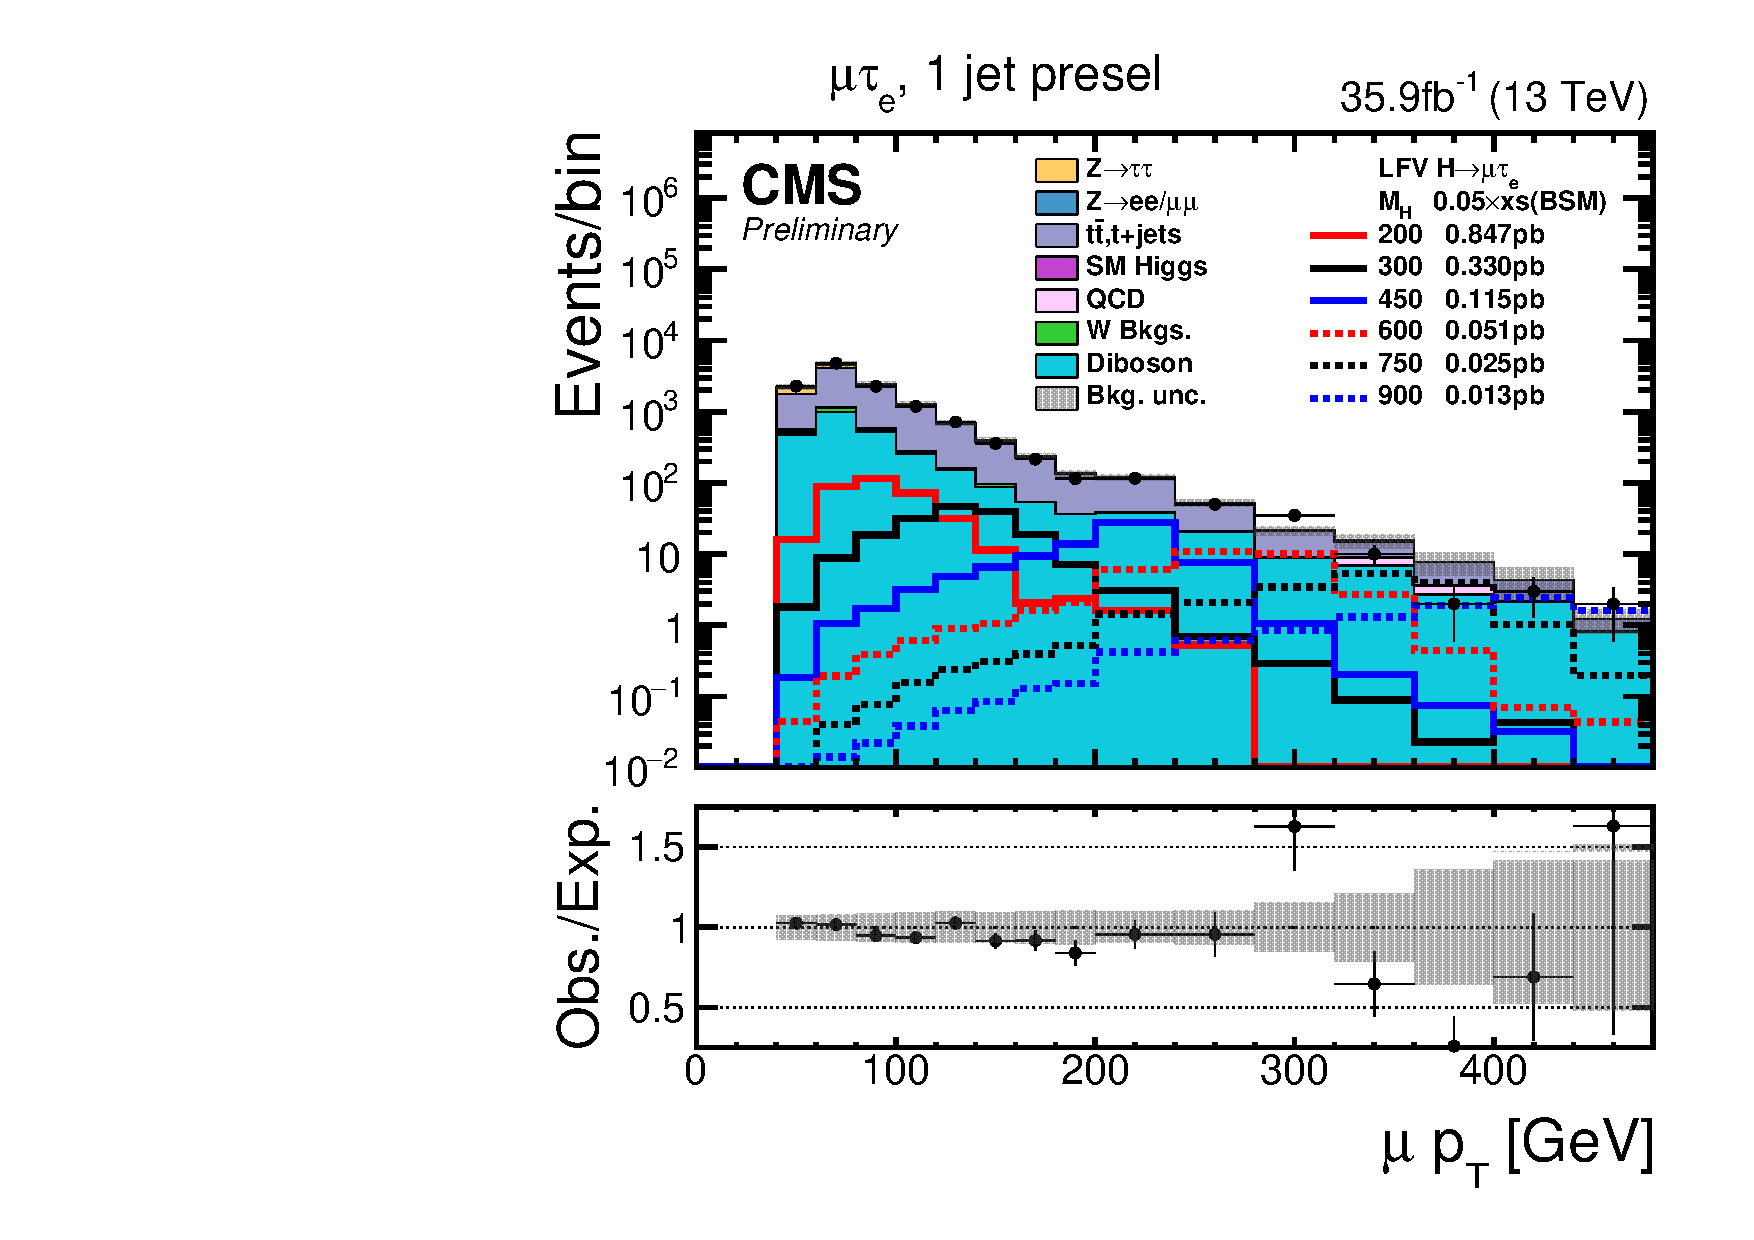
\includegraphics[width=0.48\textwidth]{plots_and_figures/chapter5/preselection_HM/log_mutaue_1jet_presel_mPt.pdf}
     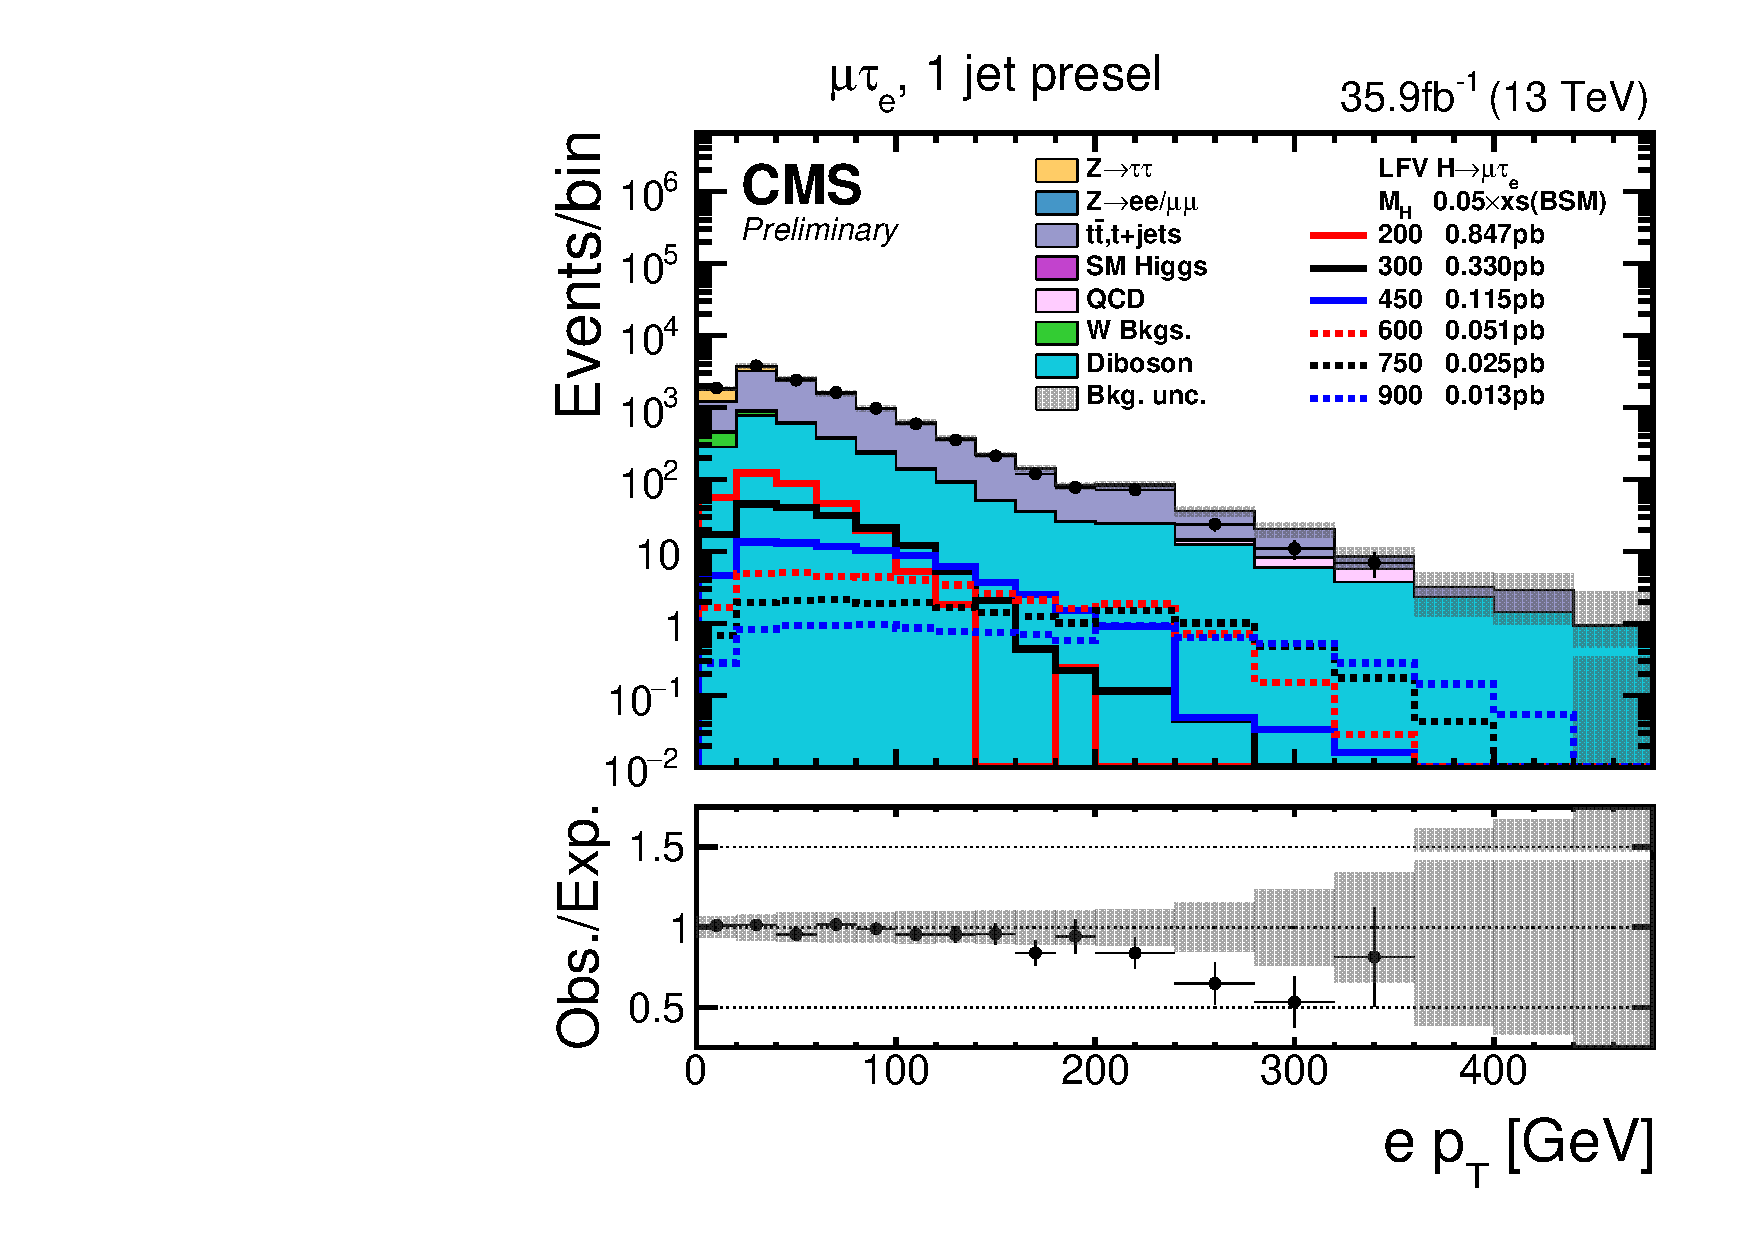
\includegraphics[width=0.48\textwidth]{plots_and_figures/chapter5/preselection_HM/log_mutaue_1jet_presel_ePt.pdf}\\
     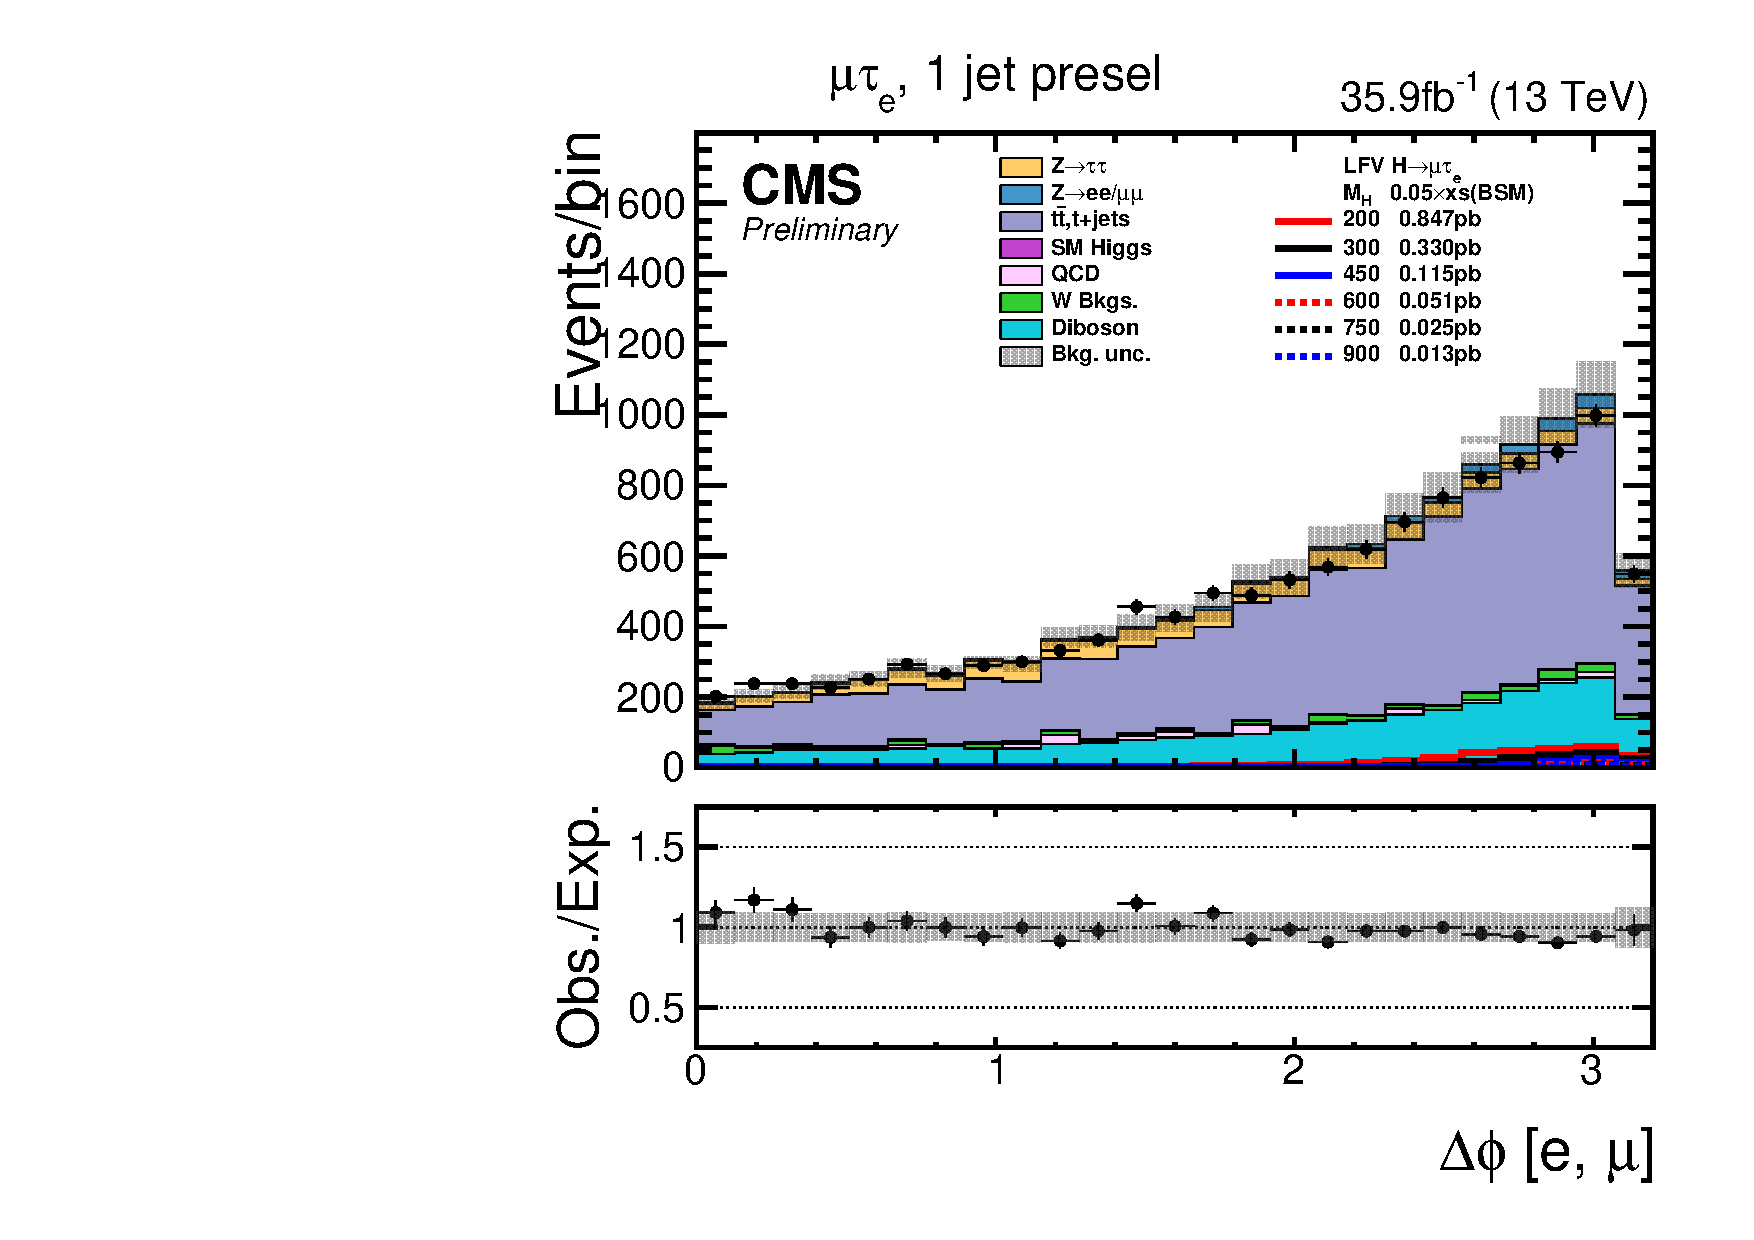
\includegraphics[width=0.48\textwidth]{plots_and_figures/chapter5/preselection_HM/mutaue_1jet_presel_dphiemu.pdf}
     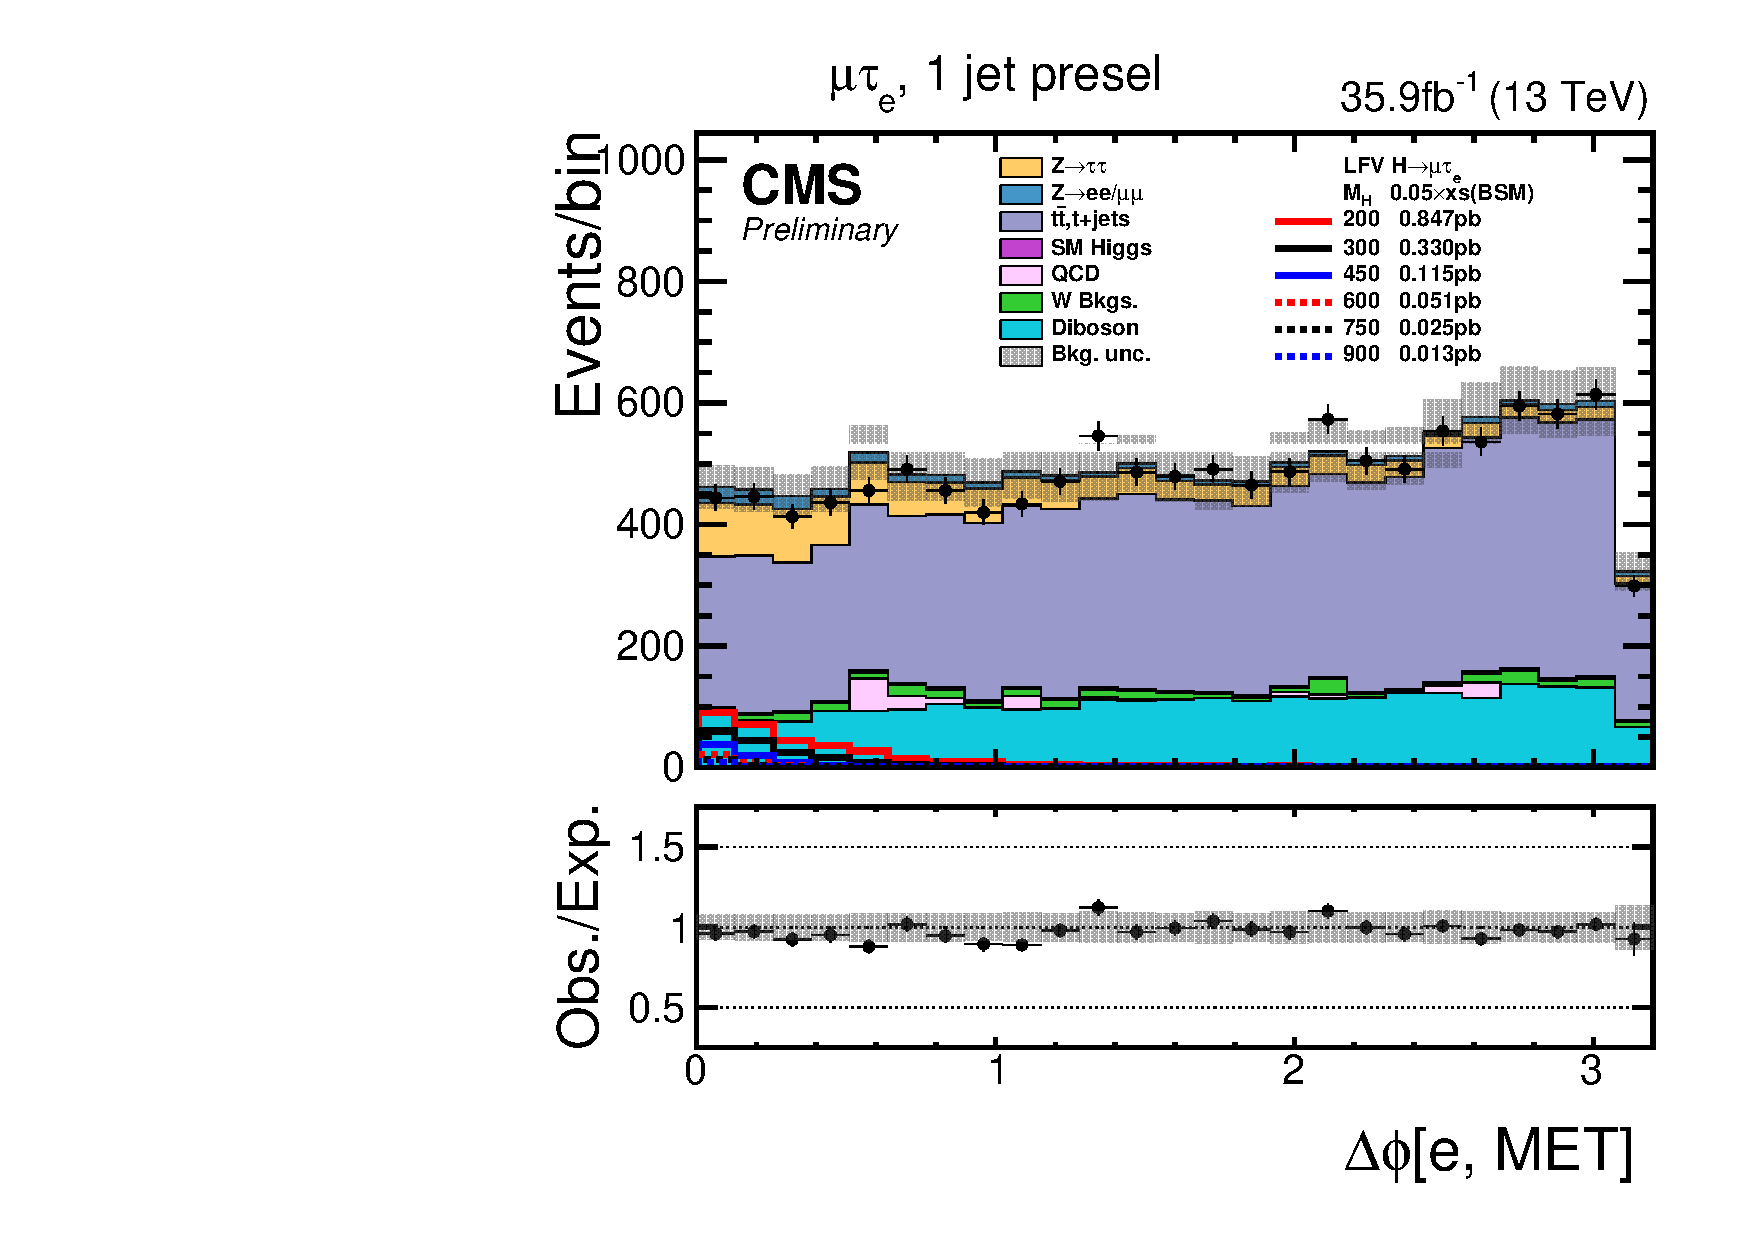
\includegraphics[width=0.48\textwidth]{plots_and_figures/chapter5/preselection_HM/mutaue_1jet_presel_dphiEMet.pdf}\\
     \caption{Distributions of kinematic variables after baseline selction for 1-jet category of \Hmue analysis.}
     \label{fig:Hmutaue_presel2}
\end{figure*}


\subsection{\Hmue: \mcol fit selection}
\label{H125_cb_sel}
 Just like the \mcol fit method in \hmue, the selection is performed by placing kinematic cuts on several variables to enhance the signal-to-background ratio. The variables considered are: $\dphiemu$, $\dphiemet$, $\dphimumet$, $M_T(\Pgm)$ and $M_T(\Pe)$. In addition, the $\pt$ of the $\Pgm$ and $\Pe$ are also considered. Since we are looking for a decay in an extended mass range (200-900 GeV) in \Hmue, and not in a particular region like the \hmue analysis, the potential effect of background  mimicking the signal, in particular due to higher $\pt$ thresholds of the leptons, is not apparent. The motivations for using these variables remain much the same like the \hmue analysis owing to similarities in topology. They are motivated by the facts that the only source of MET is the $\Pgt$, and the  $\Pgt$ being lighter than the H, its visible products are closely aligned, and the $\pt$ spectrum of the prompt lepton ($\Pgm$) is hard.

The procedure for optimization of the thresholds of for these variables is exactly the same as described in section~\ref{h125_cb_sel}. Further to get better sensitivity in the entire mass range from 200 to 900 GeV, two separate sets of thresholds are optimized, for each category. One set is optimized to provide better sensitivity in the 200-450 GeV mass range. The simulated signal for the H mass of 200 GeV is used when calculating expected limits during the optimization procedure for this mass range. The other set is optimized to provide better sensitivity in 450-900 GeV mass range. The simulated signal for H mass of 450 GeV is used when calculating expected limits during the optimization procedure for this mass range. A few illustrations of the optimization procedure are shown in Fig.~\ref{fig:Hmue_limit_opt}. The final set of thresholds arrived at in this manner, for both mass ranges and both categories of the \Hmue \mcol fit analysis, are listed in Table.~\ref{tab:H125_sel_cuts}. The \mcol distributions after requiring these selections is used in a max-likelihood fit to extract results, as discussed in section~\ref{sig_ext}.


 \begin{figure}[htbp]
     \centering
     \subfigure[Low mass range 0 jet $\Delta\phi(\Pe, \ptvecmiss)$]{ 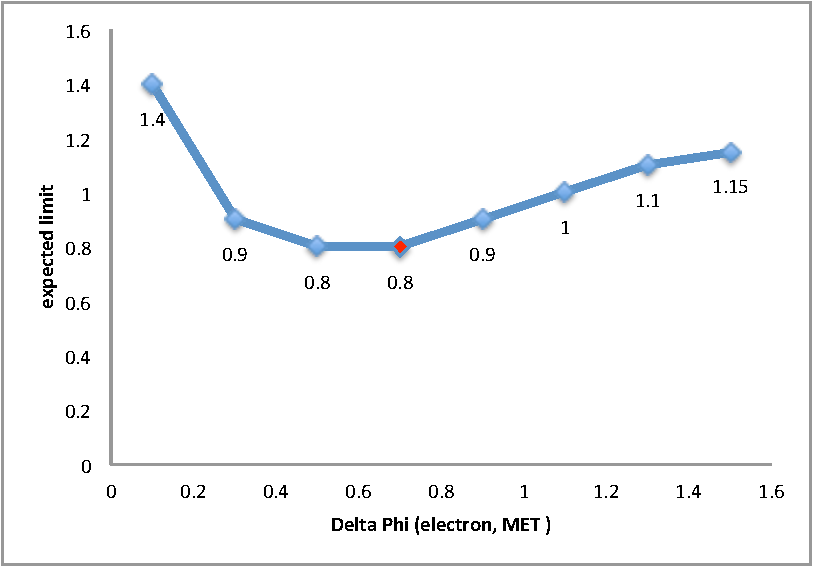
\includegraphics[width=0.375\textwidth]{plots_and_figures/chapter5/limit_opt/200_0jet_dphiemet.pdf}}
     \subfigure[Low mass range 1 jet $\Delta\phi(\Pe, \ptvecmiss)$]{ 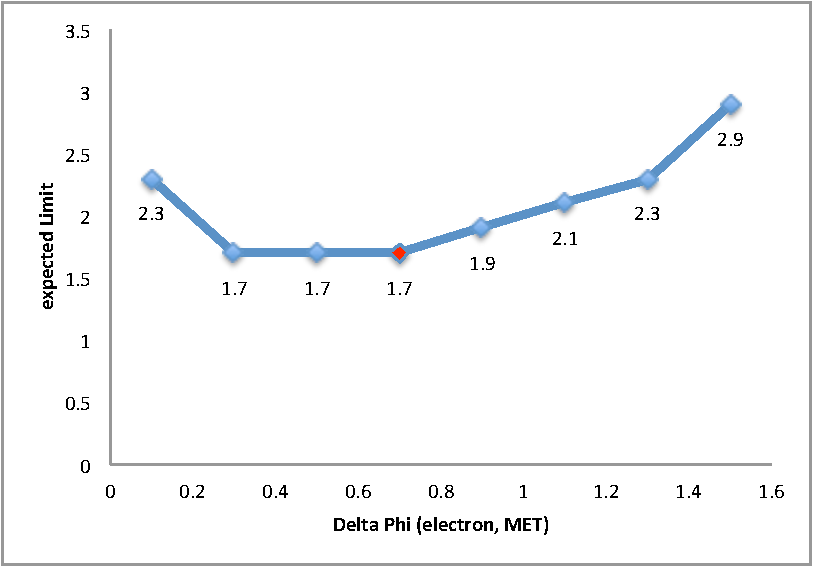
\includegraphics[width=0.375\textwidth]{plots_and_figures/chapter5/limit_opt/200_1jet_dphiemet.pdf}}\\
     \subfigure[Low mass range 0 jet $\Delta\phi(\Pe, \Pgm)$]{ 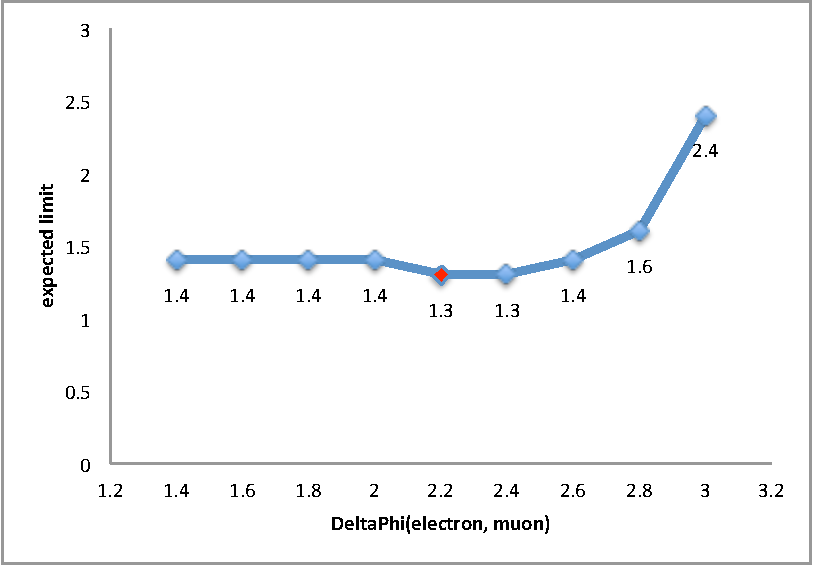
\includegraphics[width=0.375\textwidth]{plots_and_figures/chapter5/limit_opt/200_0jet_dphiemu.pdf}}
     \subfigure[Low mass range 0 jet $\pt^{\Pe}$]{ 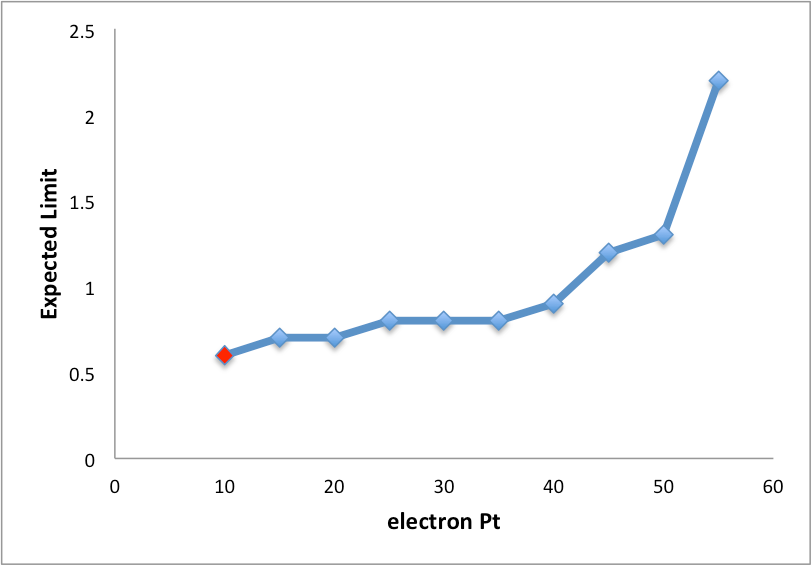
\includegraphics[width=0.375\textwidth]{plots_and_figures/chapter5/limit_opt/200_0jet_ept.pdf}}\\
     \subfigure[High mass range 1 jet $\pt^{\Pgm}$]{ 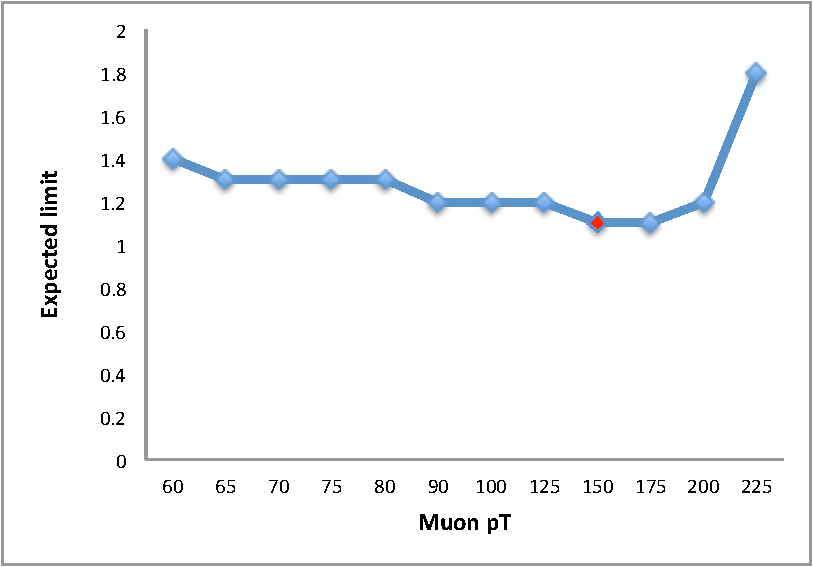
\includegraphics[width=0.375\textwidth]{plots_and_figures/chapter5/limit_opt/450_1jet_mupt.pdf}}
     \subfigure[High mass range 0 jet $\Delta\phi(\Pe, \ptvecmiss)$]{ 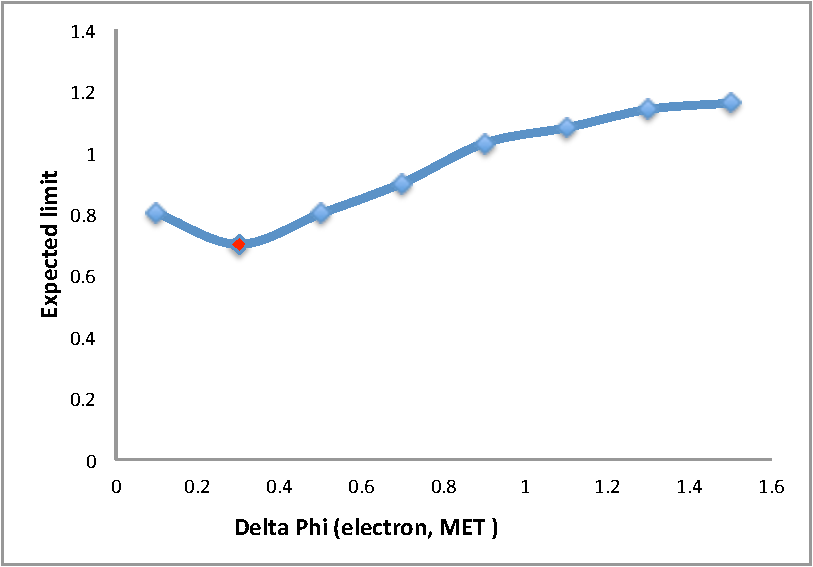
\includegraphics[width=0.375\textwidth]{plots_and_figures/chapter5/limit_opt/450_0jet_dphiemet.pdf}}\\
     \subfigure[High mass range 1 jet $\Delta\phi(\Pe, \ptvecmiss)$]{ 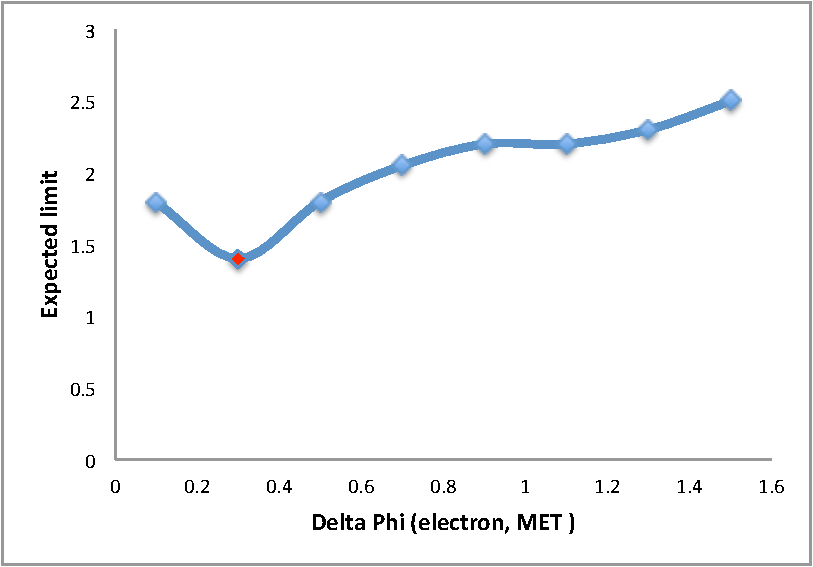
\includegraphics[width=0.375\textwidth]{plots_and_figures/chapter5/limit_opt/450_1jet_dphiemet.pdf}}
     \subfigure[High mass range 1 jet $\pt^{\Pe}$]{ 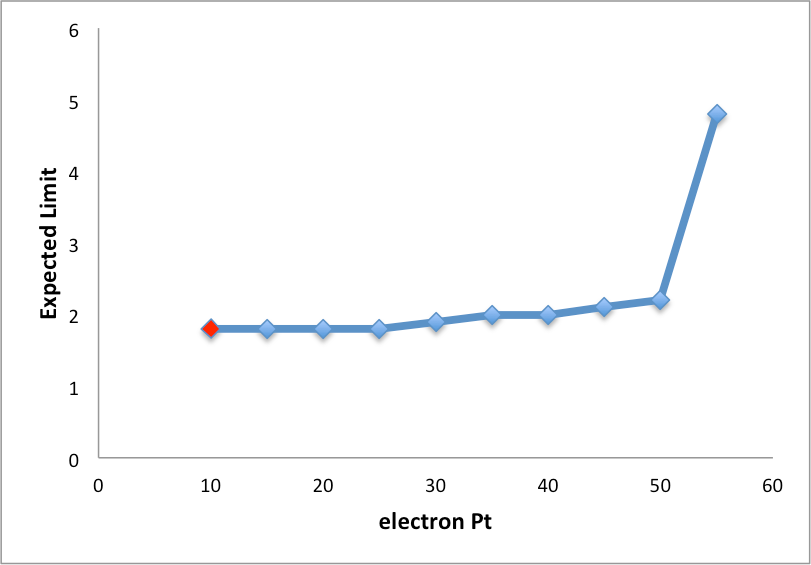
\includegraphics[width=0.375\textwidth]{plots_and_figures/chapter5/limit_opt/450_1jet_ept.pdf}}\\
     \caption{Examples of cut optimisation for the $\Hmue$ analysis.}
     \label{fig:Hmue_limit_opt}
\end{figure}

 \begin{table}[hbtp]
  \begin{center}
  \caption{Final selection criteria in each category  of the $\Hmue$ analysis}
  \begin{tabular}{c|cc}
  \hline
  & Low mass range & High mass range\\ \hline
  \multirow{3}{*}{0-jet}
  & $\pt^{\Pgm}>60$\GeV, $\pt^{\Pe}>10$\GeV &  $\pt^{\Pgm}>150$\GeV, $\pt^{\Pe}>10$\GeV\\
  & $\Delta\phi(\Pe, \ptvecmiss)<0.7$ & $\Delta\phi(\Pe, \ptvecmiss)<0.3$ \\
  & $\Delta\phi(\Pe, \Pgm)>2.2$ & $\Delta\phi(\Pe, \Pgm)>2.2$ \\
    [\cmsTabSkip]\\
    [\cmsTabSkip]
  \multirow{3}{*}{1-jet}
  & $\pt^{\Pgm}>60$\GeV, $\pt^{\Pe}>10$\GeV & $\pt^{\Pgm}>150$\GeV, $\pt^{\Pe}>10$\GeV\\
  & $\Delta\phi(\Pe, \ptvecmiss)<0.7$ & $\Delta\phi(\Pe, \ptvecmiss)<0.3$\\
  & $\Delta\phi(\Pe, \Pgm)>2.2$& $\Delta\phi(\Pe, \Pgm)>2.2$\\
  \hline
  \end{tabular}
   \label{tab:H125_sel_cuts}
\end{center}
\end{table}







% % uncomment the following lines,
% if using chapter-wise bibliography
%
% \bibliographystyle{ndnatbib}
% \bibliography{example}




%
%
% Chapter 6
%

\chapter{Search for LFV decays of h125}

This chapter describes the analysis in search for lepton flavor violating decay of the h125 boson into a muon and an electronically decaying tau lepton. The motivation for this search is discussed in the introduction and theory sections. In the following sections the dataset and MC samples used, event selection and subsequent analysis strategy, systematic uncertainties affecting the analysis and finally the results are described in detail.




% % uncomment the following lines,
% if using chapter-wise bibliography
%
% \bibliographystyle{ndnatbib}
% \bibliography{example}




%
%
% Chapter 7
o%

\chapter{Signal extraction and systematic uncertainties}
\label{sig_ext}
\section{Introduction}
The analysis is, in its essence, a sophisticated counting experiment. The presence of a signal is indicated by an excess of events over the predicted background, in the distribution of a signal variable. For our analyses the signal variables are collinear mass or BDT output, as described in Sections~\ref{evt_sel} and ~\ref{chap:event_sim}. Given that there are several uncertainties, both experimental and theoretical and also due to the innate randomness in the process, it is possible that an excess is observed when there is no signal. So, when an excess is observed, a p-value which represents the probability that the excess is due to statistical fluctuations is computed. A very low p-value is taken to indicate that the excess corresponds to an observed signal and not merely a statistical fluctuation. Conversely, if no excess is observed (upper exclusion) limits are set on the product of branching fraction and production cross-section. A 95\% CL (confidence level) is taken as a requirement for ruling out a signal at or above a certain value known i.e. upper exclusion limit. The first part of this chapter describes the statistical methods used, that very closely follow the procedure used for LHC Higgs boson search and described in ~\cite{note2011}.

Several sources of systematic uncertainties need to be considered when making the above measurement. The sources of these uncertainties can be theoretical, experimental or purely statistical in nature. Further, they can effect only the overall scale of the distributions (used to make the measurement), or effect there shape i.e. change the scale differently in each bin of the distribution. All the uncertainties used in the analyses and their sources are described in the second part of this chapter.      



\section{Statistical methods for signal extraction}
In the following section, the expected signal event yields are denoted by $s$, and backgrounds by $b$. The parameter $\mu$ that appears is the signal strength modifier, which changes the signal production cross-sections of all the production mechansims by exactly the same scale $\mu$.
\label{stat_meth}
\subsection{Likelihood function}
The Poisson distribution is an appropriate model for n, the number of times an event occurs in an interval if the following assumptions are true~\cite{poisson_wiki}.
\begin{itemize}
\item The occurrence of one event does not affect the probability that a second event will occur. That is, events occur independently.
\item The rate at which events occur is constant. The rate cannot be higher in some intervals and lower in other intervals. This rate is the average number of events in the interval. $\lambda$.
\item Two events cannot occur at exactly the same instant; instead, at each very small sub-interval exactly one event either occurs or does not occur.
\end{itemize}
The poisson probablity of distribution is then given by:
\begin{equation}
  P(n_events)=\frac{e^{-\lambda}\lambda^{n}}{n!}
\end{equation}
For a counting experiments such as ours, the above conditions approximately hold. The expected number of events is $\mu\cdot s + b$. The likelihood function $\mathcal{L}(data|\mu)$ is then given by:
\begin{equation}
  \mathcal{L}(data|\mu)=\prod_{i=1}^{bins}\frac{(\mu\cdot s_i + b_i)^{n_i}}{n_{i}!}e^{-\mu\cdot s_i - b_i}
\end{equation}
,where $n_i$ is the number of events observed in the bin i of the distribution, and $s_i$ and $b_i$ are expected number of signal and background events in that bin respectively.


\subsection{Treatment of systematic uncertainties}
\label{sys_treat}
All systematic uncertainties are handled by introducing them as nuisance parameters. Nuisance parameters are parameters that influence the model but are not of interest in our measurement, e.g., if we are interested in knowing only the mean of a population that is expected to be distributed as a gaussian, the standard deviation becomes a nuisance parameter for the model that we fit. In our experiment, the nuisance parameters are embedded into the likelihood function. In order for the likelihood function to have a clean factorised form ~\cite{note2011}, all sources of uncertainties considered are considered 100\%-corrrelated or uncorrelated. If an uncertainty is partially correlated, it is either separated into 100\%-corrrelated or uncorrelated components, or considered 100\%-corrrelated or uncorrelated, depending on whichever is a more conservative estimate. The full suite of nuisance parameters is represented as $\theta$. These effect the expected signal and backgeound yields which are now represented as $s(\theta)$ and $b(\theta)$. Each component of $\theta$ is associated with a default value $\tilde{\theta}$, reflecting our degree of belief on the real value of $\theta$. The pdf (probablity distribution function) $\rho(\theta|\tilde{\theta})$ can then be interpreted as a posterior distribution from measurements of $\tilde{\theta}$. Using Bayes' theorem:
\begin{equation}
  \rho(\theta|\tilde{\theta})=\rho(\tilde{\theta}|\theta)\cdot\pi_\theta(\theta),
\end{equation}
where the priors $\pi_\theta(\theta)$ are taken as flat distributions representing no prior knowledge of $\theta$. This reformulation allows us to use the pdf of $\tilde{\theta}$ instead, i.e. $\rho(\tilde{\theta}|\theta)$  to directly constrain the likelihood of the measurement. The likelihood function after the introduction of systematic uncertainties now becomes:
\begin{equation}
  \mathcal{L}(data|\mu,\theta)=Poisson(data|\mu\cdot s(\theta) + b(\theta))\cdot\rho(\tilde{\theta}|\theta)
\end{equation}

Systematic unceraintites that effect only the overall scale of the distributions, correspond to a mutliplicative factor in the signal and/or background yields, and are described by log-normal pdfs. Log-normal pdfs are characterised by the width $\kappa$, and are well-suited for positively valued observables. The log-normal distribution looks like:
\begin{equation}
\rho(\theta|\tilde{\theta})=\frac{1}{\sqrt{2\pi}\text{ ln}(\kappa)}\text{exp }(\frac{\text{ln}(\theta/\tilde{\theta})^2}{2(\text{ln }\kappa)^2}) \frac{1}{\theta}  
\end{equation}

Systematic uncertainties that effect the scale of the distribution differently in each been have the effect of altering its shape along with its scale. Such uncertainties are called shape uncertainties ~\cite{shape_syst1}, and are modeled using a linear extrapolation method ~\cite{shape_syst2}. In practice, two alternate distributions obtained by varying the nuisance by $\pm 1$ standard deviation are used, and a parameter is added to the likelihood that smoothly interpolates between these shapes.

\subsection{Calculation of exclusion limits}
\label{exc_cal}
The CL$_\text{s}$ method~\cite{cls1,cls2,cls3} is used to set upper exclusion limits when no excess of data over background is observed. The test statistic used generally for hypothesis testing in searches at the LHC, uses profiling of nuisances as described above, and is based on the likelihood ratio~\cite{prof_likelihood}, which by the Neyman-Pearson lemma is known as the most powerful discriminator. This is denoted by $\tilde{q_\mu}$, and is given by:
\begin{equation}
\label{eq:proflik}
  \tilde{q_\mu}=-2\text{ ln}\frac{\mathcal{L}(\text{data}|\mu,\hat{\theta_\mu})}{\mathcal{L}(\text{data}|\hat{\mu},\hat{\theta})},\text{   with  } 0\leq \mu \leq \hat{\mu} 
\end{equation}

,where $\hat{\theta_\mu}$ refers to the conditional maximum likelihood estimators of $\theta$, i.e. the set of nuisances parameters that maximize the likelihood for a given signal strength $\mu$, while $\hat\mu$ and $\hat\theta$ refer to the global maximum likelihood estimators for $\mu$ and $\theta$. The lower constraint on $\hat{\mu}$ i.e., $\hat{\mu}\geq 0$ ensures that the signal rate cannot be negative, while the upper constraint that $\hat{\mu}$, which is the global maximum value, cannot be less than the value of $\mu$ under consideration is imposed to guarantee that upward fluctuations of data such that $\hat{\mu}\geq \mu$ are not considered as evidence against the signal hypothesis,i.e., a signal of strength $\mu$.

Now, using equation~\ref{eq:proflik}, the observed value of the test statistic,$\tilde{q_\mu}^{obs}$, is calculated for the signal strength $\mu$. Also, maximum likelihood estimators for the nuisance parameters, for the background-only($\mu=0$) and signal-plus-background(current $\mu>0$ under consideration) hypotheses are calculated. They are denoted by $\hat{\theta_{0}}^{obs}$ and $\hat{\theta_\mu}^{obs}$ respectively, and are used to generate toy Monte carlo pseudo-datasets. These pseudo datasets are used to construct  pdfs, using equation~\ref{eq:proflik}, of test statistics $f(\tilde{q_\mu}|0,\hat{\theta_{0}}^{obs})$ and $f(\tilde{q_\mu}|\mu,\hat{\theta_\mu}^{obs})$ by treating them as they were real data. Example of these distributions are shown in Fig.~\ref{fig:test_stat_dist}.
\begin{figure*}[!htpb]\centering
 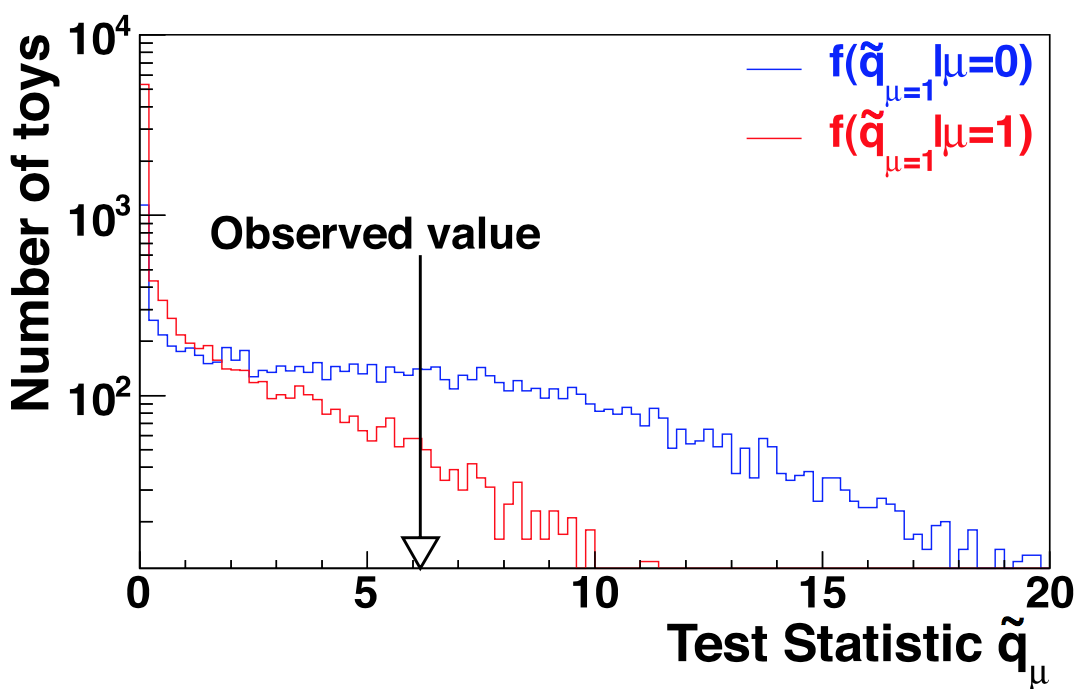
\includegraphics[width=0.70\textwidth]{plots_and_figures/chapter7/test_statistic_distri.png}
 \caption{Test statistic distributions for ensembles of pseudo-data generated for signal-plus-background (red) and background-only (blue) hypotheses.~\cite{note2011}}
 \label{fig:test_stat_dist}
\end{figure*}


Having constructed the above pdfs, it is now possible to calculate the probabilities of the observations under both hypotheses. The first quantity that we calculate is:
\begin{equation}                                                                                                                                                                                                 \label{eq:pmu}                                                       p_\mu=P(\tilde{q_\mu}\geq \tilde{q_\mu}^{obs}|\text{signal-plus-background})=\int_{\tilde{q_\mu}^{obs}}^{\inf}f(\tilde{q_\mu}|\mu,\hat{\theta_\mu}^{obs})d\tilde{q_\mu}
\end{equation}

The above quantity corresponds to CL$_\text{s+b}$ and measures the incompatibilty of data with signal-plus-background hypothesis. This quantity alone is not adequate for hypothesis testing in situations when the signal is so small that both hypotheses are compatible with the observation and a downward fluctuation of the background can lead to an inference of signal.

The second quantity we calculate is:
\begin{equation}                                                                                                                          
  \label{eq:pb}                                                     
  1-p_b=P(\tilde{q_\mu}\geq \tilde{q_\mu}^{obs}|\text{background-only})=\int_{\tilde{q_\mu}^{obs}}^{\inf}f(\tilde{q_\mu}|0,\hat{\theta_0}^{obs})d\tilde{q_\mu}                                                                                                            
\end{equation}
This quantity corresponds to CL$_\text{b}$ and measures the incompatibilty of data with the background. The incompatibilty of the data with background-only hypothesis alone doesn't tell us that it is indeed compatible with the signal, and so is not considered a good test of the signal hypothesis.

The ratio of the two quatities referred to as CL$_\text{s}$~\cite{cls1,cls2,cls3} helps deal with both situations above well, and is given by:
\begin{equation}                                                                                                                          
  \label{eq:cls}                                                                                                                           \text{CL}_\text{s}=\frac{p_\mu}{1-p_b}
\end{equation}

The 95\% CL is then arrived at by iterating over $\mu$ until we have CL$_\text{s}=0.05$. And the amount of signal or above, given by that $\mu$, denoted as $\mu^{95\%CL}$, is said to be excluded at 95\% CL. 

\subsection{Median expected Limits}

Upper exclusion limits calculated using toy datasets of background-only expectation, are called expected limits. A large set of background-only pseudo-data is generated, and CL$_\text{s}$ and $\mu^{95\%CL}$ is calculated for each of them. The median expected limit is calculated by integrating over this distribution until the 50\% quantile is reached. The $\pm 1\sigma$ bands are calculated similary by integrating the distribution to the appropiate quantiles are reached. The calculation of median expected limits does not involve using the observed data and hence can be calculated when the analyses is blinded to prevent experimenter's bias (as mentioned in Section~\ref{evt_sel_intro}). This can be use to maximize the sensitivity of the search, as described in Sections~\ref{h125_cb_sel} and ~\ref{H125_cb_sel}. A more stringent(lower) median limit corresponds to a more sensitive search.  


\subsection{Quantifying an excess of events}
\label{theo_uncert}
In case an excess of data over background is observed, it is necessary to make sure beyond a reasonable doubt that the excess is not merely a fluctuation. This is quantified using the background-only p-value, which is the probability for the background to fluctuate and give an excess of events as large or larger than that observed. The same test statistic as equation~\ref{eq:proflik} is used with the signal stength set to 0 to correspond to the background-only hypothesis:

\begin{equation}
\label{eq:proflik_b}
  \tilde{q_0}=-2\text{ ln}\frac{\mathcal{L}(\text{data}|0,\hat{\theta_0})}{\mathcal{L}(\text{data}|\hat{\mu},\hat{\theta})},\text{   with  } 0\leq\hat{\mu} 
\end{equation}
The constraint on $\hat\mu$ being greater than 0 is required so that a deficit of events in observed data is not interpreted in the same manner as we would an excess. In other words a departure from the background hypothesis in the form of deficit of events is not considered in favour of the signal hypothesis. Following the same procedure as calculation of observed limits ~\ref{exc_cal} and generating pseudo-data, the distribution $f(\tilde{q_0}|0,\hat{\theta_{0}}^{obs})$ is constructed. The p-value is then given by:

\begin{equation}                                                                                                                          
  \label{eq:p0}                                                     
  p_0=P(\tilde{q_0}\geq \tilde{q_0}^{obs})=\int_{\tilde{q_0}^{obs}}^{\inf}f(\tilde{q_0}|0,\hat{\theta_0}^{obs})d\tilde{q_0}               \end{equation}

The p-value can be converted to significance $\mathcal{Z}_0$, which is an equivalent way of quantifying an excess and is related to the p-value by the following:

\begin{equation}                                                                                                                          
  \label{eq:sig}                                                                                                                           p_0=\int_{\mathcal{Z}_0}^{\inf}\frac{1}{\sqrt{2\pi}}exp(-x^2/2)dx
\end{equation}

Broadly, the signficance corresponds to how far into the tail of the distribution (i.e., away from the most probable value), assuming background hypothesis, the test statistic value corresponding to the observed data lies. The farther it is, the less likely it is to have been a fluctuation. The conventional standard in high energy physics to be able to claim observation of a process is a significane of $5\sigma$, which corresponds to a p-value of $2.8\times 10^{-7}$.


\subsection{Systematic uncertainties}
\label{exp_uncert}
It is important to consider all relevant sources of uncertainties when perfoming sophisticated counting experiments such as these. Uncertainties that introduced as a result of imprecise/inaccurate knowledge of the system or gaps in prior knowledge that is used in the measurement are called systematic uncertainties. They are a different class of uncertainties than those arising purely out randomness in statistical measurements, called statistical uncertainties. The sources of systematic uncertainties range from purely theoretical in nature to purely experimental. They can be categorized in the two following ways:
\subsubsection{Normalization Uncertainties}
The value of these uncertainties are independent of the signal/discriminant variable. To be more precise, these uncertainties are independent of the value of $\mcol$ or BDT response. Hence, they effect each bin of those distributions in exactly the same manner and thus change only the overall scale of the distribution without altering its shape.

The muons in the analysis are required to pass certain identification, isolation and triggering criteria (see chapter~\ref{evt_sel}). The efficiencies for muon to pass these criteria are measured via tag-and-probe methods~\cite{muon_recon2018} using $Z\rightarrow\Pgm\Pgm$ events, and the scale factors are used to match the efficiency in MC to that in data. Briefly, the tag-and-probe method works in the following way. One of the muons (called the tag) is required to pass strict selection criterion, while the other (called the probe) is required to pass more relaxed criterion. Given the invariant mass of the $\Pgm-\Pgm$ system is required to within a very narrow  window of the Z mass, the probe muon is also very likely to be a real muon. The percentage of probe muons that pass the criterion we are testing for (identification, isolation, trigger etc.) gives the  efficiency. The efficiencies determined by this process, like any other quantity, are associated with systematic  uncertainties. For the muons used in the analyses described here, a combined normalization uncertainty of 2\% is associated with muon trigger, identification and isolation. Similar to muons, the efficiencies for electrons used in the analyses have also been measured via tag-and-probe methods~\cite{e_recon} using $Z\rightarrow\Pe\Pe$ events. The uncertainties in efficiencies  of electron identification and isolation criterion are also included as normalization uncertainty of 2\% in the fit. Both the above uncertainties are applied to processes which are derived from MC simulation. As mentioned earlier, a b tagging veto is applied to the analysis in order supress backgrounds involving top quarks. The efficiency of b tagging procedure is different in MC simulation than data. A scaling procedure is applied to match these efficiencies, and the uncertainties associated with these factors are found to not effect the shape of the $\mcol$ or BDT distributions. They are thus included in the fit as normalization uncertainties and range across categories from 2-4.5\% and 2-2.5\% for $\hmue$ and $\Hmue$ analysis respectively.

Several backgrounds in the analyses are estimated using MC simulations (see chapter ~\ref{bg_val}). These include \ztt,\ttb,\wjets, $\PW\PW$, $\PW\PZ$ and $\PZ\PZ$, $Z\to\ell\ell$ $(\ell = \Pe, \Pgm)+\text{jets}$, single-top quark production, $\PW\gamma^{(*)}+\text{jets}$. The production cross-sections for these backgrounds determine the number of events each background would contribute. These cross-sections are measured experimentally and the uncertainty in those measurements are included in the fit. Given that a change in cross-section changes the overall number of events produced, it has no effect on the shape of distributions. Hence these uncertainties are included as normalization uncertainties. These uncertainties in general  arise from: uncertainties on the parton distribution functions and strong coupling constant (called PDF+$\alpha_s$); variations in renormalization and factorization scales. In the $\Hmue$ analysis a applied separate uncertainty is applied for PDF+$\alpha_s$ and renormalization/factorization scales for each of the backgrounds. In $\hmue$ analysis, a combined uncertainty for each background is applied to cover both sources. All the above uncertainties are considered 100\% correlated among categories. For each background, an 5\% uncertainty, uncorrelated among all categories, is also applied to conservatively cover differences across categories. The QCD multijet background is estimated using a data-driven procedure. An uncertainty of 30\% associated with this (corresponding to the uncertainty in the extrapolation factor from the same-sign to opposite-sign region) is included in the fit. All uncertainties are summarized in table ~\ref{table:syst}.

\begin{table*}[htpb]
  \begin{center}
    \caption{The systematic uncertainties for the four channels. All uncertainties are treated as correlated between the categories, except those with more values separated by the $\oplus$~symbol. In the case of two values, the first value is the correlated uncertainty and the second value is the uncorrelated uncertainty for each individual category. In the case of three values, the first and second values correspond to the uncertainties arising from factorization and renormalization scales and PDF variations and are correlated between categories, while the third value is the uncorrelated uncertainty for each individual category. Two values separated by the "--" sign represent the range of the uncertainties from the different sources and/or in the different jet categories. %Anticorrelations arise due to  migration of events between the categories and are expressed as negative numbers.
    }
    [\cmsTabSkip]
%\scalebox{0.87}{
\begin{tabular}{l*{2}{c}} \hline
Systematic  uncertainty            & $\hmue$& $\Hmue$  \\ \hline
Muon  trigger/ID/isolation         &       2\%             &       2\%         \\
Electron trigger/ID/isolation      &       -             &       2\%           \\
b tagging veto                     &      2.0--2.5\%       &      2.0--2.5\%         \\ 
[\cmsTabSkip]
QCD multijet background            &      -              &       30\%                \\
$\ztt+\textrm{jets}$ background &     0.1\%$\oplus$2\%$\oplus$5\%   & 0.1\%$\oplus$2\%$\oplus$5\%         \\
$\ttb$ background                &     10\%$\oplus$5\%   &   10\%$\oplus$5\%              \\
$W+\textrm{jets}$ background     &     -               &                  \\
$\PW\PW,\PZ\PZ,\PW\PZ$ background&                  &\\
$\PW\gamma^{(*)}+\text{jets}$ background           &     -               &   10\%$\oplus$5\%            \\
Single top quark background        &     3\%$\oplus$5\%$\oplus$5\%    &   --              \\ 
$Z\to\ell\ell$ $(\ell = \Pe, \Pgm)+\text{jets}$ background&     -               & 0.1          \\
%BR(SM H$\rightarrow\tau\tau$) theory  &     0.62 -- 1.7 \%    &   0.62 -- 1.7 .7 \%    \\
[\cmsTabSkip]
Jet energy scale                   &        3--20\%        &        3--20\%                         \\
$\Pgm$ energy scale                &        0.2\%          &        0.2\%                              \\
$\Pe$ energy scale                 &        -            &         0.1--0.5\%                          \\
Unclustered energy scale           &        $\pm 1 \sigma$ &  $\pm 1 \sigma$                            \\
[\cmsTabSkip]
Integrated luminosity              &              2.5\%    &       2.5\%                                        \\ \hline
\end{tabular}%}
\label{table:syst}
\end{center}
\end{table*}


Just like MC backgrounds described above, the signal in both $\hmue$ and $\Hmue$ analysis comes from MC simulation. The signal process and the SM Higgs background are associated with uncertainties in the Higgs boson production cross sections. These come from variations in factorization/renormalization scales, as well as PDF+$\alpha_s$, and result in changes only in normalization. These uncertainties are summarized for SM Higgs boson and heavier Higgs of different masses in table~\ref{table:syst}. They are taken from Handbook of LHC Higgs cross-sections found in Ref.~\cite{YR4}.

\begin{table*}[!htbp]
  \begin{center}
  \caption{ Theoretical uncertainties from~\cite{YR4} are applied to the Higgs boson production cross sections for the different masses. In the reference, the PDF and $\alpha_s$ uncertainties are computed following the recommendation of the PDF4LHC working group. The remaining Gaussian uncertainty accounts for additional intrinsic sources of theory uncertainty described in detail in the reference.}
  \begin{tabular} {cccc}
    \hline
    $m_{\PH}$  (GeV) & Cross section (pb) &Theory, Gaussian (\%) & PDF$+\alpha_s$  (\%)\\\hline
200 & 16.94
&$\pm$1.8
&$\pm$3.0\\
300
&6.59
&$\pm$1.8
&$\pm$3.0\\
450
&2.30
&$\pm$2.0
&$\pm$3.1\\
600
&1
&$\pm$2.1
&$\pm$3.5\\
750
&0.50
&$\pm$2.1
&$\pm$4.0\\
900
& 0.27
&$\pm$2.2
&$\pm$4.6\\\hline
  \end{tabular}
  \label{tabe:syst_signal}
\end{center}
\end{table*}



The estimation of a particular background, that is derived from simulation, needs to correspond to the number of events (of that background, having a particular cross-section) that would be produced in the amount proton-proton collision data that we are using for this search. In other words, the background estimations need to be normalized to the integrated luminosity of the data collected. Integrated luminosity (defined in chapter~\ref{chap:exper_setup} is a measured quantity, and like all measured quantities, has an uncertainty associated with it. This amounts to 2.5\% and, like other normalization unceratainties, only effects only the overall scale of distributions.  







\subsection{Signal extraction}
\label{sig_ext}


\section{Heavy Higgs Analysis}
\label{hh_sys}

\subsection{Theoretical uncertainties}
\label{theo_uncert}

\subsection{Experminetal uncertainties}
\label{exp_uncert}

\subsection{Signal extraction}
\label{sig_ext}

% % uncomment the following lines,
% if using chapter-wise bibliography
%
% \bibliographystyle{ndnatbib}
% \bibliography{example}




%
%
% Chapter 8
%

\chapter{Results}
\epigraph{There are two possible outcomes: if the result confirms the hypothesis, then you've made a measurement. If the result is contrary to the hypothesis, then you've made a discovery.}{\textit{Enrico Fermi}}
\label{results}
\vskip 0.6in
In this chapter the results of both the searches are presented. The results for the $\hmue$ search are first presented. Results for the $\Hmue$ search follow.

\section{$\hmue$ results}
The resulting distributions of the signal variable (after applying all selection requirements as outlined in ~\ref{h125_evt_sel}) are fit using a binned maximum likelihood fit. The entire procedure is described in detail in ~\ref{stat_meth}. All systematic uncertainties are included as nuisance parameters, and the fit is performed simultaneously across all categories. The BDT response distributions of signal and background are shown superimposed for each category in Fig~\ref{fig:BDT_dist_hmue}. The distribution of $\mcol$ for the $\mcol$-fit analysis are also shown in Fig~\ref{fig:mcol_dist_hmue}. We do not observe an excess of signal over expected background. Hence, upper exclusion limits on $\mathcal{B}(\hmue)$ are set, following the procedure described in~\ref{exc_cal}. In table 8.1, the median expected limits, observed limits and the best fit branching fractions for $\mathcal{B}(\hmue)$ are summarized. As noted earlier in this thesis, the tau lepton coming from the Higgs can also decay hadronically. This channel of the LFV Higgs decay, i.e. $\hmuhad$ is studied in an analyses by different members of the same research team~\cite{HIG-17-001}. The limits on $\mathcal{B}(\hmuhad)$ from that search are combined with limits on $\mathcal{B}(\hmue)$, as calculated above from the search described here. All limits are summarized graphically in Figure~\ref{fig:hmue_limits_brazil}. The combined observed (median expected) upper limits on $\mathcal{B}(\hmu)$ is 0.25 (0.25)\,\% at 95\% CL, for the BDT-fit analysis. The combined best fit branching fraction of $\mathcal{B}(\hmu)$ is found to be $0.00 \pm 0.12$, also for the BDT-fit analysis. Figure~\ref{fig:hist_limits} shows a historical compilation of results from $\hmue$ searches until 2017. It is important to note that the 2.4\,$\sigma$ excess observed by the earlier CMS search with 8 TeV data~\cite{Khachatryan:2015kon} has now been excluded by this search.


\begin{table}[!htpb]
 \begin{center}
   \caption{Expected and observed upper limits at 95\% CL, and best fit branching fractions in percent for each individual jet category, and combined, for the $\hmue$ analysis}
   \scalebox{0.85}{
\begin{tabular}{*{6}{c}}
\multicolumn{6}{c}{Expected limits~(\%) } \\ \hline
                       &  \multicolumn{1}{c}{0-jet}   & \multicolumn{1}{c}{1-jet}    &  \multicolumn{1}{c}{2-jets ggH} & \multicolumn{1}{c}{2-jets VBF}  & \multicolumn{1}{c}{Combined}                 \\  \cline{2-6}
BDT fit analysis 	 &  $<$0.83   	 &  $<$1.19   	 &  $<$1.98   	 &  $<$1.62   	 &  $<$0.59    \\
$\mcol$ fit analysis 	 &  $<$1.01   	 &  $<$1.47   	 &  $<$3.23   	 &  $<$1.73   	 &  $<$0.75    \\
\cline{2-6}
\\ [\cmsTabSkip]
\multicolumn{6}{c}{Observed limits~(\%)} \\ \hline
                       &  \multicolumn{1}{c}{0-jet}   & \multicolumn{1}{c}{1-jet}    &  \multicolumn{1}{c}{2-jets} & \multicolumn{1}{c}{VBF} &\multicolumn{1}{c}{Combined}                 \\ \cline{2-6}
BDT fit analysis   		 & $<$1.30   	 & $<$1.34   	 & $<$2.27   	 & $<$1.79   	 & $<$0.86    \\
$\mcol$ fit analysis   		 & $<$1.08   	 & $<$1.35   	 & $<$3.33   	 & $<$1.40   	 & $<$0.71    \\
\cline{2-6}
\\[\cmsTabSkip]
\multicolumn{6}{c}{Best fit branching fractions~(\%)} \\ \hline
                       &  \multicolumn{1}{c}{0-jet}   & \multicolumn{1}{c}{1-jet}    &  \multicolumn{1}{c}{2-jets} & \multicolumn{1}{c}{VBF} &\multicolumn{1}{c}{Combined}                 \\  \cline{2-6}
BDT fit analysis    		 & 0.61 $\pm$ 0.36  	 & 0.22 $\pm$ 0.46  	 & 0.39 $\pm$ 0.83  	 & 0.10 $\pm$ 1.37  	 & 0.35 $\pm$ 0.26  \\
$\mcol$ fit analysis    		 & 0.13 $\pm$ 0.43  	 & $-0.22$ $\pm$ 0.75  	 & 0.22 $\pm$ 1.39  	 & $-1.73$ $\pm$ 1.05  	 & $-0.04$ $\pm$ 0.33  \\
\cline{2-6}
combined $\Pgm\Pgt$ (BDT fit)  & \multicolumn{5}{c}{ 0.00 $\pm$ 0.12 } \\ \hline
\end{tabular}}
\end{center}
\label{table:hmue_limits}
\end{table}

\begin{figure*}[!htpb]\centering
   \captionsetup{width=.98\textwidth,justification=centering}
 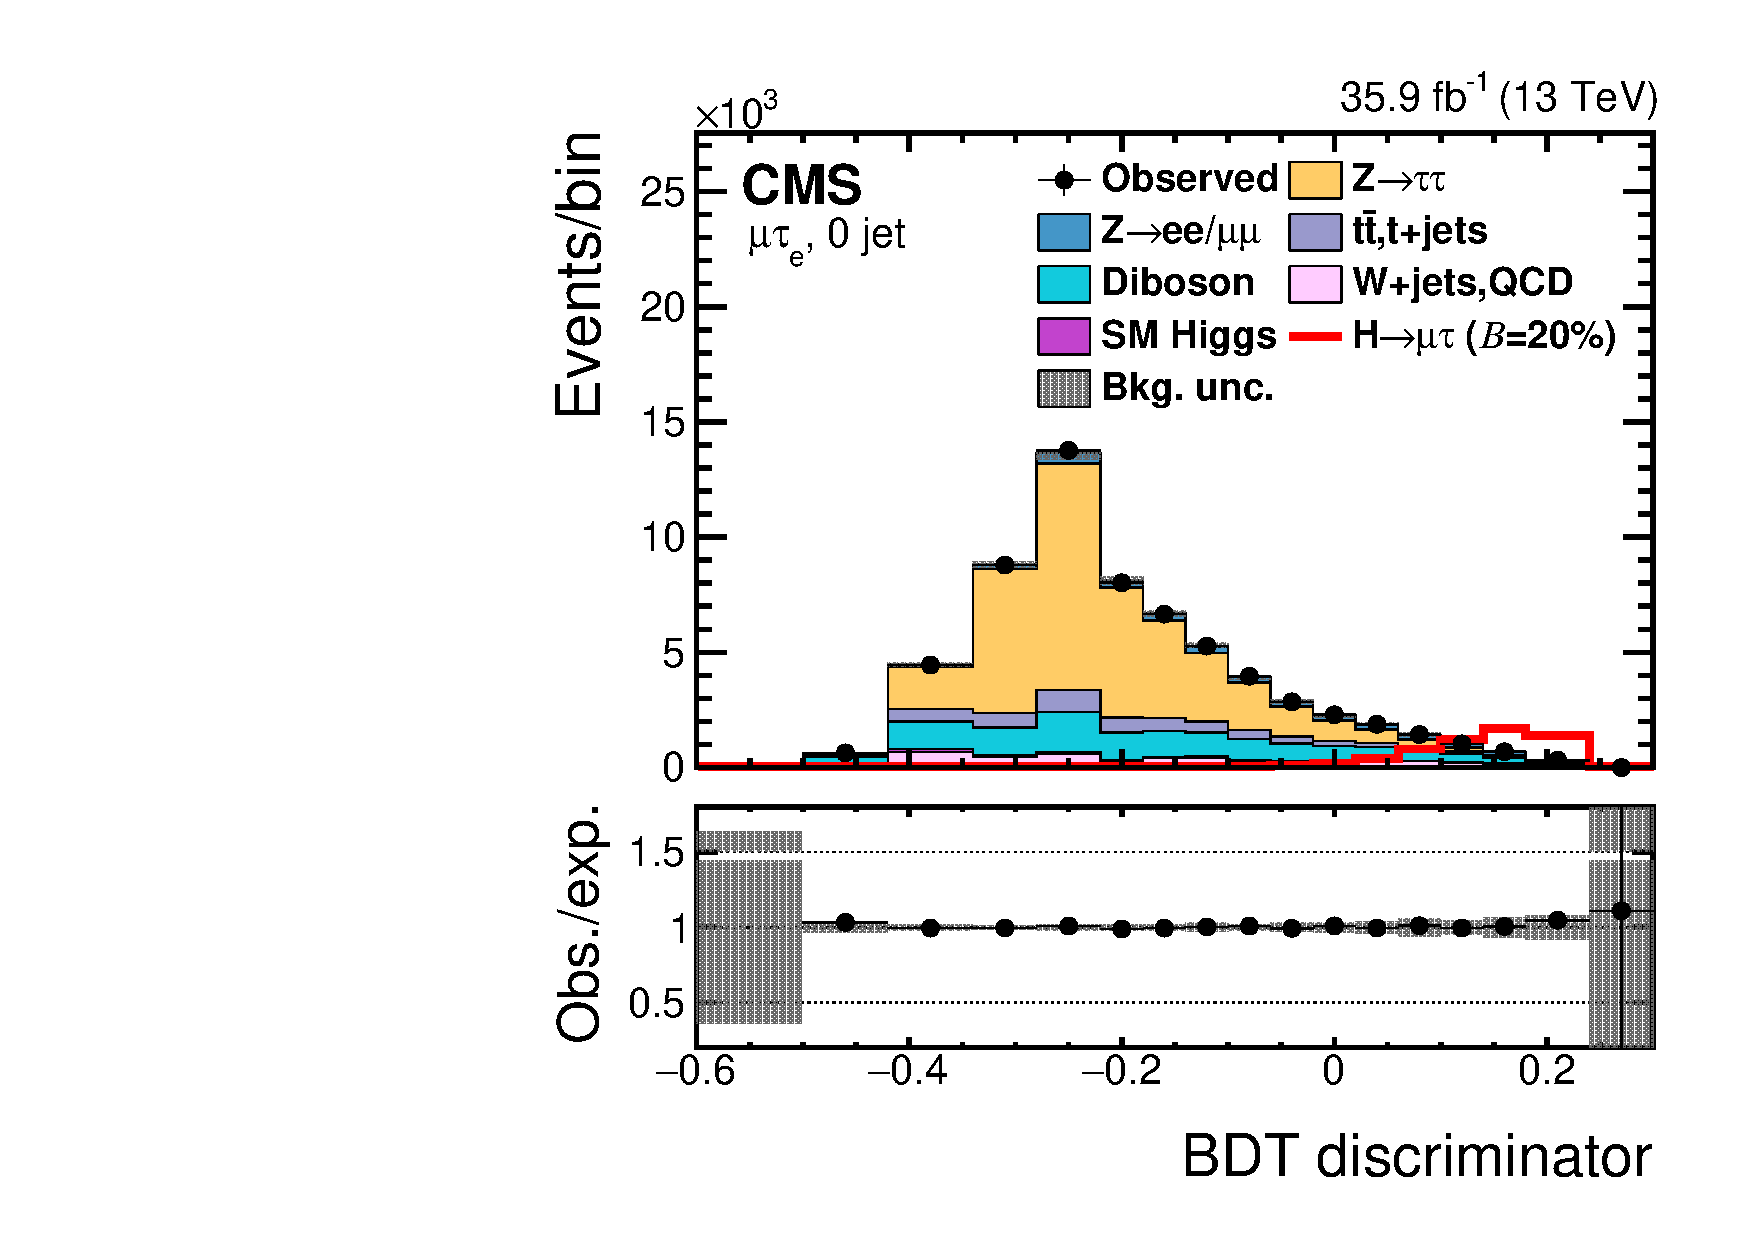
\includegraphics[width=0.49\textwidth]{plots_and_figures/chapter8/h125/0jetBDT.pdf}
 \includegraphics[width=0.49\textwidth]{plots_and_figures/chapter8/h125/1jetBDT.pdf} \\
 \includegraphics[width=0.49\textwidth]{plots_and_figures/chapter8/h125/2jetggBDT.pdf}
 \includegraphics[width=0.49\textwidth]{plots_and_figures/chapter8/h125/2jetvbBDT.pdf} 
\caption{Distribution of BDT response in each category comparing signal and background estimations to observed collision data, for $\hmue$ analysis. The bottom panel show the ratio of observed data and fitted background in each bin~\cite{HIG-17-001}.}
 \label{fig:BDT_dist_hmue}
\end{figure*}

\begin{figure*}[!htpb]\centering
   \captionsetup{width=.98\textwidth,justification=centering}
 \includegraphics[width=0.49\textwidth]{plots_and_figures/chapter8/h125/0jetmcol.pdf}
 \includegraphics[width=0.49\textwidth]{plots_and_figures/chapter8/h125/1jetmcol.pdf} \\
 \includegraphics[width=0.49\textwidth]{plots_and_figures/chapter8/h125/2jetggmcol.pdf}
 \includegraphics[width=0.49\textwidth]{plots_and_figures/chapter8/h125/2jetvbmcol.pdf} 
\caption{Distribution of $\mcol$ response in each category comparing signal and background estimations to observed collision data, for $\hmue$ analysis. The bottom panel show the ratio of observed data and fitted background in each bin~\cite{HIG-17-001}.}
 \label{fig:mcol_dist_hmue}
\end{figure*}

\begin{figure*}[!htpb]\centering
   \captionsetup{width=.96\textwidth,justification=centering}
 \includegraphics[width=0.49\textwidth]{plots_and_figures/chapter8/h125/brazilflagBDT.pdf}
 \includegraphics[width=0.49\textwidth]{plots_and_figures/chapter8/h125/brazilflagmcol.pdf} \\
 \caption{Observed and median expected upper exclusion limits for $\hmue$, $\hmuhad$ and combined $\hmu$ channels, for the BDT fit (left) and $\mcol$ fit analysis (right). The $\pm 1 \sigma$ and $\pm 2 \sigma$ bands for expected limits are also shown in light green and yellow respectively~\cite{HIG-17-001}.}
 \label{fig:hmue_limits_brazil}
\end{figure*}

\begin{figure*}[!htpb]\centering
 \captionsetup{width=.8\textwidth,justification=centering}
 \includegraphics[width=0.8\textwidth]{plots_and_figures/chapter8/h125/hist_limit.png}
 \caption{Historical compilation of results from direct searches for $\hmu$ decay. This search is represented by the rightmost point.}
 \label{fig:hist_limits}
\end{figure*}


The constraints on $\mathcal{B}(\hmu)$ can be transformed into constraints on Lepton Flavor Violating Yukawa Couplings ($Y_{\Pgm\Pgt},Y_{\Pgt\Pgm}$). These couplings represent the strength of an interaction and are related to the decay width $\Gamma(\hmu)$ in the following way~\cite{Harnik:2012pb}:
\begin{equation}                                                                                                                                                                                                 
\Gamma(\hmu)=\frac{m_{h}}{8\pi}(|Y_{\Pgm\Pgt}|^2 + |Y_{\Pgt\Pgm}|^2).                                                          
\label{eq:yuk1}
\end{equation}

The decay width is also related to the branching fraction, $\mathcal{B}(\hmu)$ according to the following equation:
\begin{equation}                                                                                                                                                                                                \mathcal{B}(\hmu)=\frac{\Gamma(\hmu)}{\Gamma(\hmu) + \Gamma_{SM}}.
\label{eq:yuk2}
\end{equation}
where the SM Higgs decay width is assumed to be $\Gamma_{SM}=4.1$ MeV~\cite{Denner:2011mq} for $m_{\PH}=125$\GeV. Using equations~\ref{eq:yuk1} and ~\ref{eq:yuk2}, we derive the constraints on Yukawa couplings at 95\% CL. The limits for the Yukawa couplings are summarized in Table~\ref{table:yuk_coup}. Fig.~\ref{fig:yuk_coup} pictorially summarizes all existing limits on Yukawa couplings from different direct and indirect searches. It also shows the theoretical ``naturalness'' limit considering/expecting LFV couplings to be smaller than those of couplings for SM decays of the Higgs~\cite{Harnik:2012pb}, which can be considered a benchmark for sensitivity of this search. The limits derived from this search are most stringent till date, and surpass the above benchmark. 

\begin{table}[!hbtp]
 \centering
  \caption{95\% CL observed upper limit on the Yukawa couplings, for the BDT fit and the \mcol fit analysis}
 \label{table:yuk_coup}
\begin{tabular}{|ccc| }
   \hline
                        & BDT fit  &  \mcol fit \\ \hline
$\sqrt{|Y_{\Pgm\Pgt}|^{2}+|Y_{\Pgt\Pgm}|^{2}}$   & $<1.43\times 10^{-3}$ &  $<2.05\times 10^{-3}$  \\
  \hline
\end{tabular}
\end{table}

\begin{figure*}[!htpb]
  \centering
   \captionsetup{width=.9\textwidth,justification=centering}
 \includegraphics[width=0.9\textwidth]{plots_and_figures/chapter8/h125/yukawa.pdf}
 \caption{Observed (black solid)and median expected (red dashed) upper limits on $\hmu$ Yukawa couplings from this analysis. The light green and yellow bands show the $\pm 1 \sigma$ and $\pm 2 \sigma$ spreads of the expected limit. Blue solid line shows the result from the previous CMS search with 8 TeV data~\cite{Khachatryan:2015kon}. The naturalness limit is shown as a purple straight line~\cite{HIG-17-001}.}
 \label{fig:yuk_coup}
\end{figure*}


\section{$\Hmue$ results}
The resulting $\mcol$ distributions for signal and background estimation (after applying all selection requirements as outlined in ~\ref{HH_evt_sel}), after a binned maximum likelihood fit, are shown superimposed along with the observed data Fig~\ref{fig:mcol_dist_Hmue}. All systematic uncertainties are included as nuisance parameters, and the fit is performed simultaneously across all categories. We do not observe an excess over expected background in the entire range. Unlike the $\hmue$ analysis described above where the production cross-section of the SM Higgs boson is known, here we are looking for LFV decay of a hypothetical heavy Higgs bosons of different masses. Hence, we set upper exclusion limits on production cross-section times branching fraction, $\sigma(\textrm{gg}\rightarrow \PH)\times\mathcal{B}(\Hmue)$. The procedure is the same as used above and described in~\ref{exc_cal}. The observed and median expected upper limits at 95\% CL on $\sigma(\textrm{gg}\rightarrow \PH)\times\mathcal{B}(\Hmue)$ are summarized in table~\ref{table:limits_Hmue} for different categories and Higgs masses. The limits are also summarized graphically in Figure~\ref{fig:limits_Hmue}. The observed (median expected) limits range from 159.4 (95.6)\,pb to 2.9 (4.9)\,pb for heavy Higgs masses in the range between 200 and 900\,GeV. This search was combined with LFV heavy Higgs decay search with the tau lepton decaying hadronically, i.e. $\Hmuhad$ to produce constraints $\Hmu$. The combined observed (median expected) upper limits on $\sigma(\textrm{gg}\rightarrow \PH)\times\mathcal{B}(\Hmu)$ range from 51.9 (57.4)\,pb to 1.6 (2.1)\,pb. These limits are shown graphically in Figure~\ref{fig:limits_Hmu}. This is the first direct search till date to set limits on this decay.      

\begin{figure*}[!htpb]\centering
   \captionsetup{width=.98\textwidth,justification=centering}
 \includegraphics[width=0.49\textwidth]{plots_and_figures/chapter8/highmass/log_low_me_ch1_HMuTau_mutaue_1_2016_postfit_colmass_postfit.pdf}
 \includegraphics[width=0.49\textwidth]{plots_and_figures/chapter8/highmass/log_low_me_ch1_HMuTau_mutaue_2_2016_postfit_colmass_postfit.pdf} \\
 \includegraphics[width=0.49\textwidth]{plots_and_figures/chapter8/highmass/log_high_me_ch1_HMuTau_mutaue_1_2016_postfit_colmass_postfit.pdf}
 \includegraphics[width=0.49\textwidth]{plots_and_figures/chapter8/highmass/log_high_me_ch1_HMuTau_mutaue_2_2016_postfit_colmass_postfit.pdf} 
\caption{Distribution of $\mcol$ in 0-jet (left) and 1-jet (right) for lowmass (top) and highmass (range), comparing signal and background estimations to observed collision data, for $\Hmue$ analysis. The bottom panel show the ratio of observed data and fitted background in each bin~\cite{HIG-18-017}.}
 \label{fig:mcol_dist_Hmue}
\end{figure*}


\begin{figure*}[!htpb]\centering
   \captionsetup{width=.98\textwidth,justification=centering}
 \includegraphics[width=0.49\textwidth]{plots_and_figures/chapter8/highmass/Figure_004-c.pdf}
 \includegraphics[width=0.49\textwidth]{plots_and_figures/chapter8/highmass/Figure_004-d.pdf} \\
 \includegraphics[width=0.60\textwidth]{plots_and_figures/chapter8/highmass/Figure_005-b.pdf}
\caption{Observed and Median expected 95\% upper exclusion limits for 0-jet (upper left), 1-jet (upper right) and combined (bottom),for the $\Hmue$ analysis~\cite{HIG-18-017}.}
 \label{fig:limits_Hmue}
\end{figure*}



\begin{table}
\caption{The observed (median expected) 95\% CL upper limits on $\sigma(\textrm{gg}\rightarrow \PH) \times\mathcal{B}(\Hmue)$}
\begin{center}
\begin{tabular}{c|c|c|c}
\hline
$m_{\PH}$ (GeV) & 0 jet & 1 jet  & comb\\
\hline
200 &147.8 (107.5) & 262.1 (209.8)& 159.4 (95.6) \\
300 &30.1 (49.8) & 100.8 (108.6) & 29.3 (45.2) \\
450 &31.1 (17.5) & 35.3 (32.8) )& 23.7 (20.4) \\
600 &8.1 (10.4)& 15.2 (17.9)& 6.8 (8.9) \\
750 &6.5 (8.0)& 7.8 (18.2)& 4.7 (6.1) \\
900 &4.4 (6.9)& 5.6 (15.4)& 2.9 (4.9) \\
\hline
\end{tabular}
\label{table:limits_Hmue}
\end{center}
\end{table}


\begin{figure*}[!htpb]
  \centering
   \captionsetup{width=.8\textwidth,justification=centering}
 \includegraphics[width=0.8\textwidth]{plots_and_figures/chapter8/highmass/Figure_005-c.pdf}
\caption{Observed and Median expected 95\% upper exclusion limits for combined $\Hmu$ analysis~\cite{HIG-18-017}.}
 \label{fig:limits_Hmu}
\end{figure*}



% % uncomment the following lines,
% if using chapter-wise bibliography
%
% \bibliographystyle{ndnatbib}
% \bibliography{example}


%
%
% Chapter 7
%

\chapter{Conclusion}
\label{conclusion}

% % uncomment the following lines,
% if using chapter-wise bibliography
%
% \bibliographystyle{ndnatbib}
% \bibliography{example}

%
% Appendix (optional)
%

%\appendix

%\chapter{Boosted Decision Trees}
\label{chap_BDT} 

\section{Introduction}
%\include{appendixB}

%
% Back stuff
%

% % comment out the following three lines
% if using chapter-wise bibliography

 \backmatter

  \bibliographystyle{unsrtnat}%\bibliographystyle{abbrvnat} % The standard abbrvnat style should be acceptable. Also provided with both the advanced and standard
  \bibliography{thesis_v0}  % distributions are nddiss2e and nddiss2enoarticletitles style options.
% If you prefer to manually enter your bibliography, that is fine. Comment out the previous two lines, and enter your bibliography
% as usual. Note that if you choose this route, formatting the bibliography is your responsibility. An example is below, including the
% optional arguments necessary for author-date style citations.
%	\begin{thebibliography}{9}
%		\bibitem[Galmira(1998)]{galmira98:_gnus_milit} G.\ Galmira. Gnus and the military -- a secret conspiracy? \emph{Growing Towards Gnu}, III(7):22--183, September 1998.
%		
%		\bibitem[Ganston and Greenfield(1998)]{gnus98:_gerry_ganst} G.\ Ganston and G.\ Greenfield. \emph{Gnus and You: The Art of Being New}. volume I. Grapping Books, NY, August, 1998.
%		
%		\bibitem[Gloonston(1998)]{gloonston98:_gnuly_discov_gnus} G.\ Gloonston. Newly discovered gnus: The LoG. \emph{Growing Towards Gnu}, II(12):23---57, March 1998.
%		
%		\bibitem[Greenfield(1996)]{greenfield96:_gettin_know_gnu} G.\ Greenfield. \emph{Getting to Know Gnu}. PhD thesis, Geoffrey Garfield School of Gnus, August 1996.
%		
%		\bibitem[van Gairley(2000)]{gairley2000} G.\ van Gairley. Gnu's review. Website, 2000. \url{http://www.gairley.gnu}.
%	\end{thebibliography}

\end{document}

% End of ``example.tex''
